% !TEX root = thesis.tex

\chapter{Nonverbal Social Signal Prediction}
\label{chapter:prediction}
%
%%%%%%%%%% ABSTRACT
%\begin{abstract}
%   In this paper, we present a new research task to understand human social interactions via computational methods, to ultimately endow machines with the ability of encoding and decoding the social signals humans use. This research direction is essential to make machine that genuinely communicate with humans. We first formulate the social signal prediction problem as a way to model social behaviors by finding the implicit correlations among social signals in a data-driven way. We then present a new dataset, where the full-spectrum of multi-modal social signals (including face, body, and finger motions) are captured in a triadic social interaction scenario. Several baseline approaches and their results are presented to model social interactions in the presented social prediction framework. Finally we discuss the potential of this new task and guide the future directions. 
%\end{abstract}

%%%%%%%%% BODY TEXT

%\section{Introduction}
%The way humans communicate is one of the clearest factors that differentiates us from other animals. Along with verbal language, we use many other channels for communication, including eye contact, facial expression, body gestures, and hand motions, collectively referred to as non-verbal social signals~\cite{Moore13}. Notably, the use of all these channels is important in social interactions, where subtle emotions and intentions are transmitted via the combination of such signals. Endowing machines with such social interaction abilities is an essential goal of Artificial Intelligence (AI) to make machines that can effectively cooperate with humans. This area is related to multidisciplinary research fields covering psychology, natural language processing, affective computing, human-robot interaction, machine learning, and computer vision.


%A way to endow machines with such social skills would be to encode all the rules that humans observe during social communication. Unfortunately, nonverbal interaction is still poorly understood despite its importance in social communication~\cite{Mehrabian67,Mehrabian81,Birdwhistell-1970}, making it hard to formalize rules about how to understand and use social signals. Interestingly, we have recently witnessed a great achievement in Natural Language Processing showing the potential to make machines ``freely" communicate with humans using written language and speech~\cite{young2018recent}. This success has been lead by data-driven approaches leveraging large-scale language datasets and a powerful modeling tool, deep neural networks, to automatically learn the patterns of human verbal communication. Remarkably, these achievements have not made extensive use of the prior knowledge about grammar and the structure of languages that linguists have accumulated over centuries. Motivated by this, we may hypothesize that a similar approach can be applicable in modeling nonverbal communication. 


%However, there exists a fundamental difficulty in building a data-driven nonverbal communication model: the data is extremely rare. In the verbal language domain, words contain the full expressive power to record verbal signals by composition of a handful of discrete symbols. Especially on the Internet, there already exist millions of articles or dialogues which are readily usable for data-driven methods (either supervised or unsupervised). Similarly, speech audio can be readily digitized and large datasets are available. However, for non-verbal signals, how to ``record" or collect these signals is uncertain. Imagine a situation where a group of people are communicating in our daily life. The positions and orientations of individuals, their body gestures, gaze, and facial expressions (among others) are the data we are interested in. Notably, these ``social signals" emitted from all people in the group need to be collected simultaneously to study their correlation and causality. Although there also exist millions of videos where our daily activities---including social interactions---are captured on the Internet, these raw videos cannot be directly used to understand the rules of non-verbal interactions because we have to extract all semantic visual cues (relative location, face, body pose, and so on) from the raw pixels. %Fortunately, measuring human behavior including person detection~\cite{}, body pose estimation~\cite{}, face keypoint detection, hand keypoint estimation, markerless motion captures have all been greatly advanced, enabling us to collect non-verbal signal dataset.


% % Unfortunately, we haven't make the similar success in nonverbal language part, and the major difficulty hindering the progress is the lack of available dataset where computational methods can be tested. 

% Consider a situation where a group of people are communicating in our daily life. They first meet each other, and then they make a special formation to start the communication (either standing or sitting). Someone starts speaking while others may listen, and the speaking turns are circling here and there. Both speaker and listeners use additional channels to transmit additional information which is not fully conveyed by language only, such as hand gestures, facial expression, nodding, eye gaze direction and so on. All these signals and rules presented during the communication is the signals we want to model. But, how can we ``record" or measure these signals so that we can apply the computational methods? In verbal language, words have the full expressive power to record the signals. Especially in the Internet, there already exist tons of literature or dialogues specifying the language signals humans use in our daily life. There is no such complete data for the non-verbal signals. Although there exist millions of video data where our daily activities including social interaction in the Internet, these raw videos cannot be directly used to understand the rules of non-verbal interactions, because we have to extract all semantic visual cues (person location, face, body pose, and so on) out of the raw pixels, which is basically the goal of computer vision area. Notably, these signals should be handled for the visual footage where multiple people are naturally interacting. Due to the person's body orientation and occlusion issues, measuring such signals itself is a challenging problem, despite the great advances of the human detection, pose estimation, reconstruction area in computer vision.

Consider how humans are communicating. To convey our thought, emotions, and intentions, we use our voice, and face, and body by which we encode the internal messages. The social signals emiited by the display port is then sensed by another person, and interpreted as a messeage. Althought several approaches try to model the internal status~\cite{}, still how to represent the internal status is poorly understood.  

Interestingly, these social signals are extremely correlated each other~\cite{}. First the signals from an idividuals are correlations. The body and hands motion of the same person is extremely organized to express the internal status as a whole. And the signals among individuals are correlated. When we communicate, we anticipate the reaction of the communication partner, and not be surpirsed by them. For example, when we speak, we expect eye contact and nodding response. We expect the communication partner does not suddenly perform weird gestures and or unexpected behaviors. This is also closely related to the screening and diagossing autism spectrum disorder~\cite{stone2000brief, mathys2013beyond}. For example, during the test, the examiner monitor the behavior of the subject in an interactive, play-based tests,  assessing  social-communicative behaviors of the subject. These test are based on the assumption that there exist socially expected behaviors among communication for healthy subjects, and measure how the behavior of the subject is different from the expected healthy feedback.  

Therefore, we aim to model the correlation among signals in a datadriven way, rather than modeling the internal status of human's mind. Given the data of input and output, this is a supervised learning provded. The biggest challenge here is which data can be used and how to represent the signals to formulate this problem. Importantly, how to evaluate the output is also a crucial part of this direction.

In this chapter, we introduce a new research task with the long-term aim to build machines that can genuinely interact with humans using non-verbal signals. The key idea of this problem is to define the social interaction as a signal prediction problem among individuals involved. We formulate that humans are communicating by receiving a set of social signals from others and emitting response signals as output, which are again directed to others as inputs (illustrated in Fig.~\ref{fig:ssp_intro}). Thus, we hypothesize that the social behavior ability can be learned by finding the patterns between these signal flows. Importantly, we aim to include as many signal modalities as possible to study the correlation among social signals. Since studying this in-the-wild is hard due to limits of signal measurement technology (e.g., motion capture) as well as the large variety of interaction contexts, we collect a large-scale dataset where these signals are accurately measured for naturally interacting people in a specific triadic social interaction scenario. Our dataset includes about 180 sequences of the negotiation game protocol, where 120 subject participated. We use the state-of-the art markerless motion capture technology~\cite{joo2018} to measure various social signal indicators. We use a deep neural network to model the social signal prediction problem. We study various types of human behaviors including proxemics, F-formation, and body gestures, and speaking timing. In this paper, we introduce several baseline results for the social signal prediction task. 

%In summary, we present:
%\begin{itemize}
%    \item A new dataset of triadic interactions with full spectrum capture of social signals. 
%    \item A formal definition of the problem for social signal prediction
%    \item Several baseline initial outputs in several scenarios
%\end{itemize}
%
%\begin{figure}
%	\centering
%	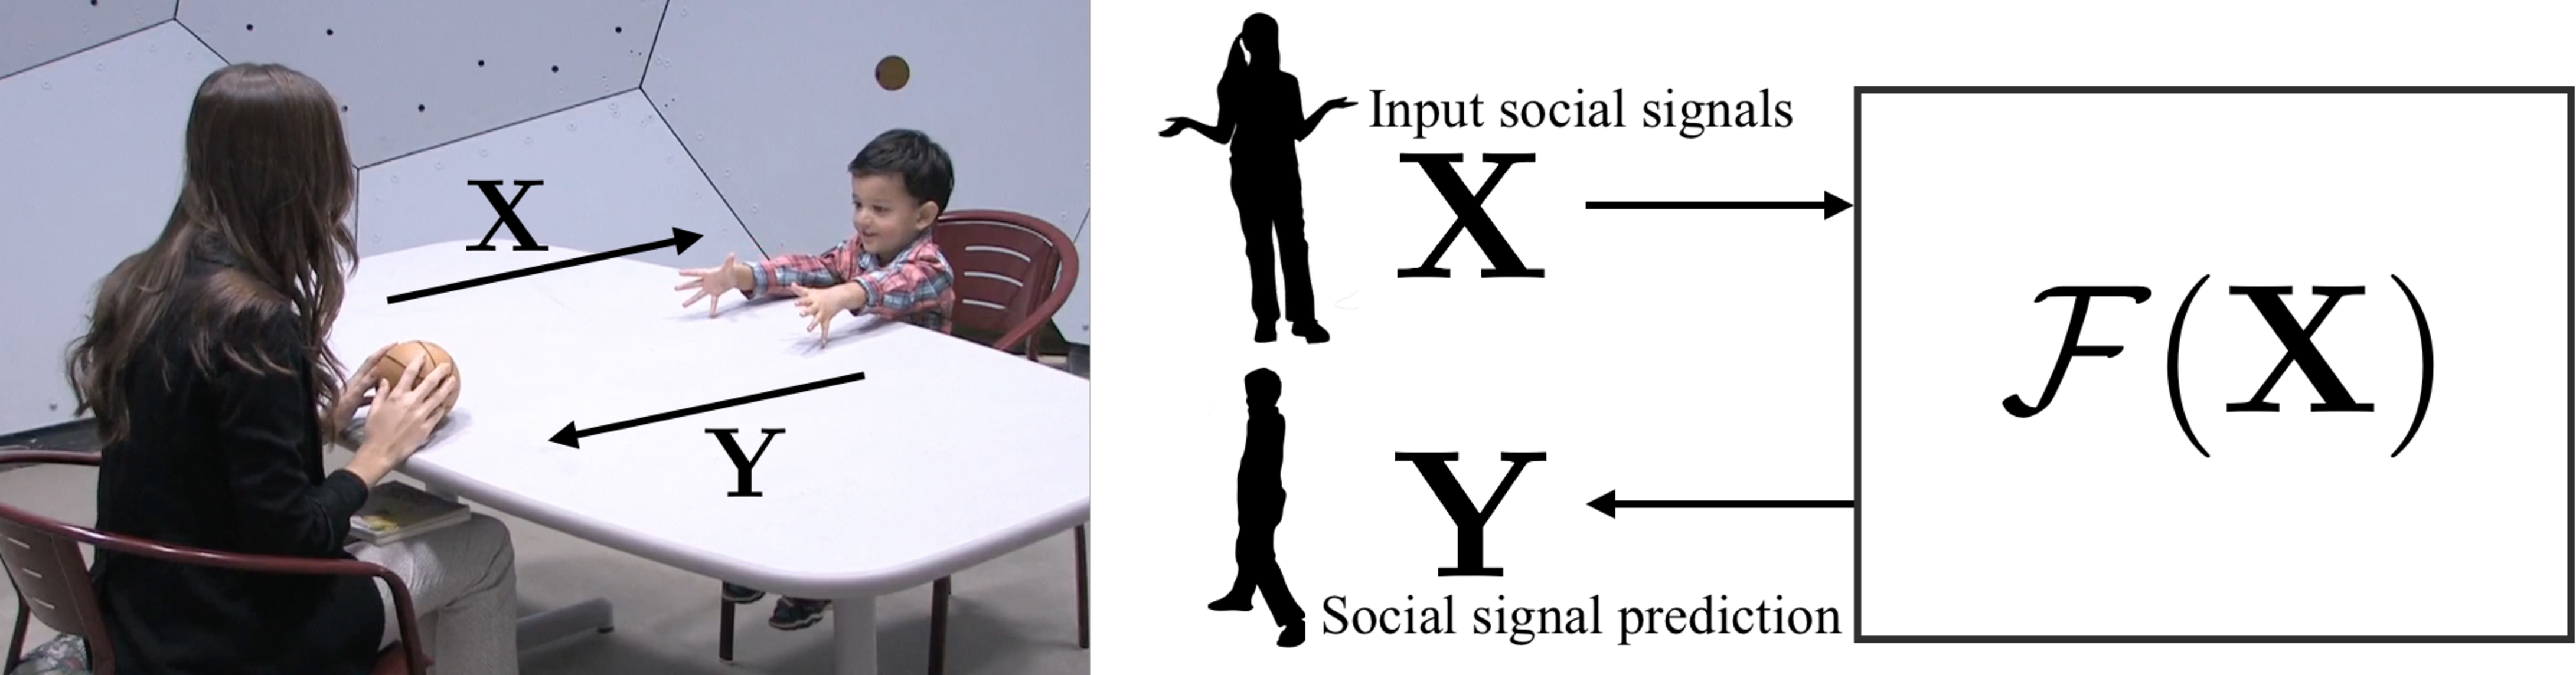
\includegraphics[width=\linewidth]{ssp_fig/intro}
%	\caption{We aim to build social artificial intelligence by building a model to learn the correlation between the input and output social signals. (Left) An example scene of RAPID-ABC test to detect autism spectrum disorder ~\cite{mathys2013beyond} and (Right) An illustration to describe social signal prediction task.}
%	\label{fig:ssp_intro}
%\end{figure}
\begin{figure}[t]
	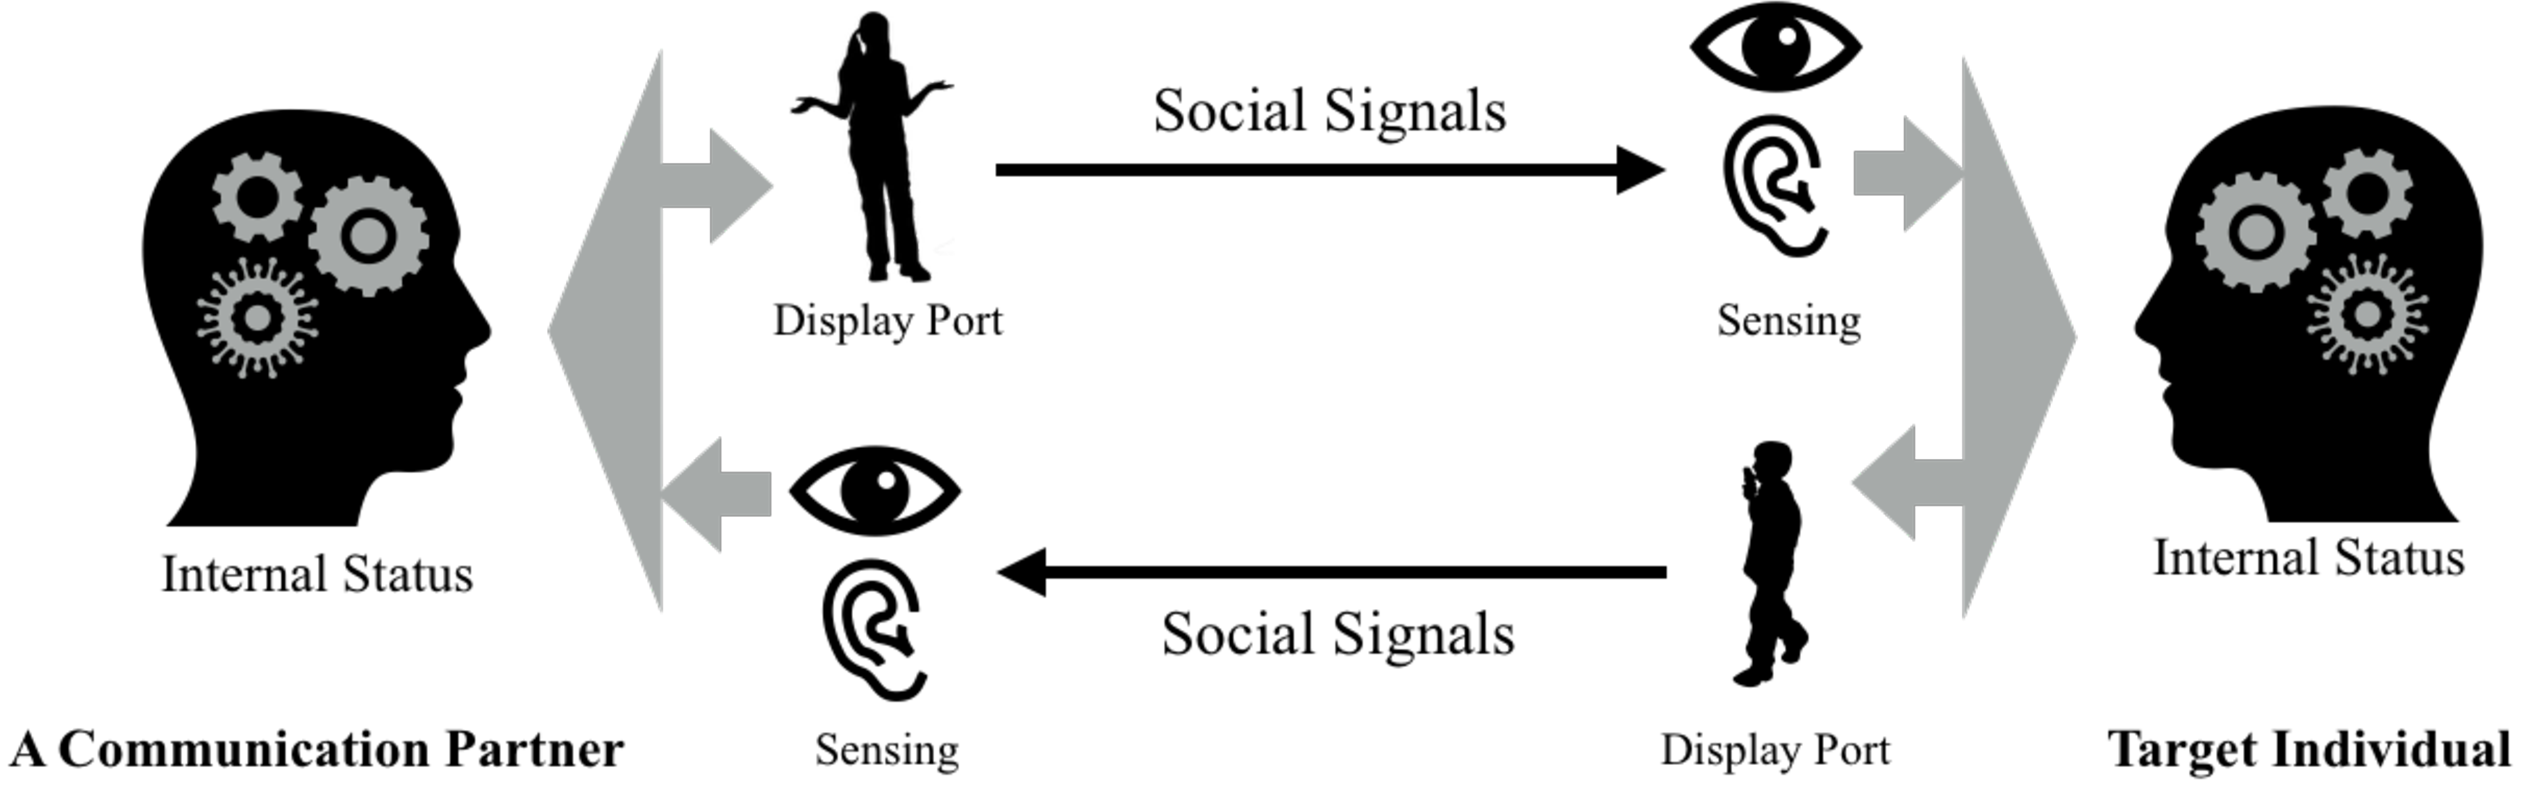
\includegraphics[width=\linewidth]{ssp_fig/socialcomm}
	\caption{Social Communication Flow}
\label{fig:ssp_intro_flow}
\end{figure}
\begin{figure}[t]
	\centering
	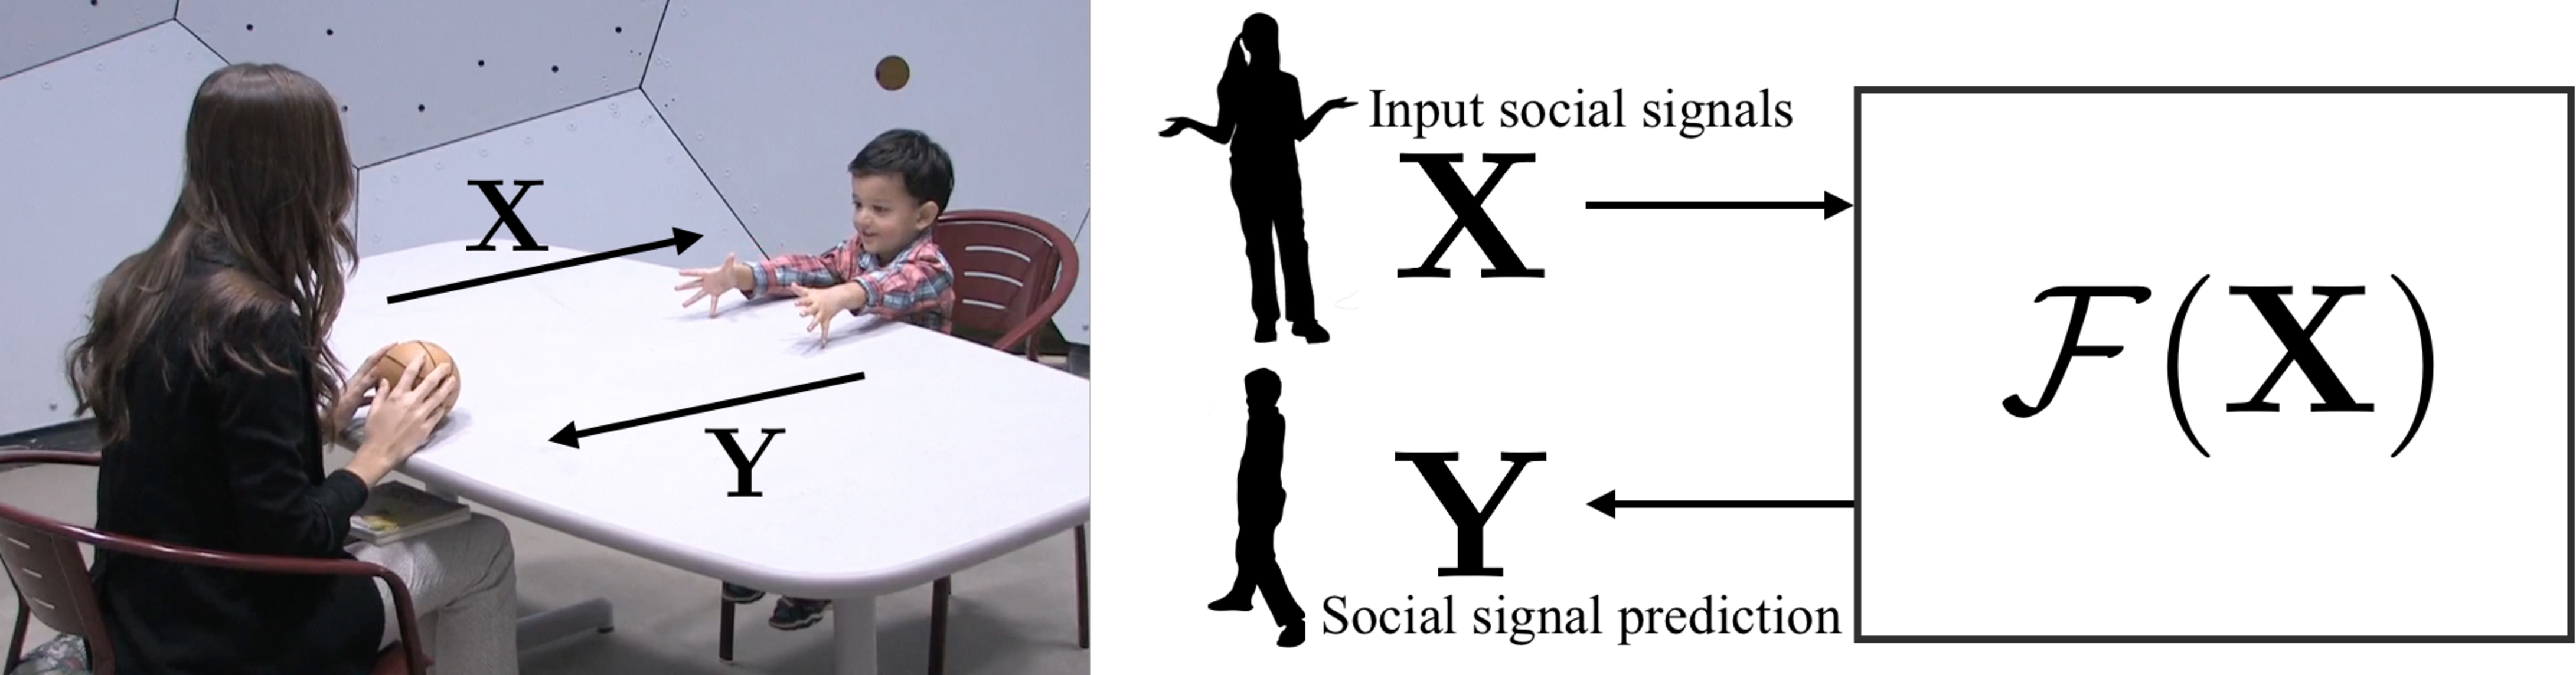
\includegraphics[width=\linewidth]{ssp_fig/intro}
%	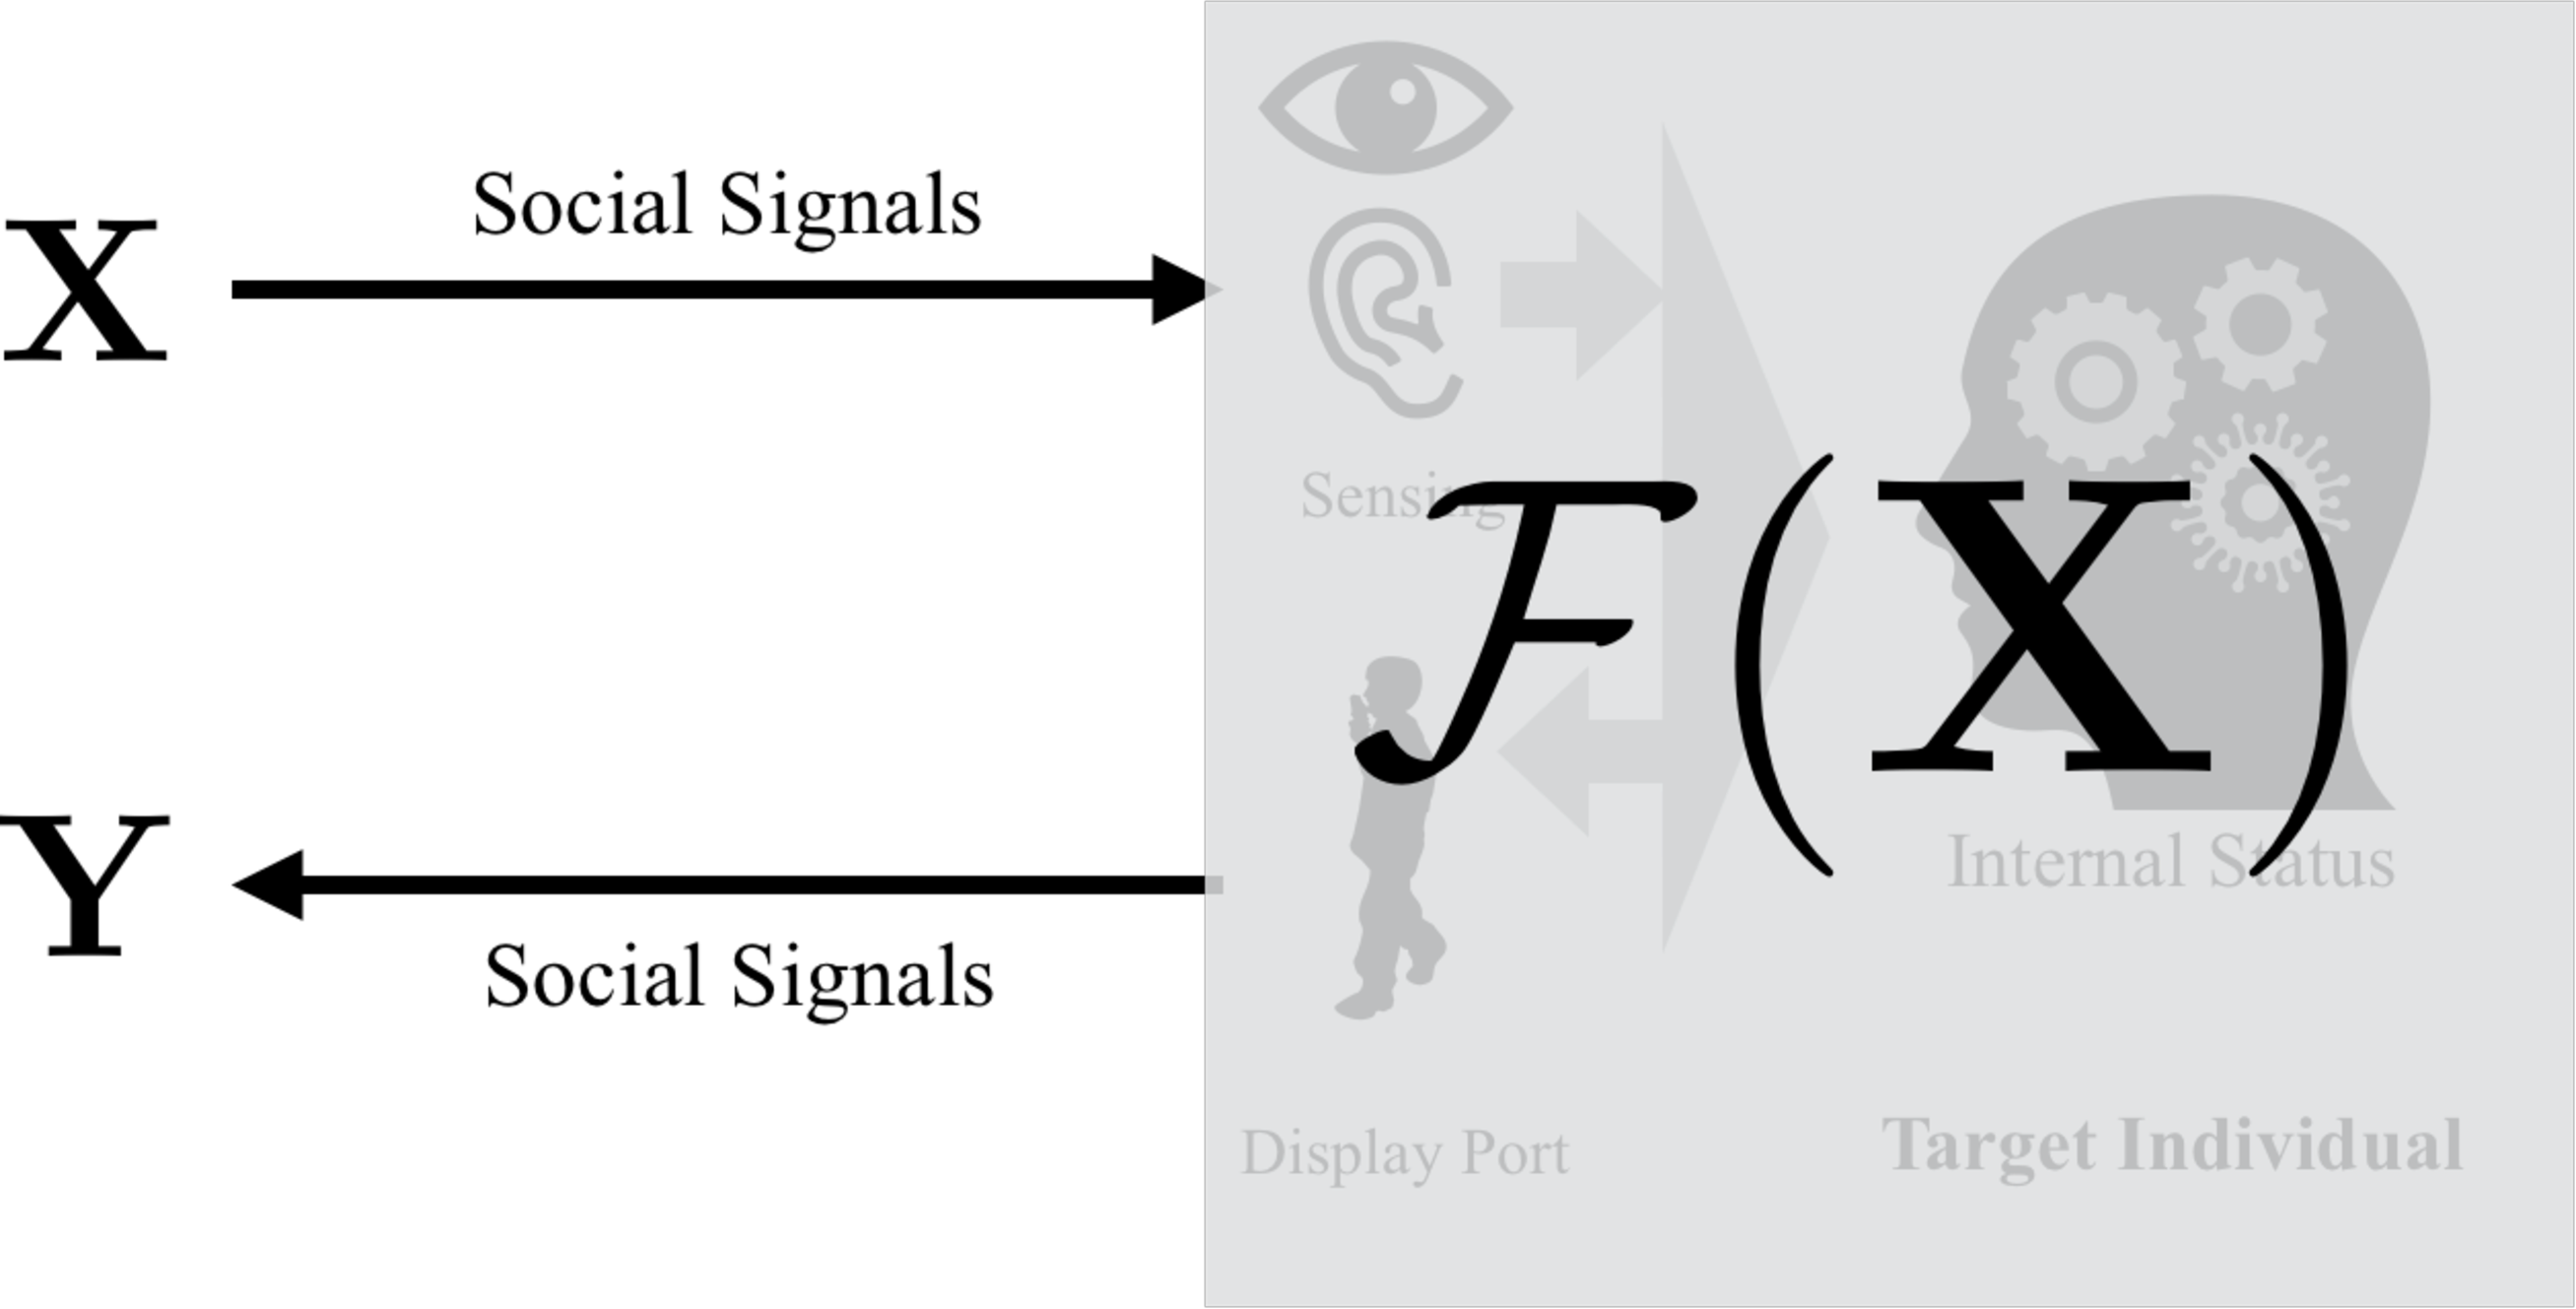
\includegraphics[width=\linewidth]{ssp_fig/ssp_def}
	\caption{We aim to build social artificial intelligence by building a model to learn the correlation between the input and output social signals. (Left) An example scene of RAPID-ABC test to detect autism spectrum disorder ~\cite{mathys2013beyond} and (Right) An illustration to describe social signal prediction task.}
	\label{fig:ssp_intro}
\end{figure}

% 1) We have 

% 2) General notations and social signal prediction problem. We formulate the prediction problem. 

% 3) We start from a simple signals. Proxemics and F-formation, and we make extension to more complicated signals, body and faces in social situation. We define the problem based on the difficulty. 

%     - position only
%     - body orientation (low freq.)
%     - face orientation
%     - body skeleton
%         - just better vis. from formation
%         - speaking / non-speaking (conditioned)
%         - social dynamics / social sync (nodding, synchrony, realistic?)
        
%     - Face/Hands
%         - just better vis. from formation + body
%         - speaking / non-speaking
%         - social dynamics / social sync (nodding, synchrony, realistic?)


% 5) We built a way to evaluate our method, as follows. 

% 1. L2 error
% 2. Classification error
% 3. Adding distribution and randomness (VAE?)

% 6) Conclusion and Future direciton




% Social interaction  long history but poor knowledge. Harder to define by manually defined models than language model. Language has grammar, what about nonverbal cues? We have seen the advance of language (and chatbot as the output). Limited measurment tool is the problem.  Language has tons of data in the web. No need to measure since verbal languages are directly mapped and recorded by letters. What about non verbal cues?

% A major advanced in facial expression (coding system, interaction). Body is limited, especially multi people's body, which are more commonly observable in our daily life. But vision made major advances. There exist robust tools. Now this problem is used in a practical level. We need to consider how to realize the social interaction model based on this tools. 


% However, It is not easy to computationally model social interaction. Extremely limited previous work. We may think it by using the analogy of language model or chatbot. We found (1) data is important, (2) nerual model is crucial. This paper presentned such direction for the first time. new DB can drive new research direction advances. MNist, Imagenet, 3D shapenet. 3D human DB, faceNet, and so on. 

% Thus, 

% 1) We have collected a sufficient amount of DB to study this assuming a specific (but still realistic) social situations. 

% 2) General notations and social signal prediction problem. We formulate the prediction problem. 

% 3) We start from a simple signals. Proxemics and F-formation, and we make extension to more complicated signals, body and faces in social situation. We define the problem based on the difficulty. 

%     - position only
%     - body orientation (low freq.)
%     - face orientation
%     - body skeleton
%         - just better vis. from formation
%         - speaking / non-speaking (conditioned)
%         - social dynamics / social sync (nodding, synchrony, realistic?)
        
%     - Face/Hands
%         - just better vis. from formation + body
%         - speaking / non-speaking
%         - social dynamics / social sync (nodding, synchrony, realistic?)


% 5) We built a way to evaluate our method, as follows. 

% 1. L2 error
% 2. Classification error
% 3. Adding distribution and randomness (VAE?)

% 6) Conclusion and Future direciton

% We start from indivdiual's multi modal signals, and show several noticeable component we can explore. 

% 4) Social formation. Simple but strong correlation among people which  well studied in previous work. We see wheather this social aspect can be learnt by machine. 

% Comparison to proxemics. 
% Evalution: body location, body orientation, face orientation. Orientation vs speaking GT?

% 5) More complicated singnals are studied. For example, body 2 body. However, the diverse is huge and motion are subtle, and less noticeable. So we focused on some cues by defining evalution tools. 


% Evalutation: How do we know it is working? Number may not be important. What else can we notices? It is hard, because we can feel but cannot define. 

% 1) Location + orientations 
% 2) orientation vs speaking
% 3) turn taking?

% 4) dynamics? nodding? Speed? human study?



\section{Related Work}

\textbf{Psychology:}
Due to its importance in social communication, nonverbal cues have received significant attention in psychology. Work in this area is often categorized into diverse subfields including Proxemics, Kinesics, Vocalics, and Haptics. In our work, we focus only on Proxemics and Kinesics, which are closely related to visual cues. Hall first introduced the concept of Proxemics to describe how humans use their personal space during communications~\cite{Hall66}, and Kendon studied the spatial formations and orientations established when multiple people communicate in a common space (named F-formation)~\cite{kendon90}. Facial expression in particular has received lots of attention by researchers since the pioneering work of Charles Darwin~\cite{Darwin-1872}. Ekman studied the relation between emotions and facial expressions, and presented Facial Action Code System (FACS) by introducing a system to describe facial expressions using combinations of atomic units (Action Units)~\cite{ekman1977facial}. Since then, this system remains as the de-facto standard to annotate and measure facial expressions, and has had a broad impact in across many fields. Compared to the face, body gestures remain relatively unexplored even though research has substantiated the importance of body language in communication~\cite{Gelder09, Moore13, Meeren-2005, Aviezer-2012}. In spite of the efforts of many researchers in diverse fields, little progress has been made in understanding nonverbal communications, and the approaches proposed several decades ago are still the most widely used methods available~\cite{Moore13}. %Especially the effort in understanding nonverbal communication  in pychology fields is rarely tranferred in building Artificial Intelligence communicating with humans.   

\textbf{Social Signal Processing:}
There has been increasing interest in studying nonverbal communication using computational methods~\cite{vinciarelli2009social, vinciarelli2012bridging}. Analyzing facial expression has been a core focus in the vision community ~\cite{ChuDC13, Torre15, shan2009facial}. Many other methods to automatically detect social cues from photos and videos have also been proposed, including F-formation detection~\cite{setti2015f}, recognizing proxemics from photos~\cite{yang2012recognizing}, detecting attention~\cite{Fathi-2012}, recognizing emotions by body pose~\cite{schindler2008recognizing}, and detecting social saliency~\cite{park20123d}. Affective computing fields has been growing up rapidly, where computer vision and other sensor measurements are used with machine learning technique to understand human's emotion, social behavior, and roles~\cite{picard1997affective}. 

\textbf{Forecasting human motion:}
Predicting or forecasting human motion is an emerging area in computer vision and machine learning. Researchers propose approaches for predicting pedestrian's future trajectory~\cite{kitani2012activity} or forecasting human interaction in dyadic situations~\cite{huang2014action}. More recently, deep neural network are used to predict future 3D poses from motion capture data~\cite{mnih2012conditional, Fragkiadaki_2015_ICCV, jain2016structural}, but they focus on periodic motions such as walk cycles. Recent work tries to forecast human body motion in the 2D image domain~\cite{walker2016uncertain, villegas2017learning}. A few works address trajectory prediction in social situations~\cite{helbing1995social, alahi2016social, gupta2018social}. 

%Holden's work
%Graphics Jehee's
%Sergey Levin's work
%
%\textbf{Social Signal Dataset:}
%How to measure and collect nonverbal signal data is important to pursue a data-driven approach for our goal. However, only few datasets contain socially interacting group motion~\cite{alameda2016salsa, mccowan2005ami, lepri2012connecting, rehg2013decoding}. The scenes in these datasets are often in a table setup, limiting free body movement and capturing the upper-body only. There are datasets that capture more freely moving multiple people (e.g., cocktail party)~\cite{Zen-10, Cristani-11, farenzena2009social}, but these only contain location and orientation measurements for the people, introduced to study the social formation only. Datasets providing rich 3D body motion information captured with motion capture techniques exist, but they contains single subjects' motion only\cite{gross2001cmu, h36m_pami, sigal2010humaneva}. More recently, however, full body motion data of interacting groups using a large number of camera system was proposed for social interaction capture~\cite{Joo-15}. This work shows a potential in collecting a large scale social interaction data without the usual issues caused by wearing a motion capture suit and markers.

\textbf{Measuring Nonverbal Signals in Imagery:} Detecting human bodies and keypoints in images has advanced greatly in computer vision. There exist publicly available 2D face keypoint detectors~\cite{baltruvsaitis2016openface}, body pose detectors~\cite{cao2017realtime, Wei2016, Newell-16}, and hand pose detectors~\cite{simon2017hand}. 3D motion can be obtained by markerless motion capture in a multiview setup~\cite{Gall-09,Liu-2013,Elhayek-15, joo2017panoptic, joo2018}, by RGB-D cameras~\cite{Shotton2011,Baak2011}, or even by monocular cameras~\cite{Ramakrishna2012,Bogo2016,martinez2017simple,zhou2017towards,Moreno-noguer2017,mehta2017monocular}. Recently, methods to capture both body and hands have also been introduced~\cite{MANO:SIGGRAPHASIA:2017,joo2018}. 

% !TEX root = thesis.tex


\section{Social Signal Prediction}
The objective of \emph{Social Signal Prediction} is to predict the behavior of a target person in a social situation. The target person's behavior is correlated to the social situation. For example, the location and orientation of the target person should be strongly affected by the position of conversational partners (known as Proxemics~\cite{Hall66} and F-formation~\cite{kendon90}), and the gaze direction, body gestures, and facial expressions of the target person should also be ``conditioned" by the behaviors of the conversational partners. In the social signal prediction task, we model this conditional distribution among interacting subjects, to ultimately teach a robot how to behave in a similar social situation driven by the behavior of communication partners. There exist cases where the correlation of the social signals among subjects is strong, such as hand-shaking or greeting (waving hands or bowing). But in most of the cases, the correlation is implicit---there exists no specific rules how to behave given other people's behavior, which makes it hard to manually define the rules. In our approach, we tackle this problem in a data-driven manner, by automatically learning the conditional distributions using a large scale multimodal social signals corpus.  

Let us denote all types of signals that the target person received in a social situation at time $t$ as $\mathbf{X}(t)$. Thus $\mathbf{X}(t)$ includes the social signals---body gestures, facial expression, body position, voice tones, verbal languages---and other contextual factors such as the space where the conversation is performed or other visible objects which may affect the behavior of the target person (e.g., some sounds or objects may attract the attention of the person). We divide the inpu signal $\mathbf{X}(t)$ into two parts, the signals from the conversational partners, $\mathbf{X}_c(t)$, and signals from other sources (e.g., objects, environment, and other human subjects not interacting with the target person), $\mathbf{X}_e(t)$.  Thus,
\begin{equation}
\mathbf{X} (t) = \{  \mathbf{X}_c (t), \mathbf{X}_e (t)\}.
\end{equation}
The $\mathbf{X}_c (t)$ may contain social signals from multiple people and we denote the signals from each subject separately:
\begin{equation}
\mathbf{X}_c (t) = \{ \mathbf{X}_c^i (t) \}_{i=1}^N,
\end{equation}
where $\mathbf{X}^i_c (t)$ are the signals from the $i$-th conversational partner in the social interaction and $N$ is the total number of partners. 
Similarly, we denote the signals emitted by the target person at time $t$ in the socials situation as $\mathbf{Y} (t)$.
The goal of social signal prediction is to find a function $\mathcal{F}$ which takes $\mathbf{X}$ as input and produces $\mathbf{Y}$ as output to mimic the behavior of the target person in the social situation:
\begin{equation}
\mathbf{Y} (t+1) = \mathcal{F} \left( \mathbf{X} (t_0:t), \mathbf{Y} (t_0:t) \right),
\label{equation:socialPrediction_1}
\end{equation}
where $t_0:t$ represents a range of time from $t_0$ to $t$ affecting the current behavior of the target person. Note that we define the function $\mathcal{F}$ to take the history of the target person's own signals $\mathbf{Y} (t_0:t)$. Intuitively, this formulation models the human behavior as a function that maps the correlation among social signals the target person receiving and emitting. The function can be defined for a specific individuals, representing the personal behavior of the target person encoding characteristic, gender, and culture of the target. Based on that, different individuals may behave differently. If the function is regressed by data of many people, then we hypothesize that the function produces more general and common social behaviors, where the person's specific behaviors are averaged out.

Previous approaches can be considered as subsets of this model. For example, conversational agents (or chatbots) using natural language only can be represented as:
\begin{equation}
\mathbf{Y}_v (t+1) =  \mathcal{F} \left( \mathbf{X}_v (t_0:t) \right),
\end{equation}
where $\mathbf{Y}_v$ and $\mathbf{X}_v$ represents only verbal signals. The human motion forecasting studied in computer vision and graphics~\cite{Fragkiadaki_2015_ICCV, jain2016structural} can be considered as:
\begin{equation}
\mathbf{Y}_n (t+1) =  \mathcal{F} \left( \mathbf{Y}_n (t_0:t) \right),
\end{equation}
where $\mathbf{Y}_n$ represents only non-verbal motion capture. Note that in this task, there is no social interaction modeling, and the prediction is only for an individual using their own previous signals. 

In our work, we focus on non-verbal social signal prediction in a triadic social interaction in the Haggling game scenario:
\begin{equation}
\mathbf{Y} ( t_0:t ) =  \mathcal{F} \left( \mathbf{X}^1 (t_0:t), \mathbf{X}^2 (t_0:t) \right),
\label{equation:F_ours}
\end{equation}
where we predict the social signals of the target person given the signals of the two other people during the same window of time. %Modeling rich non-verbal socials (e.g., body motion) among interacting multiple people (more than two) has been rarely studied in previous work.

%What signal?

% \section{Predicting Social Signals in a Tridadic }






% emitted from the target person at time $t$ are represented as $\mathbf{U} (t)$. Here, we define $\mathbf{U} (t)$ to include verbal signal $\mathbf{U}_v (t)$ and nonverbal signals $\mathbf{U}_n (t)$, 





% for example


% responding other people's social signals (either same window of time or future). The signal is not arbitrary but should have a strong correlation with the signals the person transmitted and received. Let us assume that all types of signals emitted from the target person at time $t$ are represented as $\mathbf{U} (t)$. Here, we define $\mathbf{U} (t)$ to include verbal signal $\mathbf{U}_v (t)$ and nonverbal signals $\mathbf{U}_n (t)$, 
% % and even non-measurable internal ``signals" of the person, $\mathbf{x}_{\omega} (t)$, such as feeling, emotions, thought, belief, religion, knowledge and so on, which can affect the future motion of the target person\footnote{Such non-measurable signals can only be ``measurable" by the target person oneself.}.
% \begin{equation}
% 	\mathbf{U} (t) = \{  \mathbf{U}_v (t), \mathbf{U}_n (t)\}.%, \mathbf{x}_{\omega} (t) \}
% \end{equation}

% We also define the signals $\mathbf{V}(t)$ originated from outside and received (or sensed) by the target person. This signals contains verbal $\mathbf{V}_v (t)$ and non-verbal signals $\mathbf{V}_n (t)$,
% \begin{equation}
% \mathbf{V} (t) = \{  \mathbf{V}_v (t), \mathbf{V}_n (t)\}.%, \mathbf{y}_{e} (t) \}. 
% \end{equation}


% We denote the signals emitted from non-human environment  $\mathbf{E}(t)$ that affects the target person's future motion. For example, the existence a chair induce the person to sit on it, and existence of roads makes the person to walk on it. Note that both $\mathbf{U}$ and $\mathbf{E}$ should be measurable by the target person's sensing system, otherwise the signals do not affect to the target person's future motion. We ignore all the non-sensible signals (e.g., infrared light and ultra sound).

% During social communications, humans use all the current and previous information to make a future decision. Similarly, Social Signal Prediction should take into account all the observed signals up to the time to predict the future signal $\mathbf{U} (t+1)$. The goal of Social Signal Prediction is to regress a function $\mathcal{F}$ defined as:
% \begin{equation}
% \mathcal{F} \left( \mathbf{U}  (t_0:t),   \mathbf{V} (t_0:t), \mathbf{E}(t_0:t) \right) = \mathbf{U} (t+1),
% \label{equation:F}
% \end{equation}
% where $\mathbf{U}(t_0:t)$, $\mathbf{V} (t_0:t)$, and $\mathbf{E} (t_0:t)$ represent signals from $t_0$ to $t$, and the $t_0$ denotes the very initial time that the target person transmits/receives any signals (his/her birth). 

% Intuitively, $\mathcal{F}$ model how to react in future considering all the input the person has observed from outside and by oneself. In non-social situations where the person is alone ($\mathbf{V(t)}=\phi$), the future motion is mainly dependent to the person's own status and environments. For example, we can predict that a pedestrian will keep walking on the road, because of the ``walking" signals in $\mathbf{U}(t-w:t)$ and existence of road signal in $\mathbf{E}(t-w:t)$, where $t-w$ is the recent past time. In social communication situation, $\mathcal{F}$ produces output as an reaction of other people's signals. For example, making a certain distance from the location of other people, listening when other people are speaking, and speaking when other people are listen (turn taking), facing each other, and so on. $\mathcal{F}$ can be affected by the input from a long-term history, reflecting the person's culture, education, and personality. Depending on it, each person may react differently given the same current signals. 

% In practice, it is infeasible to train the Equation~\ref{equation:F} with all the data from one's birth. However, we hypothesize there exist many nonverbal communication protocols that is dominantly dependent to current and near past signals, and commonly performed by people. Additionally, we further assume that we can ignore $\mathbf{E}$ by only considering the scenes to minimize this, and also ignore verbal signals to only focus on nonverbal cues. In this work, we consider the following equation, 
% \begin{equation}
% \mathcal{F} \left( \mathbf{U}_n  (t-w:t), \mathbf{V}_n (t-w:t) \right) =\mathbf{U}_n (t+h).
% \label{equation:F_ours}
% \end{equation}
% Note that we try regress the function to predict a future time $t+h$ where $h$ is a horizon we are interested in. 

% There are two issues to be discussed here. First, we assume that $\mathbf{U}$ and $\mathbf{V}$ only contain social signals already ``precessed" from raw data. For example, raw signals are sensed by human by sensing system (e.g., videos from eyes and audios from ears), and they are interpreted by a perception system as body gestures and facial expressions. To focus on the social signal prediction itself, we assume that the input of the Equation \ref{equation:F_ours} is already processed by computer vision algorithms. Second, the level of richness of the input signals should affect the prediction performance. Ideally, all the signals that are measurable by human should be considered. However, there still exists several challenges in machine perception methods. In this paper, we use measurement nonverbal signals (3D body and face landmarks) obtained by the-state-of-the art computer vision system  and more focus on the impact of $V$ compared to the case using $U$ alone.

% \subsection{Notations for Social Signals}

% In this section, we formally define the notation of $\mathbf{U}(t)$ and $\mathbf{V}(t)$ of Equation~\ref{equation:F_ours}. We consider multiple tasks by considering different type of $\mathbf{U}(t)$ and $\mathbf{V}(t)$. In our experiment, we use location and orientation as the simplest signal types (considering social formations), and full 3D body and face landmarks as the richest signals. 

% \textbf{Root location/orientation}:	We consider a 3D point and an angle to represent a person's location and orientation. These can be defined based on either face or upper body. In either case, we choose a root landmark and extract a normal direction using cross product among three selected landmarks, as shown in Figure~\ref{fig:bodyFaceNormals}. We denote $\mathbf{x}_i(t) \in \mathbb{R}^3$ to represent the location of $i$-th person in the world coordinate at time $t$. $\mathbf{x}_i(1:t) \in \mathbb{R}^{3 \times t}$ is a row vector by concatenating root locations from time $1$ to $t$ of the $i$-th person. The differential of locations, $\Delta \mathbf{x}_i(t) = \mathbf{x}_i(t+1) - \mathbf{x}_i(t) \in \mathbb{R}^3$, represents a location change in subsequent frames at world coordinate. Orientation is represented only w.r.t. $Y$ axis using a single scalar angle value, similar to ~\cite{mnih2012conditional, Fragkiadaki_2015_ICCV}. The orientation of $i$-th person $\theta_i(t) \in \mathbb{S}$ is computed by projecting the normal vector on XZ plane and computing the counter-clockwise angle from positive X axis. From this angle, we can deterministically compute a rotation matrix $\mathbf{R}_i(t)$ w.r.t. $Y$ axis, which transforms the coordinate from world to the person-centric views. We also consider its concatenation as $\theta_i(1:t) \in \mathbb{S}^{t}$, and its differential, $\Delta \theta_i(t) = \theta_i(t+1) - \theta_i(t) \in \mathbb{S}$.

% 	The location defined in the global coordinate system can be transformed to a person centric coordinate system. The $i$-th subject's location in $j$-th person centric coordinate system at $t$ is represented as,
% 	\begin{equation}
% 	\mathbf{x}^{j,t_j}_i(t) = \mathbf{R}_j(t_j) \left( \mathbf{x}_i(t) - \mathbf{x}_j(t_j)  \right)  + \mathbf{x}_j(t_j).
% 	\label{eq:personCentric}
% 	\end{equation}
% 	Note that we allow to consider different times for $i$-th and $j$-th person in this equation ($t$ vs $t_j$). Using this notation, we can compute the location at $t+1$ in the its own person-centric coordinate at time $t$,
% 	\begin{equation}
% 	\mathbf{x}^{i,t}_i(t+1) = \mathbf{R}_i(t) \left( \mathbf{x}_i(t+1) - \mathbf{x}_i(t)  \right)  + \mathbf{x}_i(t)
% 	\end{equation}
% 	The differential of locations in the person-centric coordinate system is represented by 
%   \begin{gather}	
% 	\Delta \mathbf{x}^{i}_i(t) = \mathbf{R}_i (t) \left( \mathbf{x}_i(t+1) - \mathbf{x}_i(t)  \right) ) =  \mathbf{R}_i (t)\Delta \mathbf{x}_i(t)
% 	\end{gather}
% 	Similarly, we can consider the differential of the $i$-th person in $j$-th person's coordinate system. 
%   \begin{gather}	
%   \Delta \mathbf{x}^{j}_i(t) = \mathbf{R}_j (t) \left( \mathbf{x}_i(t+1) - \mathbf{x}_j(t)  \right) ).
%   \end{gather}	
% 	This representation is less intuitive because it mixes two type of differentials, between times ($t$ and $t+1$) and a relative social formation between $i$-th and $j$-th person. We found, however, that this representation works better in modeling social signals. 
% 	The differential of orientation in the person centric coordinate system is the the same as in world coordinate, $\Delta \theta_i(t) = \Delta \theta^j_i(t)$, because $\theta$ is a scalar value.

% 	\textbf{Body skeleton}:  In this paper, joint landmarks at a time $t$ is always considered in a person-centric coordinate system by decoupling global translation and orientations, using the Equation~\ref{eq:personCentric}. Each $k$-th body landmark of $i$-th person a $t$ is represented by the relative unit direction w.r.t. the parent joint landmarks:
% 	\begin{equation}
% 	\mathbf{j}_i(k, t) = \frac{\gamma_i(k, t)  -  \gamma_i ({p(k)}, t)} {|| \gamma_i (k, t)  -  \gamma_i (p(i),t)  ||_2}
% 	\end{equation}
% where $\gamma_i (k,t) \in \mathbb{R}^3$ represents the $k$-th landmark location of person $i$ at $t$ in the person-centric coordinate, and $p(k)$ is the index of the parent landmark of $k$-th joint. So, $\mathbf{j}_i$ is a unit vector representing the bone direction by canceling out bone length information of the person. We also consider a row vector concatenating all joints, $\mathbf{j}_i(2:15, t)$ (from joint 2 to 15). We ignore the first joint because it is the root defined above.

% 	\textbf{Face landmark}: 53 facial landmarks are generated by the system. To reduce the dimension, we run PCA, and reduce the dimension to 20 variables, $ \eta_i(t) \in \mathbb{R}^{20}$. This particular dimension is chosen to maintain XX percents of the variation in the face. 

% 	\textbf{Face and body connection}: In practice, the face landmarks are rigidly linked to the body skeletons. We connect face to body using an extra connection from head top to the face center (nose top). This additional joint is also represented in the same way as other body joint and denoted as $\mathbf{j}_i(k_f,t) \in \mathbb{R}^3$, where $k_f$ means the joint index for face. % and determines the location and orientation of the face.
% %		
% %			
% %	  Vector concatenation of root orientations of subject $i$  from time $1$ to $t$\\
% %	
% %	
% %	To compute this we project normal vector on t Orientation w.r.t. Y-axis of subject $i$ at time $t$\\
% %			
% %	in a 2D space ignoring Y axis (height).  We extract the location and orientation data from the reconstructed faces.  \\
% %	
% %	 As a measured signal we consider 3D face and 3D body as the  landmarks as nonverbal signals, to represent coherent  
% %	
% %	 represents 3D face and body landmarks. There can be diverse variation about how to model this. Important concept is how to normalize, represent the data to keep better coherency. This is related to ``invariance" of the data. Such as person-invariant, location-invariance. and so on. 
% %	
% %
% %	
% %	\noindent
% %	$\mathbf{x}_i(t) \in \mathbb{R}^2$:  location in the world coordinate of subject $i$ at time $t$\\
% %	$\mathbf{x}_i(1:t) \in \mathbb{R}^{2 \times t}$: Vector concatenation of root locations of subject $i$ from time $1$ to $t$\\
% %	
% %	$\Delta \mathbf{x}_i(t) = \mathbf{x}_i(t+1) - \mathbf{x}_i(t) \in \mathbb{R}^3$: location changes in world coordinate\\
% %	$\mathbf{x}^{j}_i(t) = \mathbf{R}_j(t) \left( \mathbf{x}_i(t) - \mathbf{x}_j(t)  \right) )\in \mathbb{R}^3$: location changes between time $t$ and $t+1$ in the person-centric coordinate of subject $j$ at time $t$. $\mathbf{R}_j(t)$ is a rotation matrix to transform from world coordinate to the person-centric coordinate of subject $j$ \\
% %	$\Delta \mathbf{x}^{j}_i(t) = \mathbf{x}^{j}_i(t+1)  - \mathbf{x}^{j}_i(t)$\\  
% %	$=  \mathbf{R}_j(t+1) \left( \mathbf{x}_i(t+1) - \mathbf{x}_j(t+1)  \right) ) - \\ 
% %	\quad \quad \mathbf{R}_j(t) \left(  \mathbf{x}_i(t) - \mathbf{x}_j(t)  \right) )    \in \mathbb{R}^3$: 
% %	location changes between time $t$ and $t+1$ of subject $i$ in the person-centric coordinate of subject $j$ at each corresponding time. Intuitive, the value represents changes in relative location between the subject $i$ and $j$   \\
% %	
% %	
% %	\noindent
% %	$\theta_i(t) \in \mathbb{S}$:  Orientation w.r.t. Y-axis of subject $i$ at time $t$\\
% %	$\theta_i(1:t) \in \mathbb{S}^{t}$: Vector concatenation of root orientations of subject $i$  from time $1$ to $t$\\
% %	$\Delta \theta_i(t) = \theta_i(t+1) - \theta_i(t) \in \mathbb{S}$: orientation changes in world coordinate\\
% %	$\Delta \theta_i(t) = \Delta \theta^j_i(t)$: orientation changes in a person-centric is the same as the changes in world coordinate (since the values is a scalar)\\
% %	
% %	%Body joint representation
% %	We represent body using the relative location of joint w.r.t parent joint. The method of Joo et al produces only joint locations without angles. To make the representation independent from person identity and global orientation, we first decouple global root motion from the original coordinate system, and represent joint in the person centric coordinate system. And we also normalize the distance and only keep the directional vector to the joint from its parent joint. 
% %	
% %	\begin{equation}
% %	j_1(i)  = R_{w1} (t) \dot 	( j_w(i) - j_w(i_p))
% %	\end{equation}
% %	
% %	
% %	%Face
% %	Face dimension is reduced by PCA. Original dimension is $53\times3$ but it doesn't have much variation. After PCA, we only use 20 dimensition to represent variabtion of face from the mean face. 
% %	
% %	In our results, we shows that different representation also affect the learning performance. 
% %	%	$\mathbf{J}_i(k,t) \in \mathbb{R}^{3}$: $k$-th joint representation of subject $i$ w.r.t. parent joint in person centric coordinate system (after canceling out root location and orientation). $|| \mathbf{J}_i(k,t) ||=1$\\
% %	%	$\mathbf{J}_i(1:k,t) \in \mathbb{R}^{3}$: Vector concatenation of joint 1 to $k$
% !TEX root = thesis.tex

\section{Triadic Interaction Dataset with Full-spectrum Social Signal Measurements}
%\label{section:dataset}
%Availability of a large-scale dataset is essential to tackle the social signal prediction task in a data-driven way. Despite existing datasets that provide measurements for human motion and behaviors~\cite{carletta2005ami, Lepri-12, Zen-10,Cristani-11, SALSA-15, h36m_pami}, there is no dataset that satisfies the following core requirements for understanding non-verbal human behaviors: (1) capturing 3D full body motion at high-resolution (including face, body, and hands); (2) capturing signals of naturally interacting groups (more than two people to include attention switching); and (3) collecting the data at scale. The limited availability of the dataset motivates us to build a new dataset that contains social interactions among hundreds of interacting groups with the full-spectrum of 3D body motion measurements. The key properties of our dataset are as follows:
%\begin{itemize}
%	\item Our dataset contains naturally interacting multiple people in a negotiation game scenario that is carefully designed in the collaboration with pychologists
%	\item No behavioral restriction is instructed to participants during the capture, and subjects are randomly recruited
%	\item Our dataset contains videos from over 500 views. All cameras are calibrated and temporally synchronized
%	\item High-resolution social signals are measured using markerless motion capture~\cite{joo2017panoptic, joo2018}, including 3D anatomical landmarks for body, face, hands, and 3D point clouds
%	\item Our dataset contains audio recording the voice signal for each subject, which is synchronized with videos, as well as annotated speaking status for each individual
%\end{itemize}

The objective of our dataset is to study the correlation among subtle socials signals transmitted during a social situation. To make human behaviors more coherent, we define a social scenario so that all the subjects are in the same social situation. Capturing the natural motion of the subjects is crucial in our study, so we use the state-of-the art markerless motion capture methods in the CMU Panoptic Studio~\cite{joo2017panoptic, joo2018}. Importantly, the multi-modal property of our dataset enables us to study the correlation among various input and output signals. Our dataset is captured under a university-approved IRB protocol and will be publicly available for research purposes.
\begin{figure}
	\centering
	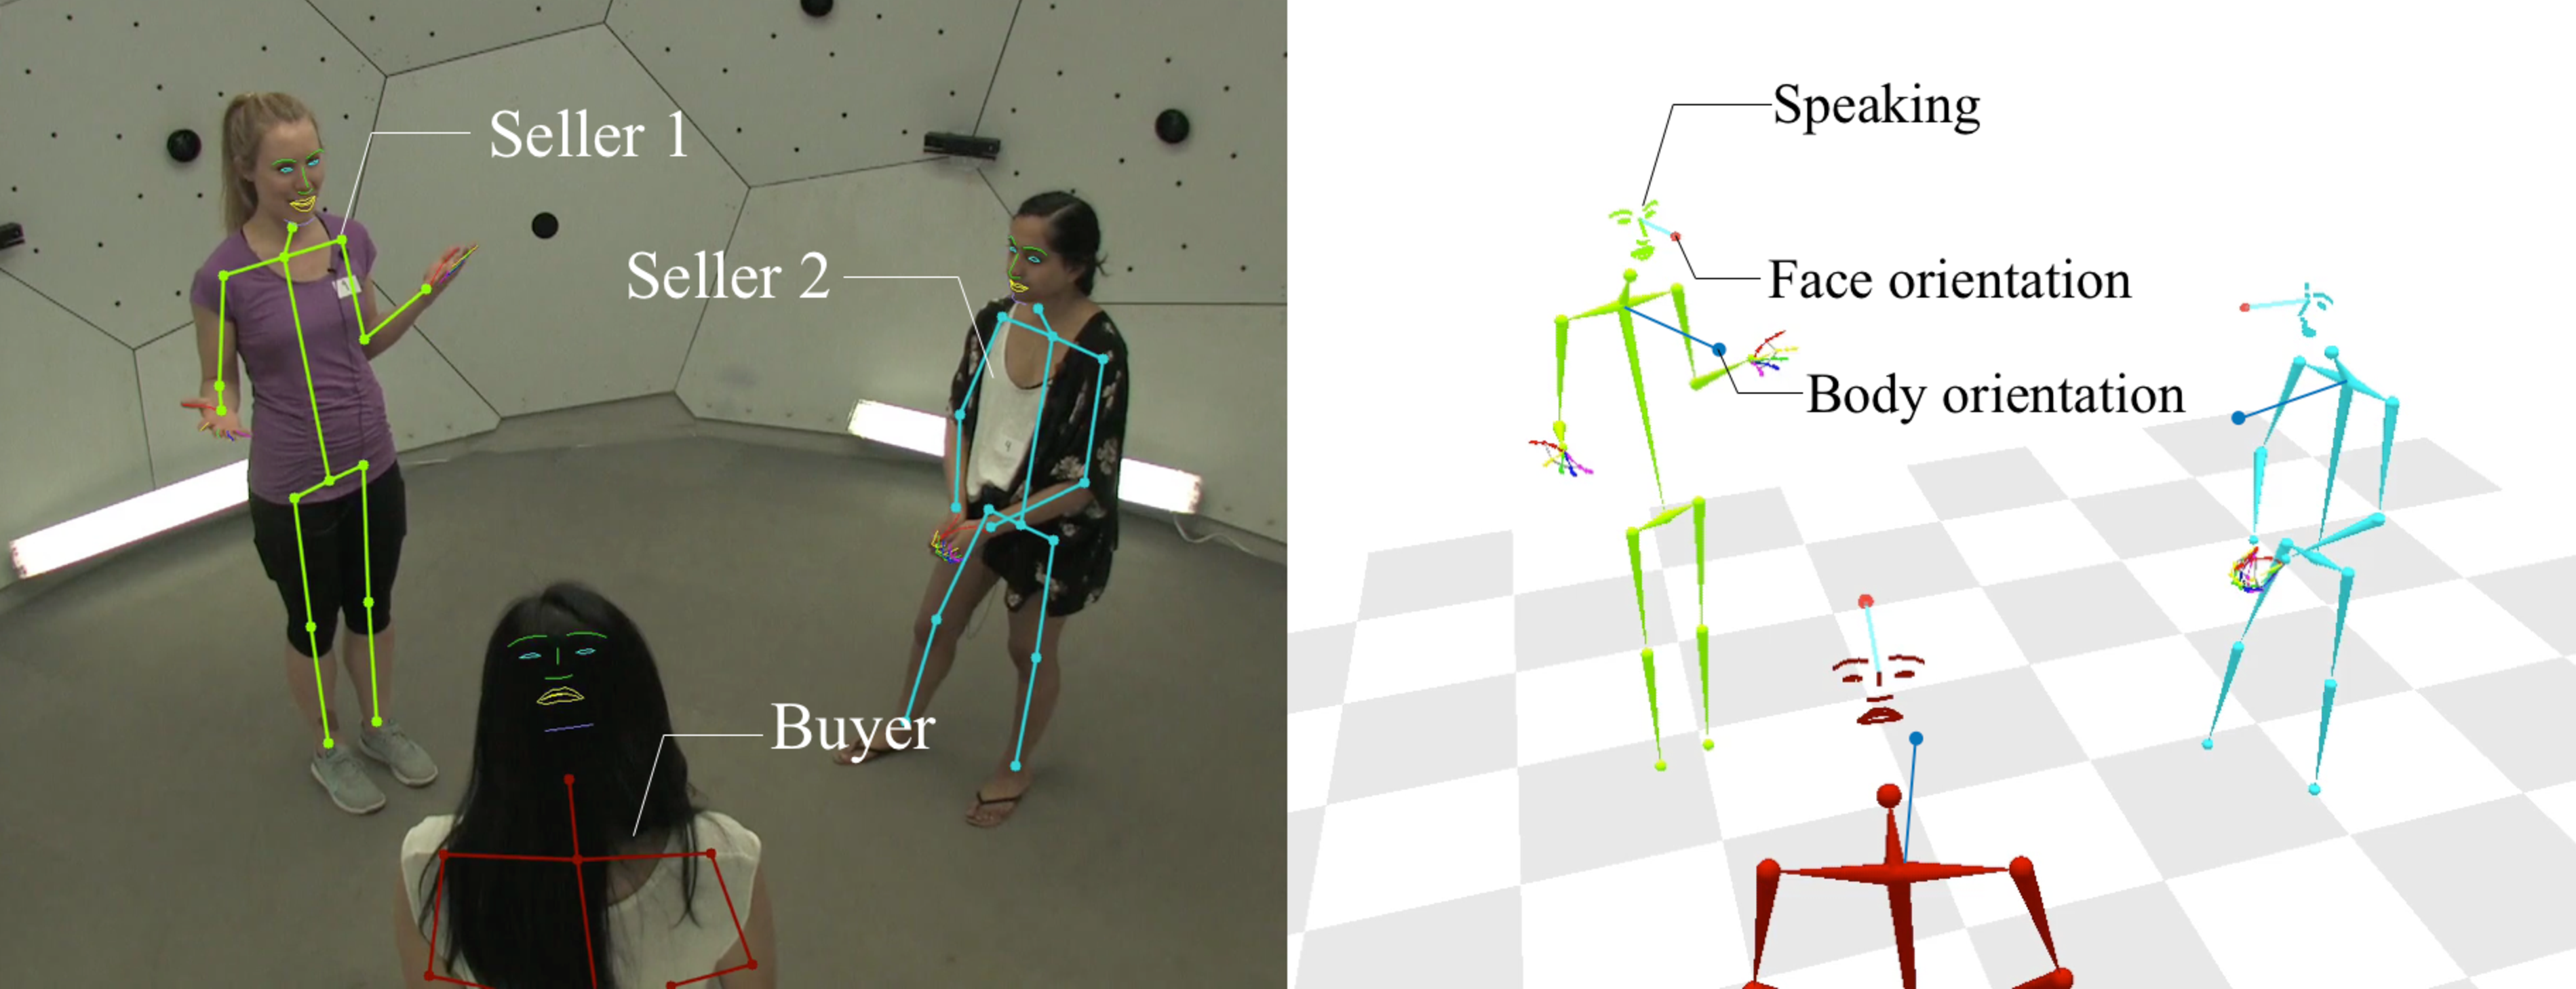
\includegraphics[width=\linewidth]{ssp_fig/haggling_ex}
	\caption{An example of the haggling sequence. (Left) an example scene showing two sellers and one buyer. (Right) Reconstructed 3D social signals showing body, face, and 3D hand motion.} 
	\label{fig:hagglign_ex}
\end{figure}

% We use the state-of-the-art markerless motion capture method to measure the full spectrum of social signals including 3D keypoint from body, face, hands, and foot~\cite{joo2017panoptic, joo2018}. Since this method does not require any sensor attachement on subject's body or other types of initialization asked for the subject during the capture, it can capture natural body behaviors of the interaction. 
%
%\subsection{The Haggling Game Protocol}
%To evoke natural interactions, we involved participants in a social game named the \emph{Haggling} game. This game induces a variety of rich non-verbal signals in participants. In our captures, subjects were informed of the rules of the game but were otherwise not instructed about how to behave, nor was their clothing or appearance controlled. They were also not initially aware of our research goals to avoid potential biases in their gestures. The majority of the sequences are captured with people randomly recruited from a university campus. We invent this haggling game to simulate a haggling situation among two sellers and a buyer. The triadic interaction is chosen to include interesting social behaviors such as turn taking, and attention changes, which are missing in dyadic interactions~\cite{rehg2013decoding}. During the game, two sellers are promoting their own comparable products for selling, and a buyer makes the decision about which product he/she buys between the two. They are given a minute for the haggling, and the seller who has sold his/her product is awarded $\$5$. To maximize the influence of each seller's behavior on the buyer's decision-making, the items assigned to sellers are the same type of product with slightly different properties. We provide simple written descriptions to sellers about the items 1 minute before the game. Over the 8 days of captures, 122 subjects participated and 180 haggling sequences were captured (about 3 hours data). The captured sequences contain a lot of voluntary social behaviors of diverse people in a common social context (an example scene is shown in Fig.~\ref{fig:hagglign_ex}. Note that the capture space does not contain other objects which may distract the motion of the target, so we can assume no $X_e(t)$ is necessary in our social signal prediction problem.

%\subsection{Measuring Social Signals}
We use the Panoptic Studio System to reconstruct 3D anatomical keypoints of multiple interacting people~\cite{joo2017panoptic, joo2018}. As a key advantage, the method does not require attaching sensors or markers on subject's body, and no behavior restrictions nor initialization poses are needed from the subjects. As output, the system produces 3D body motion $\mathbf{J(t)}$, 3D face motion $\mathbf{F(t)}$, and 3D hand motion $\mathbf{H(t)}$ for each individual at each time $t$. From this measurement, we additionally compute the body orientation $\theta(t)$ and face orientation $\phi(t)$ by finding the 3D normal direction of torso and face. These orientations are computed only on the $x$-$y$ plane with respect to the $y$-axis. We decouple the global location $x$ and body orientation $\theta$ from the body motion capture results, following previous work~\cite{jain2016structural, holden2016deep}, and $\mathbf{J(t)}$ only contains body motions in the person-centric coordinate (root joint is at the origin and body is facing the $z$ direction). An example scene is shown in Fig.~\ref{fig:hagglign_ex}. The voice data $V(t)$ of each individual is also recorded by wireless microphones assigned to each individual. From the audio signal, we manually annotate a binary speaking label $\mathbf{S}(t) \in \{0,1\}$ describing whether the target subject is speaking (labelled as $1$) or not speaking (labelled as $0$) at time $t$. In summary we measure the following signals for each individual:
\begin{equation}
[ \mathbf{x}, \boldsymbol{\theta}, \boldsymbol{\phi}, \mathbf{J}, \mathbf{F}, \mathbf{H}, \mathbf{V}, \mathbf{S} ].
\label{equation:measurement}
\end{equation}


% 사람과 같이 행동하는 기계를 만드는 것은 AI와 Robot을 연구하는 모든 사람들의 목표일것이다.  무엇이 사람을 사람답게 만드는가? 특별히 다른 사람들과 의사소통을 하는 능력은 사람을 다른 생물들과 차별시키는 주요한 특징 중에 하나일것이다. 이 논문에서는 인간의 여러가지 특성중 다른 사람과 상호작용하는 능력에 대해 주목한다.  

% 사람과 같이 의사소통을 하는 로봇에 관한 연구는 전혀 새로운것이 아니다. 이미 HCI, HRI, social robotics, AI 등 광범위한 범위에 걸쳐서 이 분야가 연구되고 있다. 하지만 아직까지 실제로 사람과 같이 의사소통을 하는 머신은, 혹은 그렇게 하고 있다고 여겨지는 머신은, 아직 만들어지지 못했다. 그럼 이것이 왜이렇게 어려운 문제이며, 이것을 해결하기 위해서는 어떤 해결책을 모색해야하는걸까?

% 이것을 이야기하기 위해서, 우리는 먼저 "의사소통을" 하는 사람들의 행위에 대해서 다시 한번 생각해볼 필요가 있다. 사람이 의사소통을 한다는것은 과연 무엇일까? 한가지 예를 들어보자. 두명의 사람이 있다. 그 두사람이 대화를 하고 있다고 하자. 우리는 아주 쉽게 이 둘이 대화를 하고 있는지 아닌지를 구분할 수 있다. 이같은 판단을 내릴 수 있는 이유는 무엇인가? 의사소통하지 않는 두명의 모습을 모여줄때랑, 의사소통을 하는 두 사람의 모습을 보여줄때, 한쪽은 커뮤니케이션 중이며, 다른쪽은 아니라는것을 우리는 과연 어떤 기준으로 쉽게 판단할수 있는가? 만일 이것을 쉽게 판단할 수 있는 어떤 규칙을 우리가 발견할수 있다면, 의사소통을 하는 로봇을 만드는 방법은 꽤 간단할 수 있다. 바로 그 규칙을 따르도록 로봇을 만들면 된다. 

% 자, 그럼 이제 의사소통을 하는 사람들의 특징이나 패턴에 대해 한번 생각해보자. 이것또한 새로운 연구주제가 아니다. 이미 아주 오래전부터 pychology 에서 연구되고 고민되는 문제이다. 이 예전 work 들을 들여다보기 전에, 사람의 의사소통이라는게 과연 어떤 목적으로 이루어지는지를 한번 고민해보는게 도움이 될것이다. 

% 사람은 왜 의사소통을 하는가? 바로 서로의 생각과 의견을 주고 받기 위함이다. 우리는 우리 생각을 공유하기 위해 말을 사용하고, 표정을 사용하고, 몸짓, 그리고 모든 미묘한 사람의 몸에서 만들어지는 큐들을 사용한다. 때로는 우리가 굳이 주고받지 않으려고 하는 내용조차도 다른 사람에게 자연스럽게 노출이 되는경우도 있다. 그냥 가만히 무표정하게 서있는다거나, 무의식적으로 몸을 움직인다거나, 그러니까 우리가 의도하고 보내든 그렇지 않든, 우리는 어떠한 형태의 "시그널"을 다른 사람에게 보내고 이 "시그널"은 다른 사람에게 어떤 형태의 메세지를 전달한다. 이 메세지는 언어로 설명할수 있는 레벨이 있을수 있고, 언어를 초월하는 어떤 느낌이나 의도 등의 것들일 수 도있다. 한편으로는 사람의 커뮤니케이션은 기계들의 커뮤니케이션과 유사하다. 이 커뮤니케이션 형태를 통해 어떤 정보가 교환된다. 한가지 큰 차이점은, 기계의 커뮤니케이션에서는 통신을 위한 프로토콜 (이를테면 데이터를 encoding/decoding 하는 규칙) 이 미리 잘 정의되어있지만, 사람의 통신에서는 그것이 아직 명확하게 정의되고 있지는 않다는것이다. 재미있는 사실은, 정의가 되어있지 않을뿐이지 우리가 몸으로 익힌 규칙들은 분명 존재한다. 그리고 대다수의 사람들이 거의 동일한 프로토콜을 유지하고 있다 (성별, 연력, 문화에 따라 다를 수 있다). 단지 이 규칙을 명확하게 정의할수 없기에, 같은 능력을 머신에게 주는것이 어려운 일이 될 뿐이다.  이것을 명확하게 보여주는 한 예가 facial expression이다. 다윈은 이것이 인종과 문화와 독립적으로 어디서나 universal하게 적용된다는 사실에 주목하였다. 그리고 이런 얼굴 표정의 코드를 이해하기 위해, 더 자세하게는, 얼굴의 코드와 인간이 느끼는 감정의 매핑을 정의하고 찾아내기 위한 많은 연구들이 이루어졌다. 

% 하지만 얼굴이 아닌 다른 부분을 생각한다면 굉장히 어려워진다. 가령 사람의 미묘한 손이나 몸의 움직임또한 대화에서 중요한 무언가를 의미할수 있다. 그리고 이런것들이 사람의 따라 정도의 차이는 있어도 굉장히 쉽게 그 의미가 해석이 될수 있다. 그리고 이런것들은 굉장히 연구가 되지 않은 분야중에 하나이다. 이런느낌은 얼굴에서 흔히 적용되는 categorial 하게 의미를 적용하기도, 또 어떠 디멘션을 주기도 모호하다. 특히 이런 경우는 굉장히 많은 변화와 규칙이 있을수 있기에 그것을 정의하는 방법, 혹은 코딩하는 방법조차 거의 연구가 되지 않고 있는 상황이다.

% 즉 이렇듯 인간 스스로가 사용하는 방법에 대한 명확한 연구나 이해가 되어있지않은 상황에서, 이같은 능력을 기계한테 부여하는것은 굉장히 어려운 문제일것이다. 그럼에도 불구하고, 기계가 진짜 인간과 같아지고, 인간의 세상을 이해하고, 또 인간과 진정한 동료나 동반자로 여겨지게 만들기 위해서는, 반드시 이 분야의 연구의 진전을 만들어내야만 할것이다. 


% 자. 지금까지 내용을 요약해보자. 인간의 의사소통이란 뭔가 상호간에 정보 (메세지, 느낌, 의도)를 주고받는 행위를 의미한다. 그리고 이같은 통신을 위해 이들이 정보를 주고받는 방법, 즉 프로토콜, 이 존재하고, 인간만이 이해하는 어떤 룰에 의해 이정보가 인코딩되고 디코딩 되게 된다. 이 프로토콜은 아직 제대로 measure 되거나 modeling되지 않고 있으며, 이런 난해함은 이것을 기계하게 전송하지 못하게 만드는 한계점을 가지게 된다. 


% 자 이런 상황에서 이제, 과거에는 어떤 시도들이 있었는지 한번 생각해보자. 


% 사람이 의사소통을 할때 보여주는 다양한 특징들이 있다. 

% Proxemics는 가장 명확하게 보이는 특징이다. 의사소통을 할때, 사람이 형성하는 거리 (proxemics)나 formation(F-formation) 에는 눈에 띄는 분명한 기준이 있다. Hall 과 XXX의 이론은 가장 대표적인 이론이다. 이 이론에서 정의하는 룰들은 의사소통을 하지 않는 사람들과 비교해볼때 분명한 차이가 보인다. 길을 걸어가는 사람을 둘러보자. 일정한 간격을 유지하면서 비슷한 속도로 걸어가는 두사람이 있다면 우리는 그들이 일행이라고 쉽게 알아볼 수 있다. 일정한 거리를 두고, 마주보고 서있다면 더 명확해진다. 이것은 그들이 전혀 대화를 하거나 하는 좀 더 명확한 특징을 보여주지 않더라도 분명하다. Dimension의 측면으로도 우리는 위치를 2D 라고 정의할수 있고 (평면위에), orientation을 1d, 혹은 2D로 정의해볼수 있을것이다. 즉 표현하고자 하는 dimension이 작고, 그 분명한 특징때문에, 간단한 사진등에 의한 manual한 분석이 가능해진다. 이런 이론이 잘 맞아 떨어진다면, 우리는 이것을 로봇에 적용할수 있을것이다. 로봇이 사람과 이루는 적당한 거리를 예측하고, 그 방향을 분석한다. (Marynel Vazquez])

% Facial Expression도 어느정도 작용을 한다고 본다. 하지만, 약간 언어를 보완하는 역할정도 한다고 여겨질수도 있다. 가령, 어떤 경우에는 거의 아무런 표정없이 대화가 진행되어도 전혀 어색하지 않은 대화가 있을수도 있다. 

% 바디는 더더욱 그러하다. 바디가 있어서 자연스럽지만, 해석도 어렵고 정의도 힘들다. 하지만 바디 모션이 있고 없고는 분명한 차이가 있을수도 있다. 



% 데이터가 부족하다. 바디는 특히. 

% 실제 대화하는 사람을 촬영한 데이터는 더욱. 왜 없을까?? vision 기술의 한계


% computer vision의 한계를 넘어서 이것을 가능하게 하자가 첫번째 목표. 



% 이 문제를 해결하기 위한 중요한 키워드는 두가지이다. 첫째, 최근에 눈부신 성장을 한 데이터 드리븐 기반 방법이 소셜 커뮤니케이션을 이해하기 위한 프로토콜을 정의하는 한가지 중요한 키워드가 될 수 있다.  둘째, 이 방법은 unsupervised 로 풀어야만 한다. 왜냐하면 인간이 label할 수 있는 영역의 한계가 있기 때문이다. 가장 쉬운 예로 affect recognition의 경우만 보더라도 인간의 감성을 카테고리로 볼지 dimension 으로 볼지의 문제를 차치하더라도, 그것을 레이블 하는것 자체가 subjective할수 밖에 없는 일이다. body의 경우는 그 dimension을 정의하는게 훨신 애매하다. 따라서 label을 하는것 대신에 이를 대체할만한 unsupervised 혹은 self-supervise method 의 접근이 해결책이 될 수 있다. 


% 이 논문에서는 사람의 social

% Proxemics F-formation
% Future motion prediction (social force)

% \section{Necessity of New Dataset}

% non-instructed, non exagerated motion
% in a natural discussion scenario

% Full body motion (face + body + hand)

% More than two people. 

% No orientation constraint

% Should be natural. Rich enought. 
% !TEX root = thesis.tex

\section{Social Signal Prediction in Haggling Scenes}
We use our Haggling scenario as an example to computationally model triadic interaction.  In this section, we formally define the input and output signals used in our modeling. We then introduce two social signal predicting problems, predicting speaking status and predicting social formation, describing their problem definitions and implmentation details. Note that in our modeling scenario, we focus on estimating the target person's concurrent signals by taking other individual's signals as input  as defined in Equation~\ref{equation:F_ours}, rather than forecasting the future signals, although it can be handled in the similar framework .  

\subsection{Notation}

Our mesurement method in the Panoptic Studio reconstructs 3D body motion $\mathbf{J}(t)$ and 3D face motion $\mathbf{F}(t)$ for each individual at each time $t$\footnote{We do not use the hand motion measurement due to the occasional failures in challenging hand motions (e.g., when both hands are close each other), making it hard to train our model. We, however, believe this cue plays an important role in social interaction, which needs to be considered in future direction.}. From this measurement, we additionally compute the body orientation $\boldsymbol{\theta}(t)$ and face orientation $\boldsymbol{\phi}(t)$ by finding the 3D normal direction of torso and face. We describe the details below.

%Some figures to explain this
\paragraph{Body Motion:} We follow the body motion representation of the work of Holden et al.~\cite{holden2016deep}, representing a body gesture at a frame as a 73-dimensional vector, $\mathbf{J}(t) \in \mathbb{R}^{73}$. This representation is based on the skeletal structure of CMU Mocap dataset~\cite{gross2001cmu} with 21 joints (63 dimensions), along with the projection of the root joint (center of the hip joints) on the floor plane (3 dimensions), relative body locations and orientations represented by the velocity values of the root (3 dimensions), and footstep signals (4 dimensions).  The orientations are computed only on the $x$-$y$ plane with respect to the $y$-axis, and location and orientation contain the velocity values from the previous frame rather than the absolute values, following previous work~\cite{jain2016structural, holden2016deep}. The body joint locations (the first 63 dimensions of $\mathbf{J}(t)$) represents the body motion in the person-centric coordinate (root joint is at the origin and body is facing the $z$ direction). We perform a retargeting process to convert our original 3D motion data from the Panoptic Studio (following the skeleton definition of COCO dataset~\cite{coco-14}) to this motion representation with a fixed body scale. Thus, in our final motion representation, identify specific cues such as heights or lengths of limbs are removed and only motion cues are kept.

\paragraph{Face Motion:}  For the face signal, we use a subpart (initial 5 dimensions) of the facial expression parameters of Adam model~\cite{joo2018,cao2014facewarehouse}, because we found the remaining dimensions have an almost negligible impact on our reconstruction quality. Thus, face motion at a time instance is represented by a 5-dimensional vector, $\mathbf{F}(t) \in \mathbb{R}^{5}$.
 
\paragraph{Position and Orientation:} We use 2D unit vectors for the face orientation and body orientation ($\boldsymbol{\theta}(t)$ and $\boldsymbol{\phi}(t) \in \mathbb{R}^{2} $ ), defined on the $xz$-plane ignoring the values in $y$ axis. For the position, we use the root joint of the body, ignoring the values in $y$ axis, and thus $\mathbf{x}(t) \in \mathbb{R}^2$. Note that we use the global values for this position and orientations to study social formations among interacting individuals, different from the realtive values in defining $\mathbf{J}(t)$.  Thus, the status of an individual at a frame in social formation prediction is represented by a 6-dimensional vector, $[\mathbf{x}(t), \boldsymbol{\theta}(t), \boldsymbol{\phi}(t) ] \in \mathbb{R}^6$.

\paragraph{Voice and Speaking Status:} The voice data $V(t)$ of each individual is also recorded by wireless microphones assigned to each individual. From the audio signal, we manually annotate a binary speaking label $\mathbf{S}(t) \in \{0,1\}$ describing whether the target subject is speaking (labelled as $1$) or not speaking (labelled as $0$) at time $t$.\\%In summary we measure the following signals for each individual:
%\begin{equation}
%[ \mathbf{x}, \boldsymbol{\theta}, \boldsymbol{\phi}, \mathbf{J}, \mathbf{F}, \mathbf{H}, \mathbf{V}, \mathbf{S} ].
%\label{equation:measurement}
%\end{equation}
\mbox{ }\\
By leveraging the various behavioral cues measured in the Haggling scenes, we model the dynamics of these signals in a triadic interaction. The objective of our direction is to regress the function defined in Equation~\ref{equation:F_ours}. To further constrain the problem we assume that the target person is the seller positioned on the left side of the buyer, and as input we use the social signals of the buyer ($\mathbf{X}^1$) and the other seller ($\mathbf{X}^2$). Based on our social signal measurements, the input and output of the function are represented as,
\begin{equation}
\begin{gathered}
\mathbf{Y} = [ \mathbf{x}^0, \boldsymbol{\theta}^0, \boldsymbol{\phi}^0, \mathbf{J}^0, \mathbf{F}^0, \mathbf{S}^0 ]\\
\mathbf{X}^i = [ \mathbf{x}^i, \boldsymbol{\theta}^i, \boldsymbol{\phi}^i, \mathbf{J}^i, \mathbf{F}^i, \mathbf{S}^i ],
\end{gathered}
\end{equation}
where we use the superscript 0 to denote the social signals of the target subject (the output of social signal prediction). 

% \begin{figure*}
% 	\centering
% 	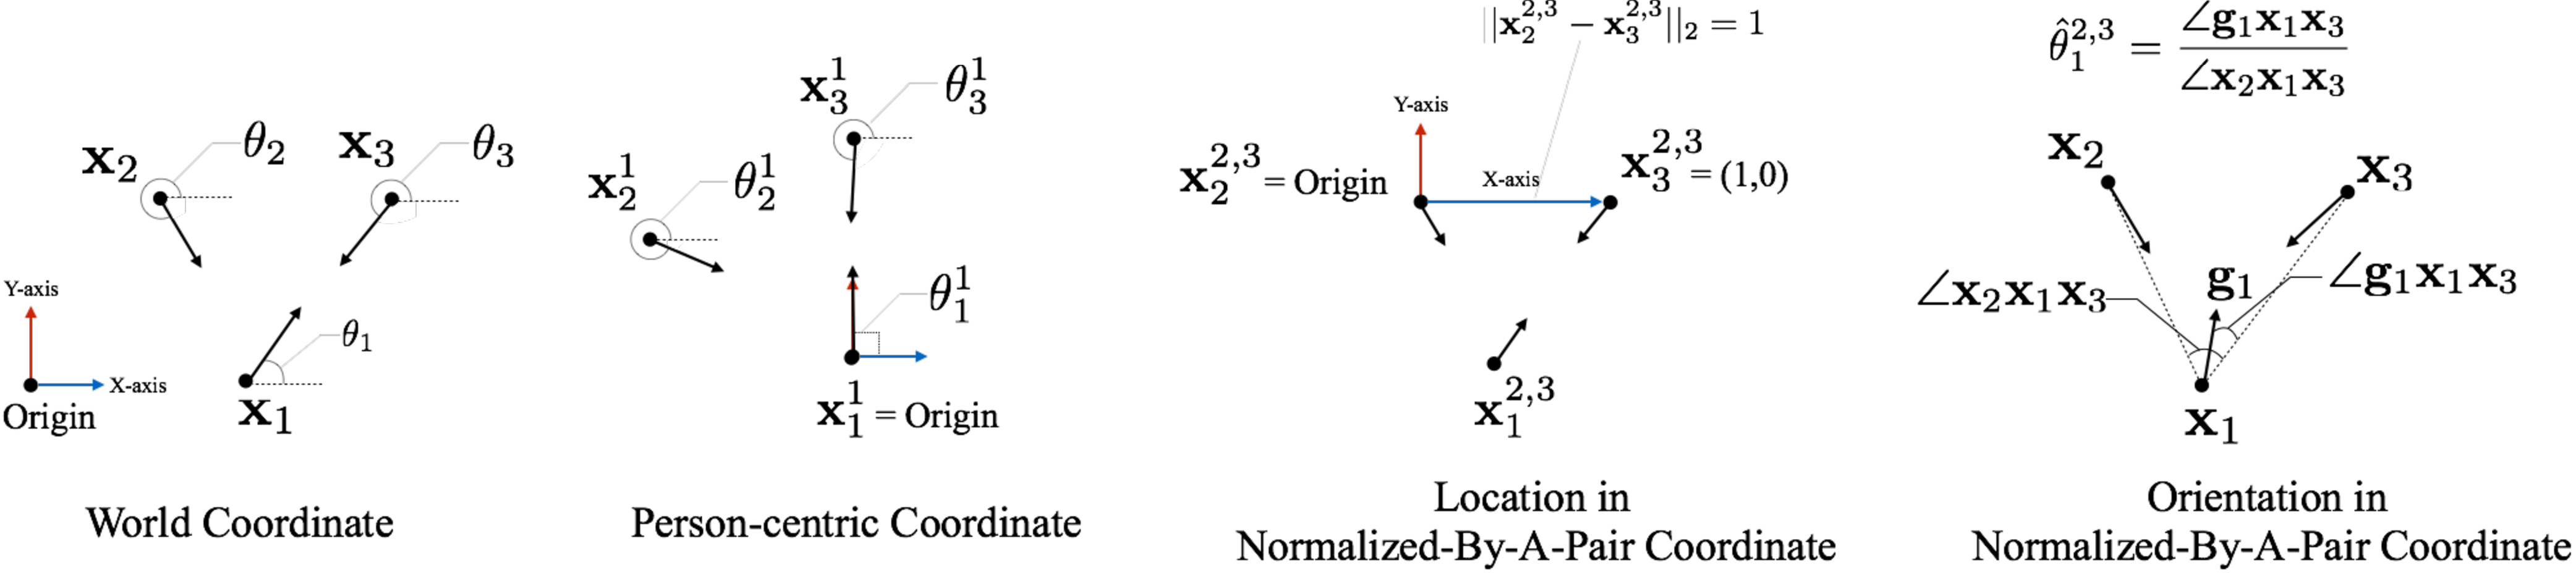
\includegraphics[width=\textwidth]{fig/ssp_notation3}
% 	\caption{Locations and orientations of an interacting group can be represented by different coordinate systems. (a) Locations and orientations in a world coordinate, (b) Locations and orientations in a person centric coordinate by person $\mathbf{P}_1$, (c) A location of $\mathbf{P}_1$  in a normalized coordinate by a pair of people $\mathbf{P}_2$ and $\mathbf{P}_3$, (d) An orientation of $\mathbf{P}_1$ in a normalized coordinate by a pair of people  $\mathbf{P}_2$ and $\mathbf{P}_3$. } 
% 	\label{fig:ssp_notation1}
% \end{figure*}

\subsection{Predicting Speaking}
\label{subsection:ssp_pred_speak}
As the first task, we predict whether the target subject is currently speaking or not, that is $\mathbf{S}^0$.  This is a binary classification task and relatively easier to train. We first study the correlation between the speaking signal and the target person's own social signals, either body motion or facial motion, or both. We expect this correlation is stronger than the link between individuals. We then compare it with the performance of a classifier that uses the conversational partner's social signals. More specifically, a function $\mathcal{F}_{J0\rightarrow S0}$ uses the target person's own body motion $\mathbf{J}^0(t_0:t)$ to predict the speaking signal:
\begin{gather}	
\mathbf{S}^0(t_0:t) = \mathcal{F}_{J0\rightarrow S0} \left( \mathbf{J}^0(t_0:t) \right),
\label{eq:speaking_0}
\end{gather}
and similarly,
\begin{gather}	
\mathbf{S}^0(t_0:t) = \mathcal{F}_{F0\rightarrow S0} \left( \mathbf{F}^0(t_0:t) \right),\\
\mathbf{S}^0(t_0:t) = \mathcal{F}_{(F0, J0)\rightarrow S0} \left( \mathbf{F}^0(t_0:t) , \mathbf{J}^0(t_0:t)\right),
\label{eq:speaking_0_facebody}
\end{gather}
where $\mathcal{F}_{F0\rightarrow S0}$ uses the target person's own face motion, and $\mathcal{F}_{(F0, J0)\rightarrow S0}$ uses both. 

We compare the performance of these functions with the functions that takes the signals from a communication partner, the other seller:
\begin{gather}	
\mathbf{S}^0(t_0:t) = \mathcal{F}_{J2\rightarrow S0} \left( \mathbf{J}^2(t_0:t) \right),\\
\mathbf{S}^0(t_0:t) = \mathcal{F}_{F2\rightarrow S0} \left( \mathbf{F}^2(t_0:t) \right),\\
\mathbf{S}^0(t_0:t) = \mathcal{F}_{(F2, J2)\rightarrow S0} \left( \mathbf{F}^2(t_0:t), \mathbf{J}^2(t_0:t) \right),
\label{eq:speaking_1}
\end{gather}
where the functions use body cues, face cues, and both cues, respectively. 

Equipped with this framework, we can computationally study the correlation of different types of social signals from the same individual and across individuals. We hypothesize that the correlations of the target person's own signals are stronger than the correlations among the interpersonal signals, while we still expect that there exists a clear link in the latter case. We verify this in our experimental results.

%the social signals oindividual dynamics of the social signals is stronger than correlation between the speaking and the social signal body motion should be stronger than the speaking of the target and other people's body motions. But we still presume that there exists a clear correlation in building the function ~\ref{eq:speaking_1}; for example, if another person is talking we can guess the target person is not speaking due the ``turn-taking" implicitly followed during a social conversation. % This study is interesting because it demonstrates the existence of social correlation among social signals.

\paragraph{Implementation Details.}
We use four 1-D convolutional layers (the first three networks have 128, 256, and 512 dimensional output features respectively and filter widths are 7 for all of them) for the network where the last layer has $1\times1$ convolutions, followed by a sigmoid activation layer. Our model does not require a fixed window size for the input, but we separate input data into small clips with a fixed size (denoted by $f$) for the efficiency in training. During testing time, our models can be applied to the input of arbitrary length. We use $f=120$, about 4 seconds, for the input window size. The feature dimension of the input of our network is the same as the concatenation of face motion and body motion (78 dimensions), but if fewer cues are used (e.g., face only or body only) we mask out the unused channels by keeping the same network structure for the fair comparison. We use the stochastic gradient descent algorithm Adam~\cite{kingma2014adam}. Dropout is also applied with a retention probability of 0.25.  

%The basic architecture follows the work of Holden et al.~\cite{holden2016deep} that demonstrates a compelling result for the mapping between a 2D trajectory and human motions. We modify the network architecture based on the input and output dimensions. 

%The network architecture is shown in the first row of Figure~\ref{fig:architectures}.
%\label{section:body2speak}
%The input of this network is the body motion of the other seller in the haggling sequence, which is a $f \times 73$ matrix, where $f$ is the number of frames of an input sequence. Here, we ignore the buyer's body motion because often little movement is observed from the buyers.  

\subsection{Predicting Social Formations}
We predict the location and orientations of the target person. This problem is strongly related to Proxemics~\cite{Hall66} and F-formation~\cite{kendon90}, illustrating how humans use their space in social communications.
\begin{gather}	
 \mathbf{Y}_p (t_0:t) = \mathcal{F}_p \left( \mathbf{X}_p^1(t_0:t), \mathbf{X}_p^2(t_0:t) \right),
 \label{eq:pred_formation}
\end{gather}
where $\mathbf{Y}_p$ and $\mathbf{X}_p^i$ contains global location and orientation signals $[\mathbf{x}, \boldsymbol{\theta}, \boldsymbol{\phi} ]$ for the target subject and others.
Note that we only consider the positions and orientations on the ground plane (in 2D), ignoring the height of the subjects. Thus $\mathbf{x} \in \mathbb{R}^2 $ representing $x$ and $z$ coordinate of the subjects. We use a 2D unit vector to represent the orientations $\theta \in \mathbb {R}^2$ and face orientation $\phi \in \mathbb{R}^2$, because the angle representation has a discontinuity issue when wrapping around $2\phi$ and $-2\phi$. In summary, $\mathbf{X}^i(t)$ and $\mathbf{X}^i(t)$ are a $6 \times N$ dimensional matrix where $N = t- t_0$ is the size of the temporal window. This prediction problem is intended to see whether the machine can learn how to build a social formation to interact with humans~\cite{vazquez2017towards}. %We Social formation is one of the most noticeable social properties with strong correlation, allowing us to easily evaluate the performance.


\paragraph{Implementation Details.}
We use a 2D vector for the position and 2D unit vectors for the face orientation and body orientation, defined on the $xz$-plane. Thus the status of an individual at a frame in social formation prediction is represented by a 6-dimensional vector.


The input of the social formation network is the concatenation of global position and orientation information of the communication partners, represented by a $f \times 12$ matrix.  We use a simple autoencoder structure, as shown in the second row of Figure~\ref{fig:architectures}.


%To implement this, we use a simple 1-D temporal convolutional neural network to model $\mathcal{F}_p$. The network is trained with a window of frames $N=120$ (corresponding to 4 seconds), but arbitrary length of input can be used in testing time since our network is fully convolutional. We use a simple encoder-decoder network. The encoder has  3 convolutional layers followed by dropout (0.25) and RELU, and 1D pooling layer (with stride 2). The decoder uses a single transposed convolution layer. We use L2 loss function with a L1 regularization term (with weight 0.1). We simply use the global position and orientations with standardization, rather than any local or relative coordinate.

% !TEX root = ../thesis.tex

\section{Network Architectures}

In this section, we describe the implementation details of the neural network models we build for social signal prediction. Our method takes the social signals from conversational partners as input and produces the target person's social signals as output. Figure~\ref{fig:inputOutput} shows 3D measurements used for the input and output of our method, where the signals rendered by green and yellow colors are the input, and the social signals rendered by blue color are the output. The output signals include social formation information (position, face orientation, and body orientation), and body motion, and a binary label for the speaking status of the target person. 

In our method, we divide the social signal prediction task into several sub-tasks focusing on predicting a subset of social signals, and the corresponding network architecture for each task is shown in Figure~\ref{fig:architectures}. All of our networks are based on 1D fully convolutional neural networks. In general, our model does not require a fixed window size for the input, but we separate input data into small clips with a fixed size (denoted by $f$) for the efficiency in training. During testing time, our models can be applied to the input of arbitrary length. We use $f=120$, about 4 seconds, for the input window size. The basic architecture follows the work of Holden et al.~\cite{holden2016deep} that demonstrates a compelling result for the mapping between a 2D trajectory and human motions. We modify the network architecture based on the input and output dimensions. 

\subsection{Dimensions of Social Signal Representations}
We describe the dimensions of social signal representations, used for the input and output of our method.

\paragraph{Trajectory (Position + Orientations):} We use a 2D vector for the position and 2D unit vectors for the face orientation and body orientation, defined on the $xz$-plane. Thus the status of an individual at a frame in social formation prediction is represented by a 6-dimensional vector.

\paragraph{Body Gestures:} We follow the body motion representation of the work of Holden et al.~\cite{holden2016deep}, representing a body gesture at a frame as a 73-dimensional vector. This representation is based on the skeletal structure of CMU Mocap dataset~\cite{gross2001cmu} with 21 joints (63 dimensions), along with additional dimensions for a floor point (3 dimensions), velocities for the root movement (3 dimensions relative body translation and orientation), and footstep signals (4 dimensions). We perform a retargeting to convert our 3D motion data from the Panoptic Studio (following the skeleton definition of COCO dataset~\cite{coco-14}) to this CMU Mocap format. For the face signal we use a subpart (initial 5 dimensions) of the facial expression parameters of Adam model~\cite{joo2018,cao2014facewarehouse}, because we found the later dimensions have almost negligible in our reconstruction quality.

\begin{figure}[t]		
	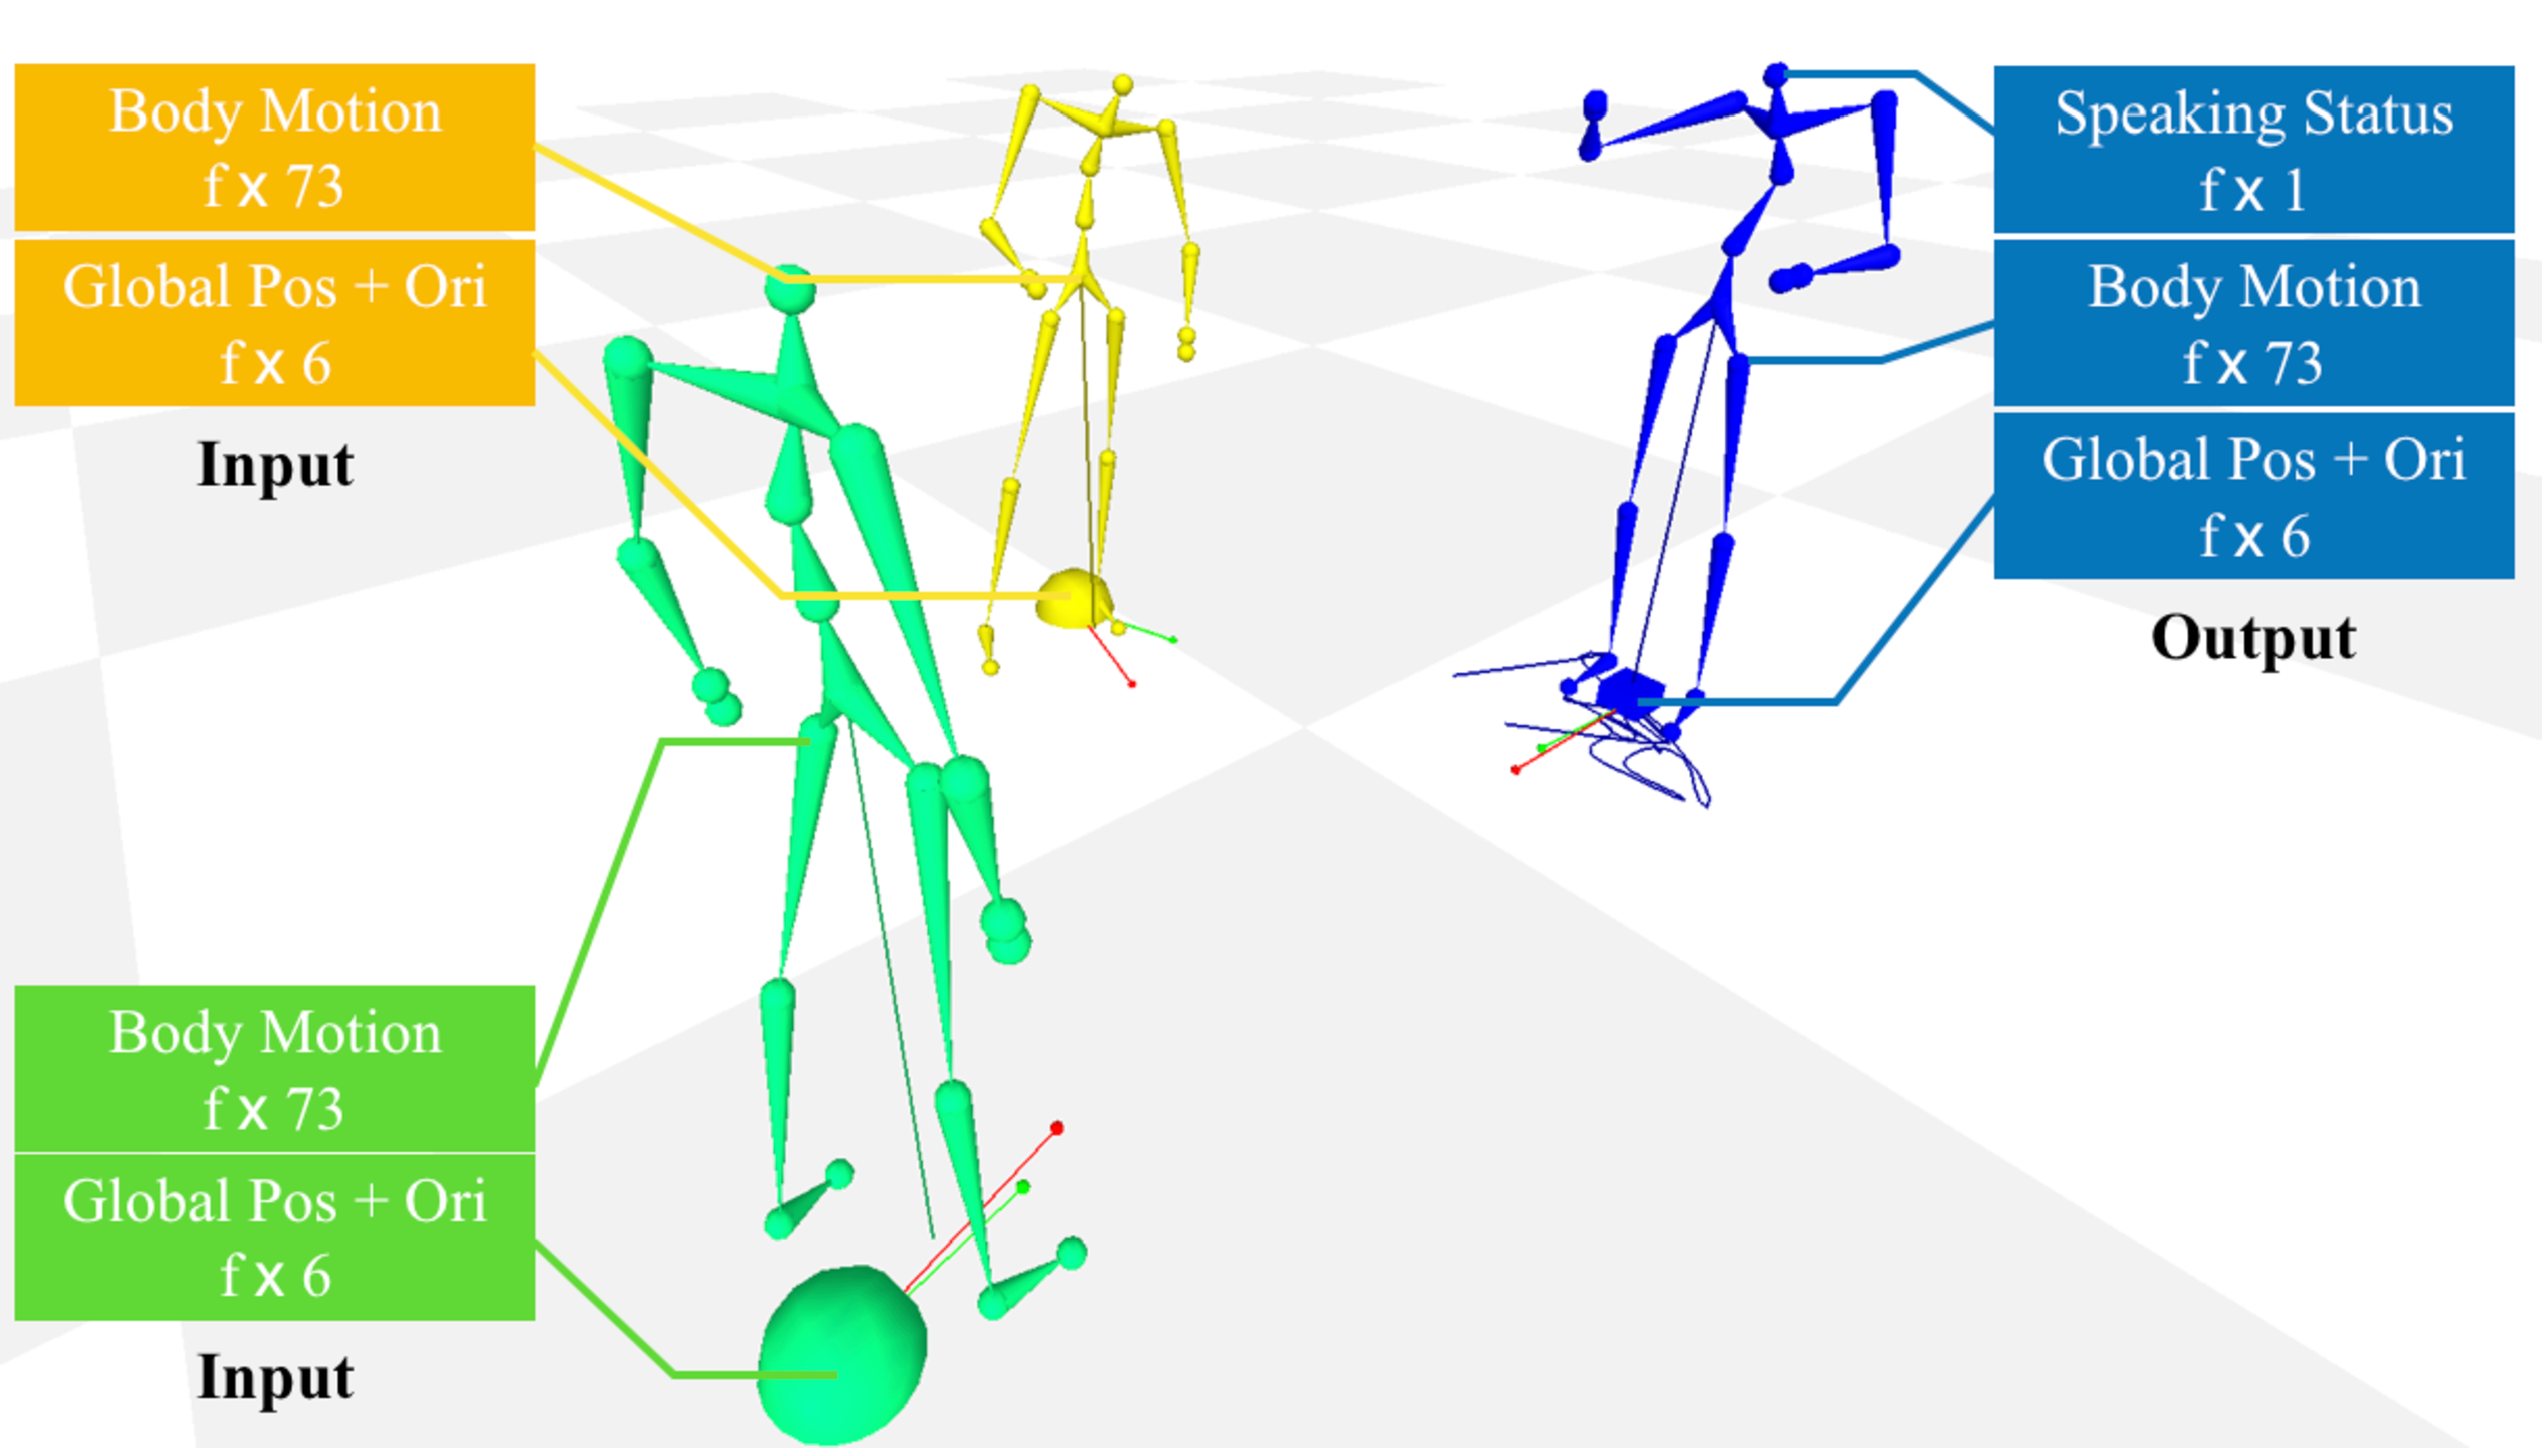
\includegraphics[width=\linewidth]{ssp_fig/Input_output.pdf}
	\caption{The input and output of the Social Signal Prediction task. Our method uses the social signals of conversation partners (green and yellow) as input, and produces the target person's social signals (blue) as output. We consider input and output with an arbitrary length, where the length is denoted as $f$ in this figure. The second dimensions of input and output matrices represent the dimensions of social signals in our representation.}
	\label{fig:inputOutput}
\end{figure}

\begin{figure*}[t]	
	%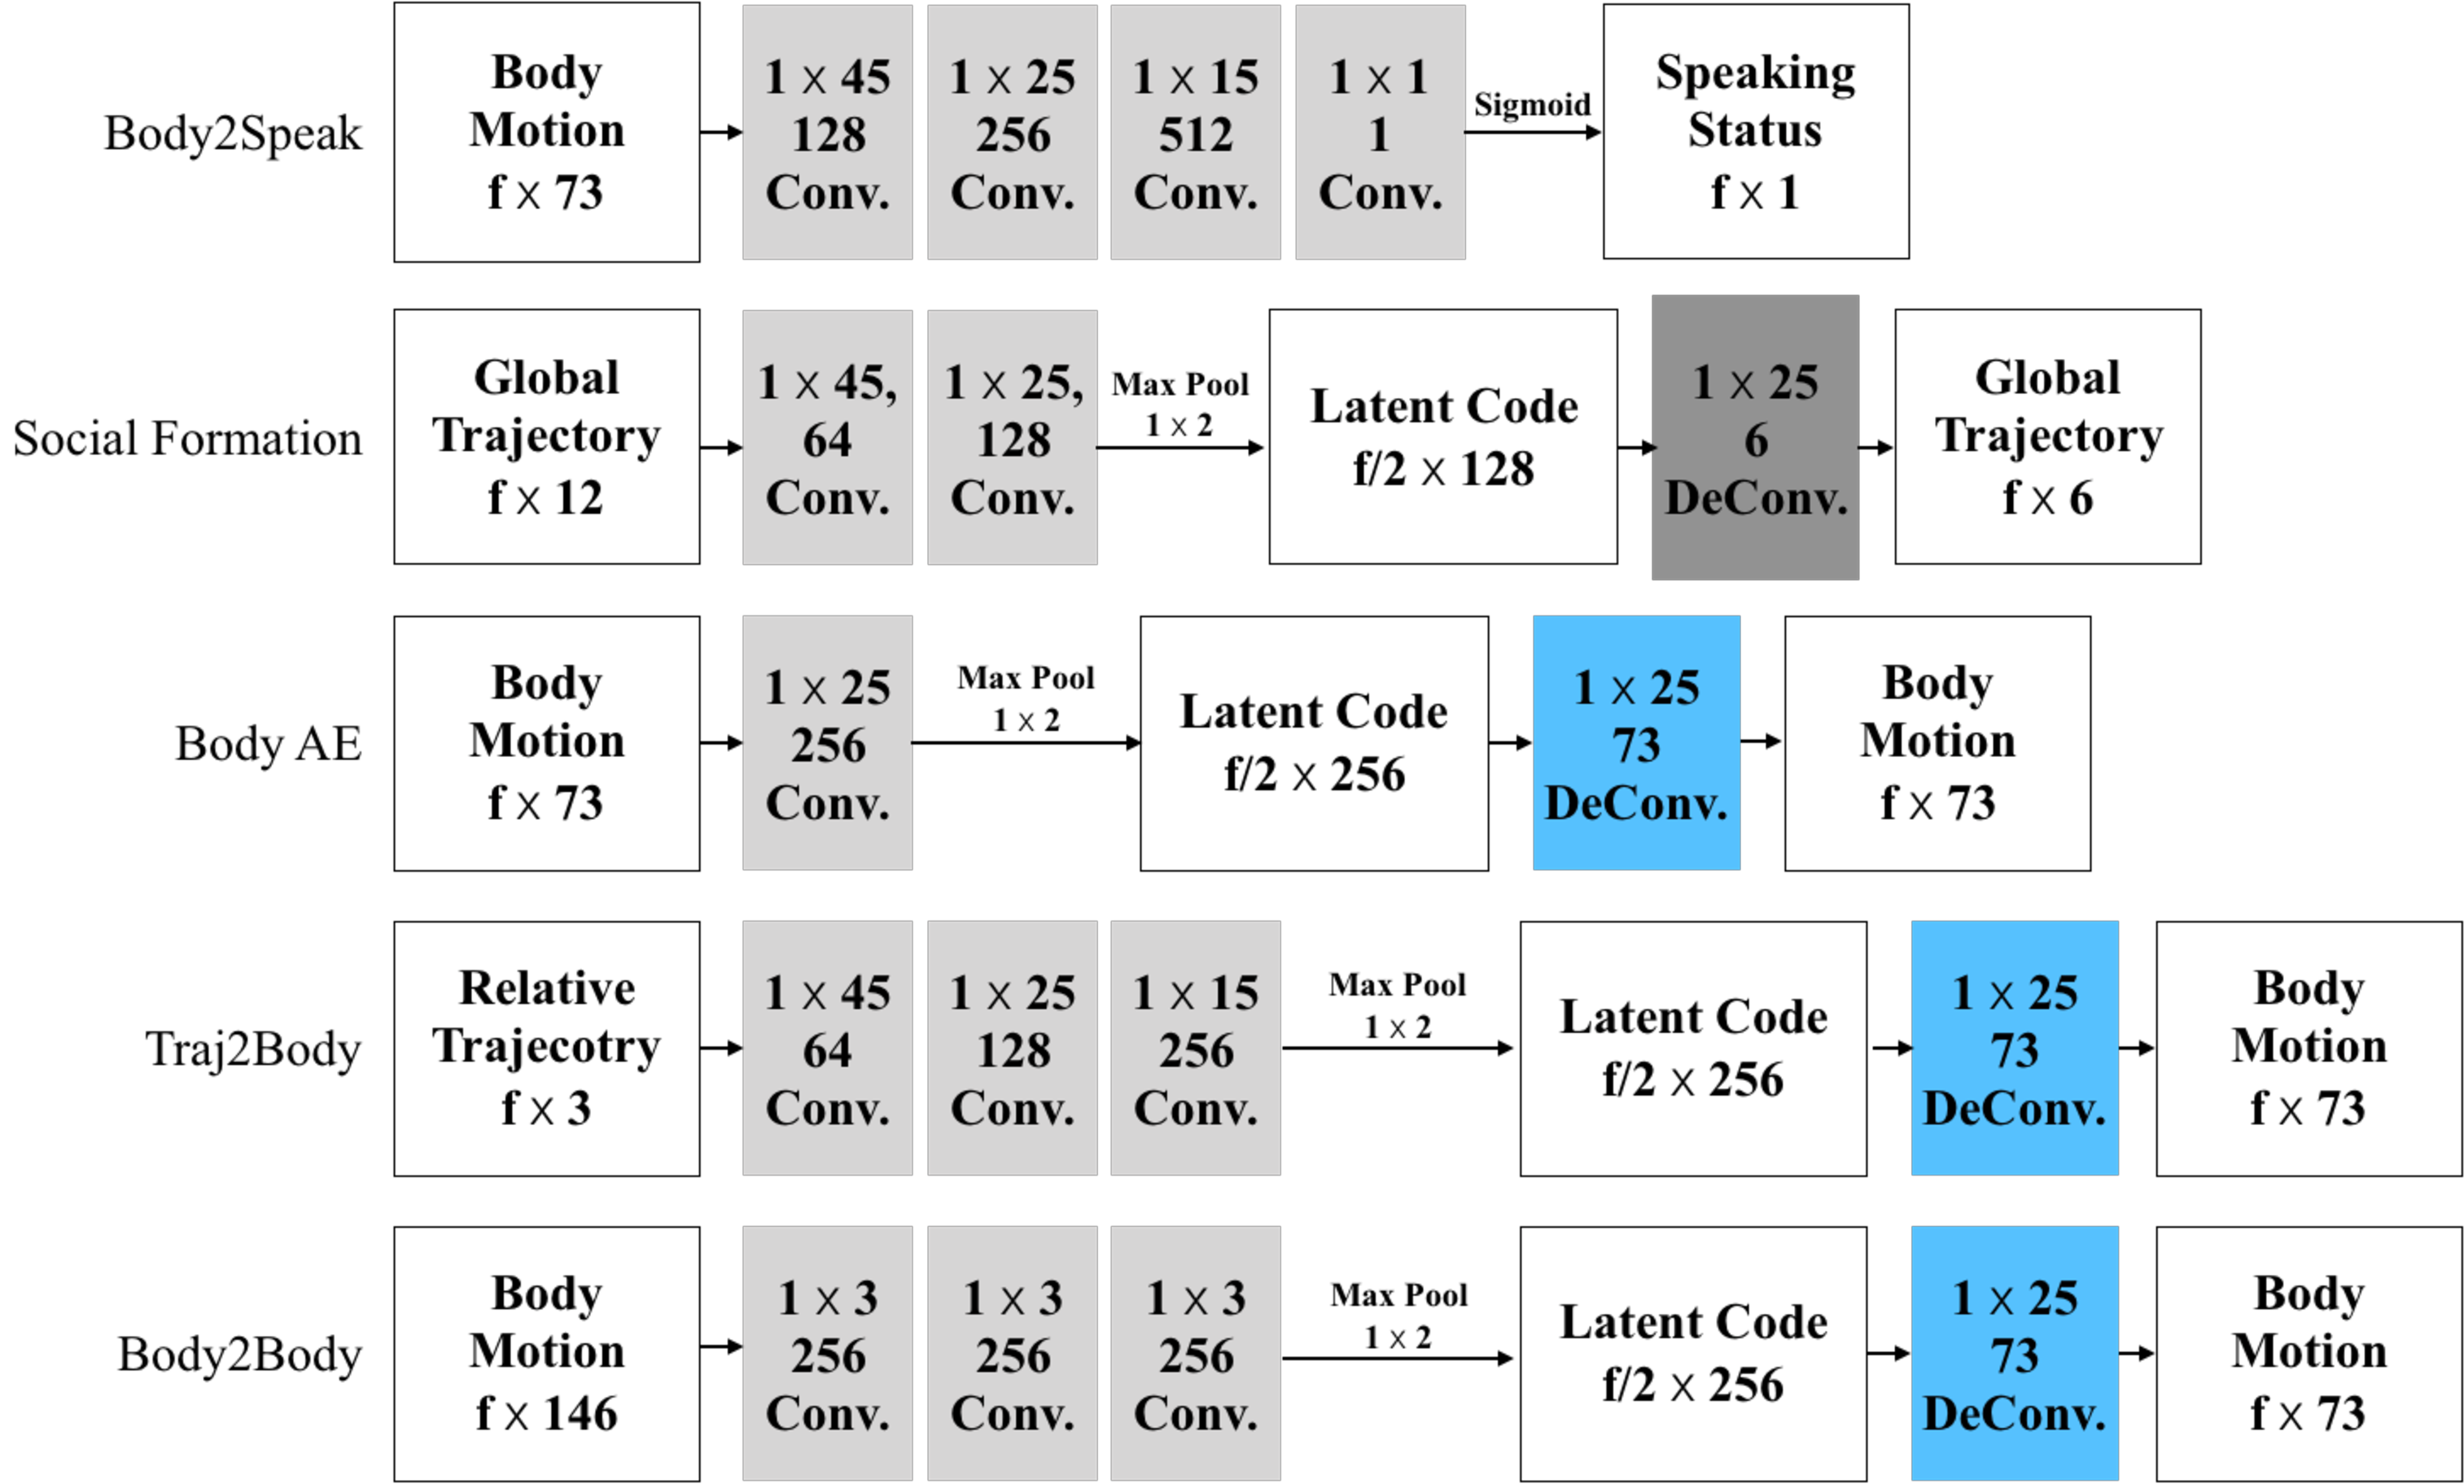
\includegraphics[width=\textwidth]{ssp_fig/networks}
	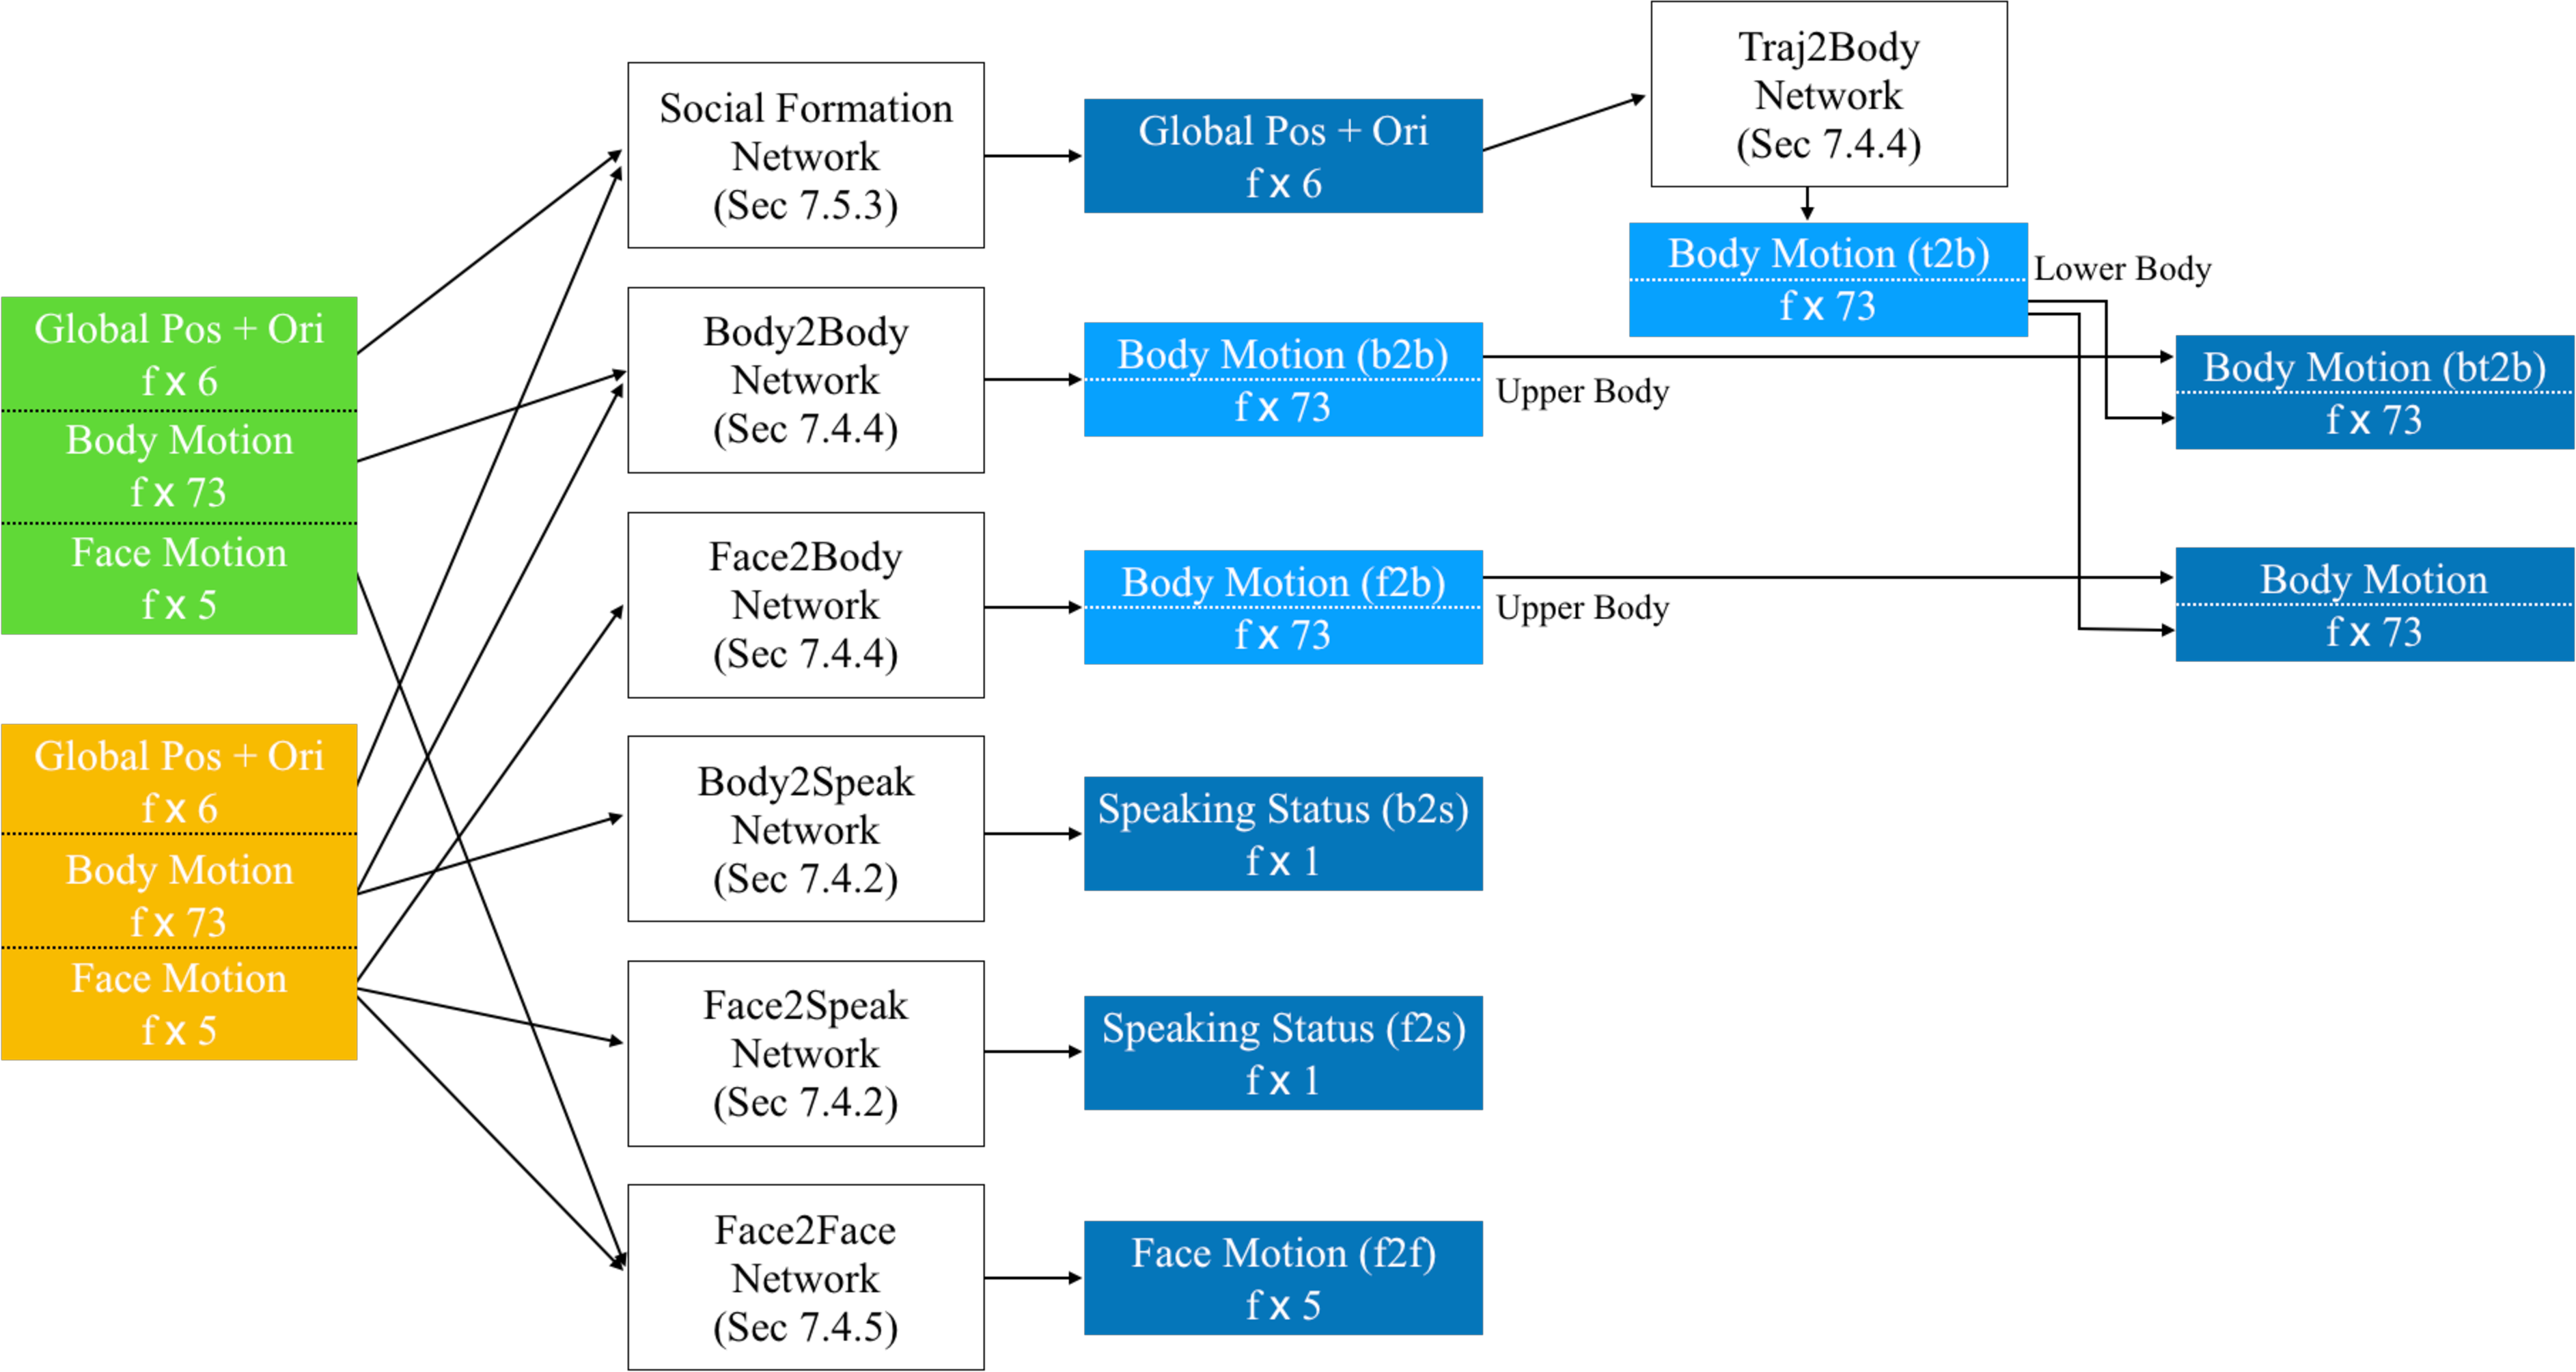
\includegraphics[width=\textwidth]{ssp_fig/networks_all}
	\caption{Network Architectures. We use fully convolutional networks to predict sub-parts of our social signal prediction. We adopts the architecture of Holden et al.~\cite{holden2016deep}, and modify the dimensions and structures based on the input and output dimensions. }
	\label{fig:architectures}
\end{figure*}



\subsection{Predicting Speaking from Body Motion (Body2Speak)}
The input of this network is the body motion of the other seller in the haggling sequence, which is a $f \times 73$ matrix, where $f$ is the number of frames of an input sequence. Here, we ignore the buyer's body motion because often little movement is observed from the buyers.  We use four convolutional layers for the network where the last layer has $1\times1$ convolutions, followed by a sigmoid activation layer. The network architecture is shown in the first row of Figure~\ref{fig:architectures}.


\subsection{Social Formation}
The input of the social formation network is the concatenation of global position and orientation information of the communication partners, represented by a $f \times 12$ matrix.  We use a simple autoencoder structure, as shown in the second row of Figure~\ref{fig:architectures}.

\begin{figure*}[t]	
%	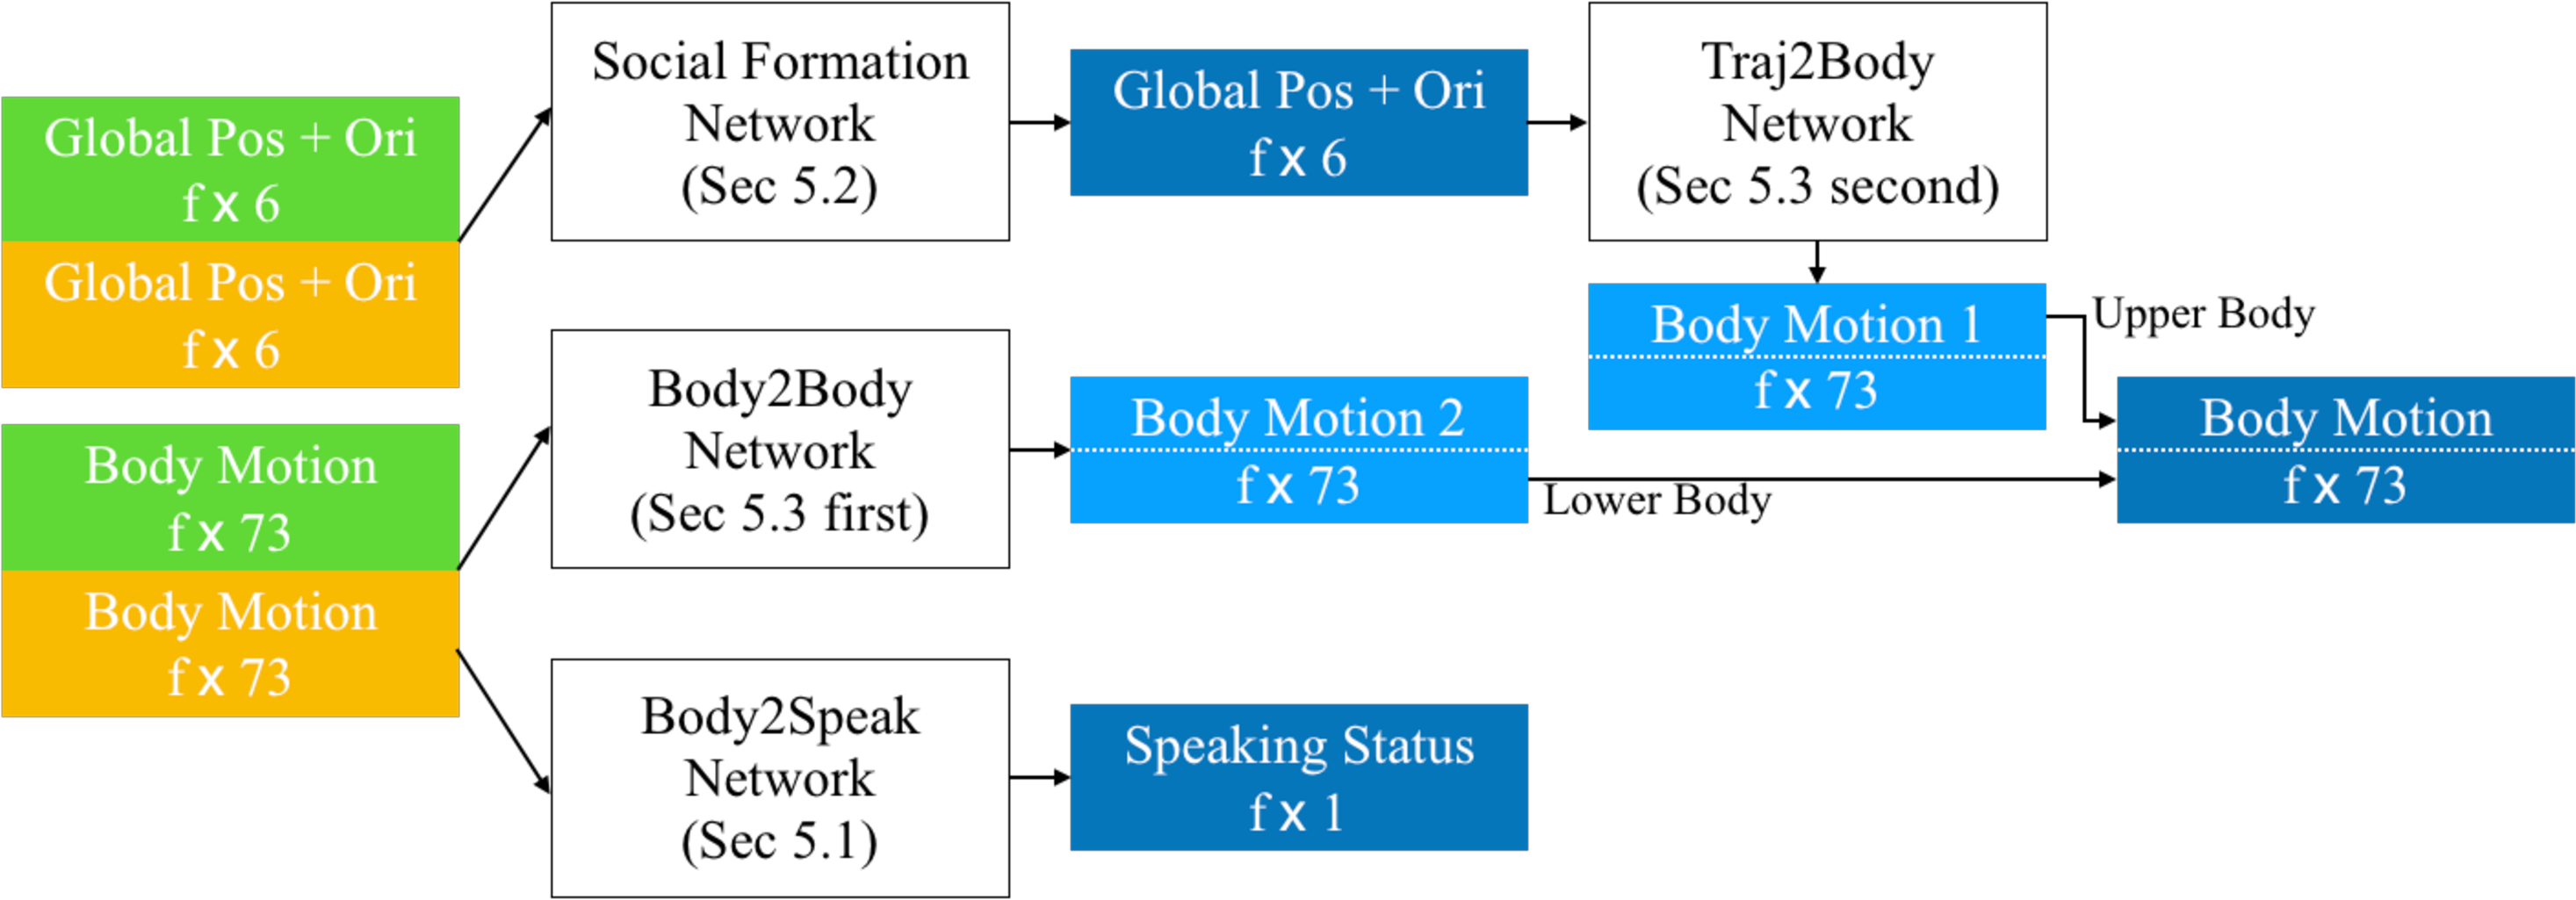
\includegraphics[width=\textwidth]{ssp_fig/ssp_pipeline}
	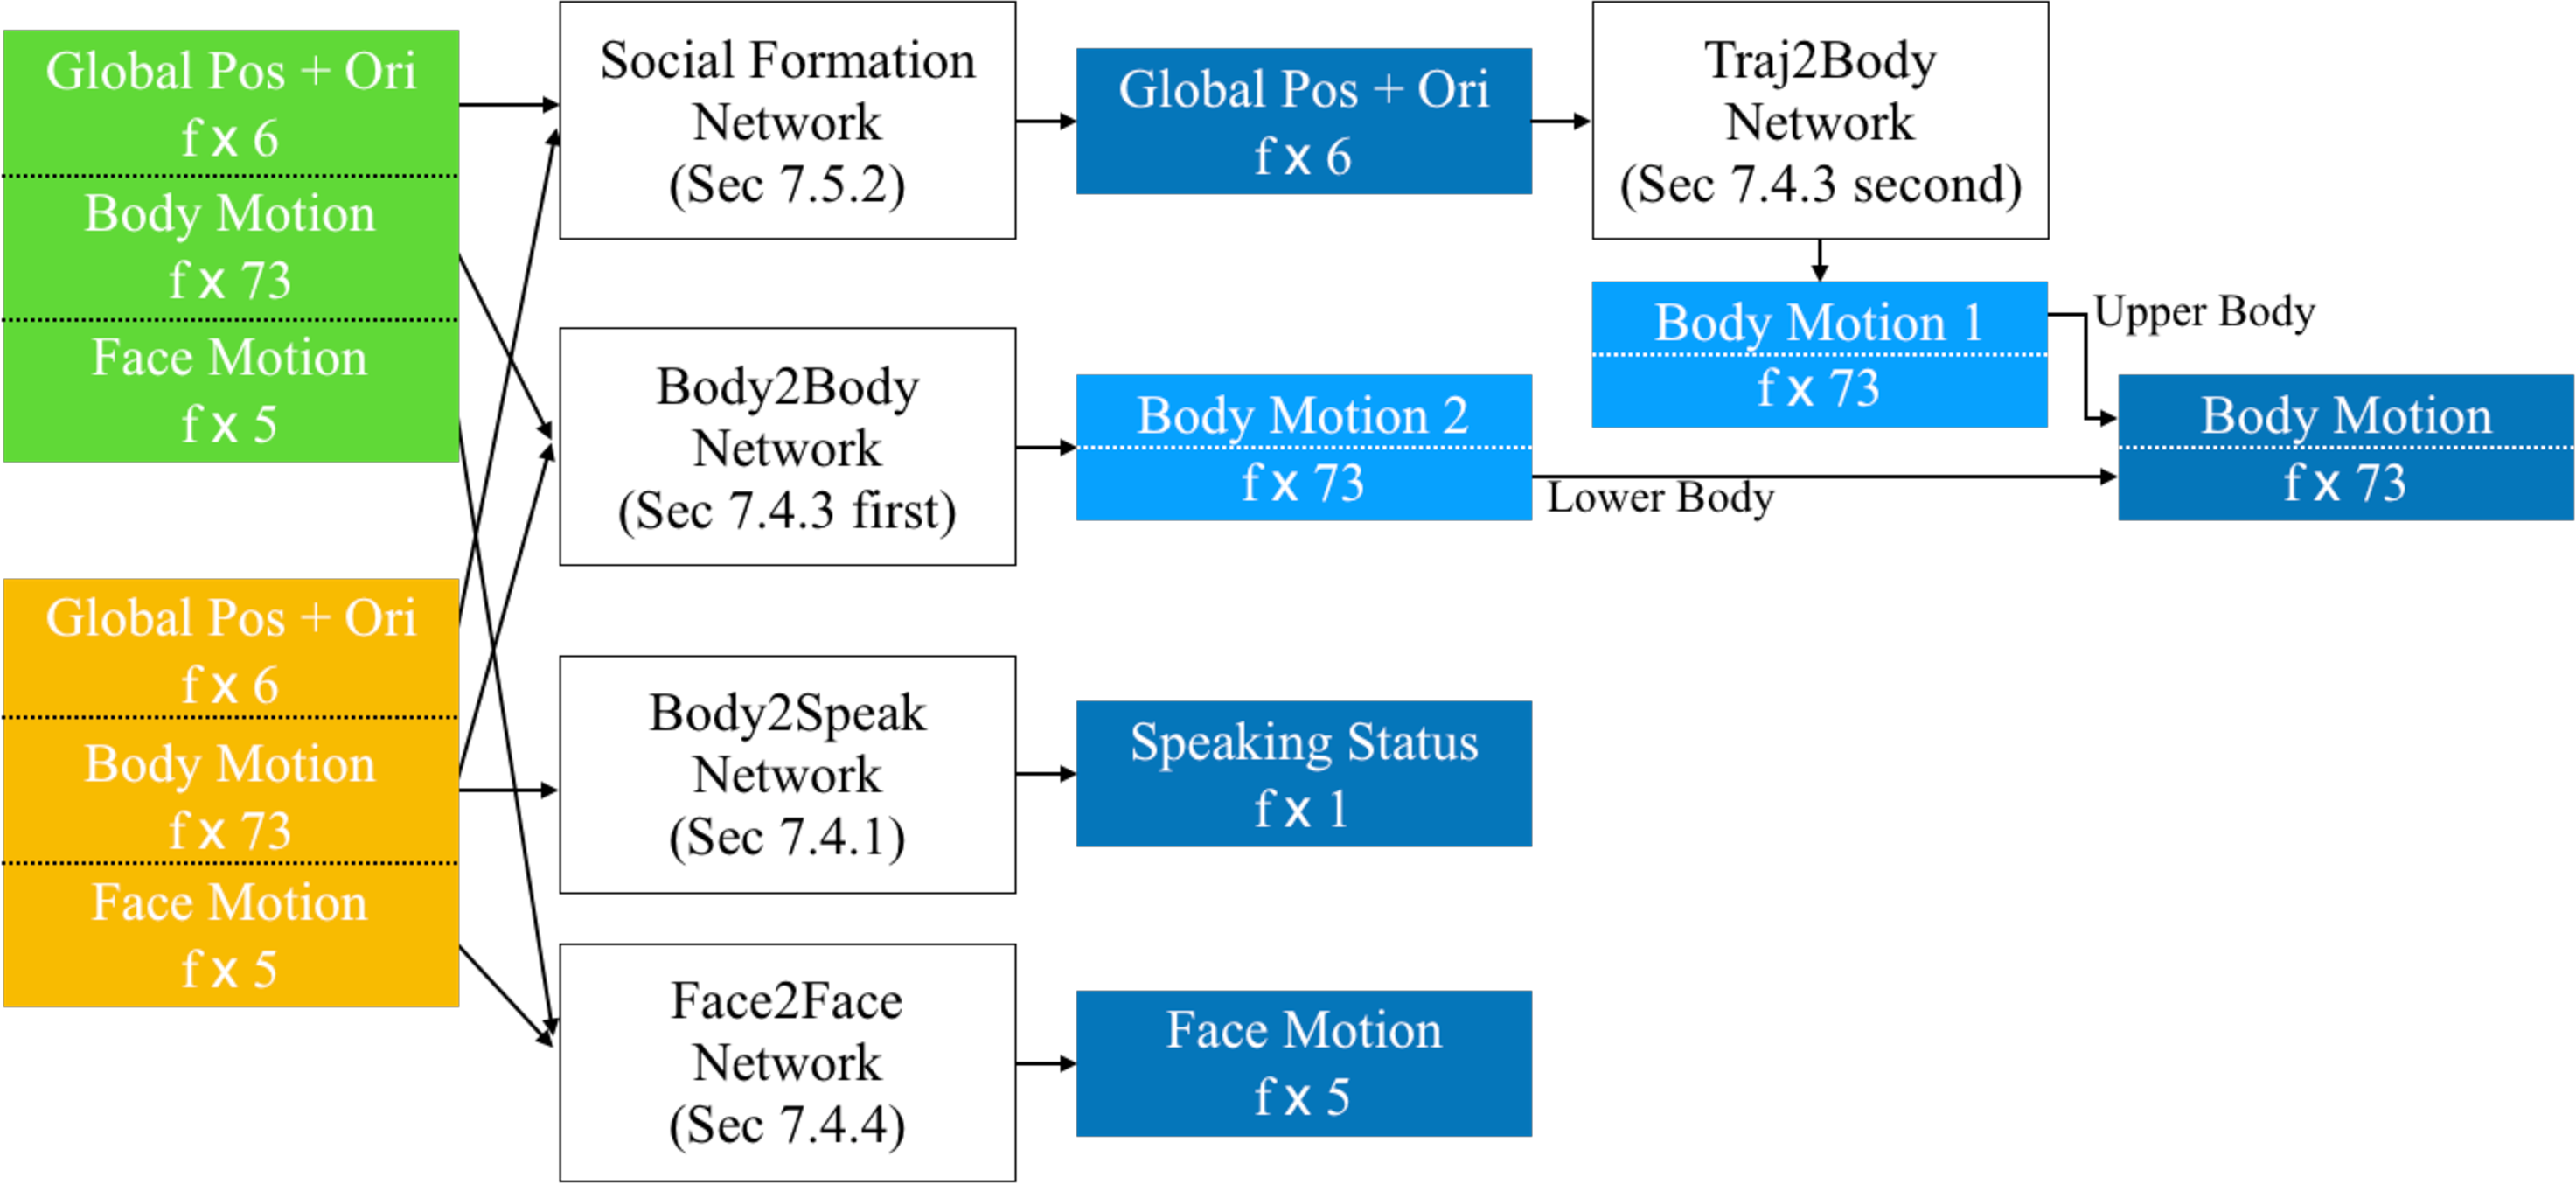
\includegraphics[width=\textwidth]{ssp_fig/ssp_pipeline_wFace}
	\caption{Our Social Signal Prediction Pipeline. We present a baseline method to predict position, orientations, and body gestures, and speaking status of the target subject. }
	\label{fig:pipeline}
\end{figure*}

\subsection{Autoencoder to learn body motion manifold}
\label{sec:autoencoder}
As a preprocessing for body gesture prediction tasks, we first learn the manifold space of the body motion, following the work of \cite{holden2016deep}. We found that this approach is essential to restrict the motion prediction output in a feasible human motion space. We use the same network architecture with \cite{holden2016deep}, using a single convolution layer for each encoder and decoder. The network is shown in the third row of  Figure~\ref{fig:architectures}. The dimension of the latent space is 256 with the half window size of the input, which is larger than the original dimension. Similar to the work of ~\cite{holden2016deep} we add an L1 regularizer in the loss function. After the training, we freeze the decoder part, and use it to decode body motion from the latent code predicted by social prediction tasks.

\subsection{Predicting Body Gestures From A Trajectory (Traj2Body)}
\label{sec:traj2body}
As a baseline method, we regress body motion from the estimated trajectory information of the target person (position and body orientation), as described in Equation~\ref{eq:pred_p2J}. As input, we use the velocities of position and body orientation (relative root movements with respect to the previous frame), which is a part of our body motion representation. For training, we use the ground truth body motion data, where the subpart representing relative root movements as input, and all dimensions of body motion as output. During the testing, we convert the social formation prediction output (global position and orientation) into this velocity representation (relative position and orientation), and use it as the input for our prediction network. The network architecture is shown in the fourth row of Figure~\ref{fig:architectures}. The network predicts the latent code in the body motion manifold space from the 2D trajectory input, and final motion is generated by using a freeze decoder from subsection~\ref{sec:autoencoder}. Note that the decoder is fixed in both training and testing. 

\subsection{Predicting Body Gestures from Other Body Gestures (Body2Body)}

In this case, we use the other two partners' body motions as input. Different from the ``Traj2Body" network in the subsection \ref{sec:traj2body}, we use smaller filter sizes, because we empirically found it makes the body motions more diverse. The network is shown in the fifth row of Figure~\ref{fig:architectures}.

\subsection{Predicting Face Signals from Other Face Signals (Face2Face)}

We use a similar framework with body gesture prediction by learning a manifold space via an autoencoder and predicting the latent code using a regressor, as shown in the sixth row of Figure~\ref{fig:architectures}.

\section{Pipeline of Our Social Signal method}
Each subtask focuses on predicting a part of social signals of the target subject.  To this end,  the predicted social signals are consolidated together to mimic the target person's social behaviors, responding to behaviors of conversational partners. The figure~\ref{fig:pipeline} shows the illustration of the pipeline, where the dark blue boxes are the final outputs. 

% !TEX root = thesis.tex

\section{Evaluating Social Signal Prediction}
\label{section:evaluation}
The output of social signal prediction should satisfy two core requirements: (1) The predicted signals should be within a feasible human motion space showing realistic human motions (realistic motion requirement), and (2) The predicted signals should follow the social rules, spatially and temporally responding to the behaviors of communication partners (social motion requirement). However, it is challenging to qualitatively evaluate these requirement, because there is no objective metric to measure ``realistic" or ``social" behaviors. %The ``realistic motion" requirement can be considered as a necessary condition for the ``social motion" requirement, because non-realistic motion is not acceptable and cannot be suitable to social situations. But it is not sufficient, because realistic jogging motion, satisfying the first condition

Notably, the L2 distance between the predicted signals and ground-truth may not be a good metric because it does not assume diverse possible solutions. Given the same input, human behavior can be still acceptable, but these are penalized if it is different from the ground-truth motion. Due to the reason, L2 metric favors the mean of the data distribution, although it is qualitatively far from expected output. Similar issues have been discussed in human motion forecasting area~\cite{mnih2012conditional, Fragkiadaki_2015_ICCV, jain2016structural}, since there can be diverse possible human motions given a history of input motion. Due to the issue, the area mainly focuses on short-term forecasting (at most several seconds).


In this work, we present a new approach to better evaluate social signal prediction results. We found that for some subpart the L2 distance is reliable, showing that a lower error means a better quality. Classifying speaking status is an example of it. However, if the dimension of the output signals is high, such as body motion, the L2 metric does not consistent to the actual quality of the output. Our idea is evaluating the social signal prediction output by transferring it into easier signal space. As an example, we use our model that regresses speaking status given body motion, and the quality of the body motion is evaluated by computing the accuracy of the speaking status. Speaking signal in our social scenario is an important social cue, which is mainly related to the turn taking rule of communication, and this metric only penalizes such properties. Although this metric is not ideal due to the imperfection of our speaking status regressor, we found that this metric provide a consistency to the qualitative performance of the output. The pipeline of this metric is shown in Figure~\ref{fig:evaluation_bySpeakclass}.


%Good metric is also closely related in training a better model, because the metric can be directly used as a loss function in learning stage. for loss function in the neural network architecture. This is one of the biggest challenging in evaluating the performance of the social signal prediction, and it also related to the loss function in training our models.





%penalize the realist signals if it is deviated from the ground-truth. As an example, in our in synthesizing body gestures, a mean of the entire pose distribution shows very competitive L2 errors compared to predicted output, although qualitatively the mean pose does not satisfy either requirements. Similar issues have been discuss in the forecasting single person's human motions~\cite{mnih2012conditional, Fragkiadaki_2015_ICCV, jain2016structural}. It should be noted that the same metric is also used in training models (e.g., neural network), which makes the output of the model converges to the mean pose in the end. 




%The work in forecasting motion of a single subject focuses on the first requirement~\cite{mnih2012conditional, Fragkiadaki_2015_ICCV, jain2016structural}, and the area suffers from the deficiency of a good evaluation method. The L2 distance between the predicted signals and ground-truth motion is often used


% while the second requirement is more challenging and rarely demonstrated. For example, any arbitrary ground-truth motion capture data can satisfy the first condition (because they are genuine signals of humans), and arbitrary combinations of such motions with smooth transition still can satisfy the condition~\cite{kovar2008motion}, but the second condition can be achieved by properly modeling social communication.
%
%Both requirements are hard to be evaluated.
%
%Good metric is also closely related to learining better model, because the metric can be directly used for loss function in the neural network architecture. This is one of the biggest challenging in evaluating the performance of the social signal prediction, and it also related to the loss function in training our models.
%
%
%We found for some subpart of signals, this L2 metric provided consistent output as in qualitative evaluation, for example, in speaking classification and social formation estimation. They are hard to be applied for more high dimensional signal such as body signal. 
%
%
%
%We can use a human manifold space to evalute the first requirement. If output is far from this manifold space, then we can consider they are less realistic motion; that is the distance between the projected point to the original signal would be an evaluation metric. However, this requires a well-defined manifold space, which is a challenging issue. Moreover, since our motion output are synthesized by this manifold model, they tend to located in the space already, providing biases in evaluation. This output is discussed in Section~\ref{chapter:manifold_metric}. 
%
%The second requirement is very challenging without objective way to measure, due to the inherent diversity of human behaviors. Given an input signals of others, there could be several possible reaction of humans, which all can be possible solution, if it is within our social norms. A common evaluation metric, L2 distance, may penalize the realistic motion if it is far from the ground truth motion measured in our system. 
%
%We present an indirect method as a way to quantitatively measure the quality of prediction output. We use our trained network which takes body motions and produces signals which can be more reliably evaluated (e.g., speaking signals). Since the timing of speaking is closely related to the social interaction (turn taking), it can be used to evaluate the social requirement. We found that this method shows a reasonable output by penalizing the mean pose and favor the qualitatively better estimation output. This output is discussed in Section~\ref{chapter:classifier_metric}. 



\begin{figure}
	\centering       
	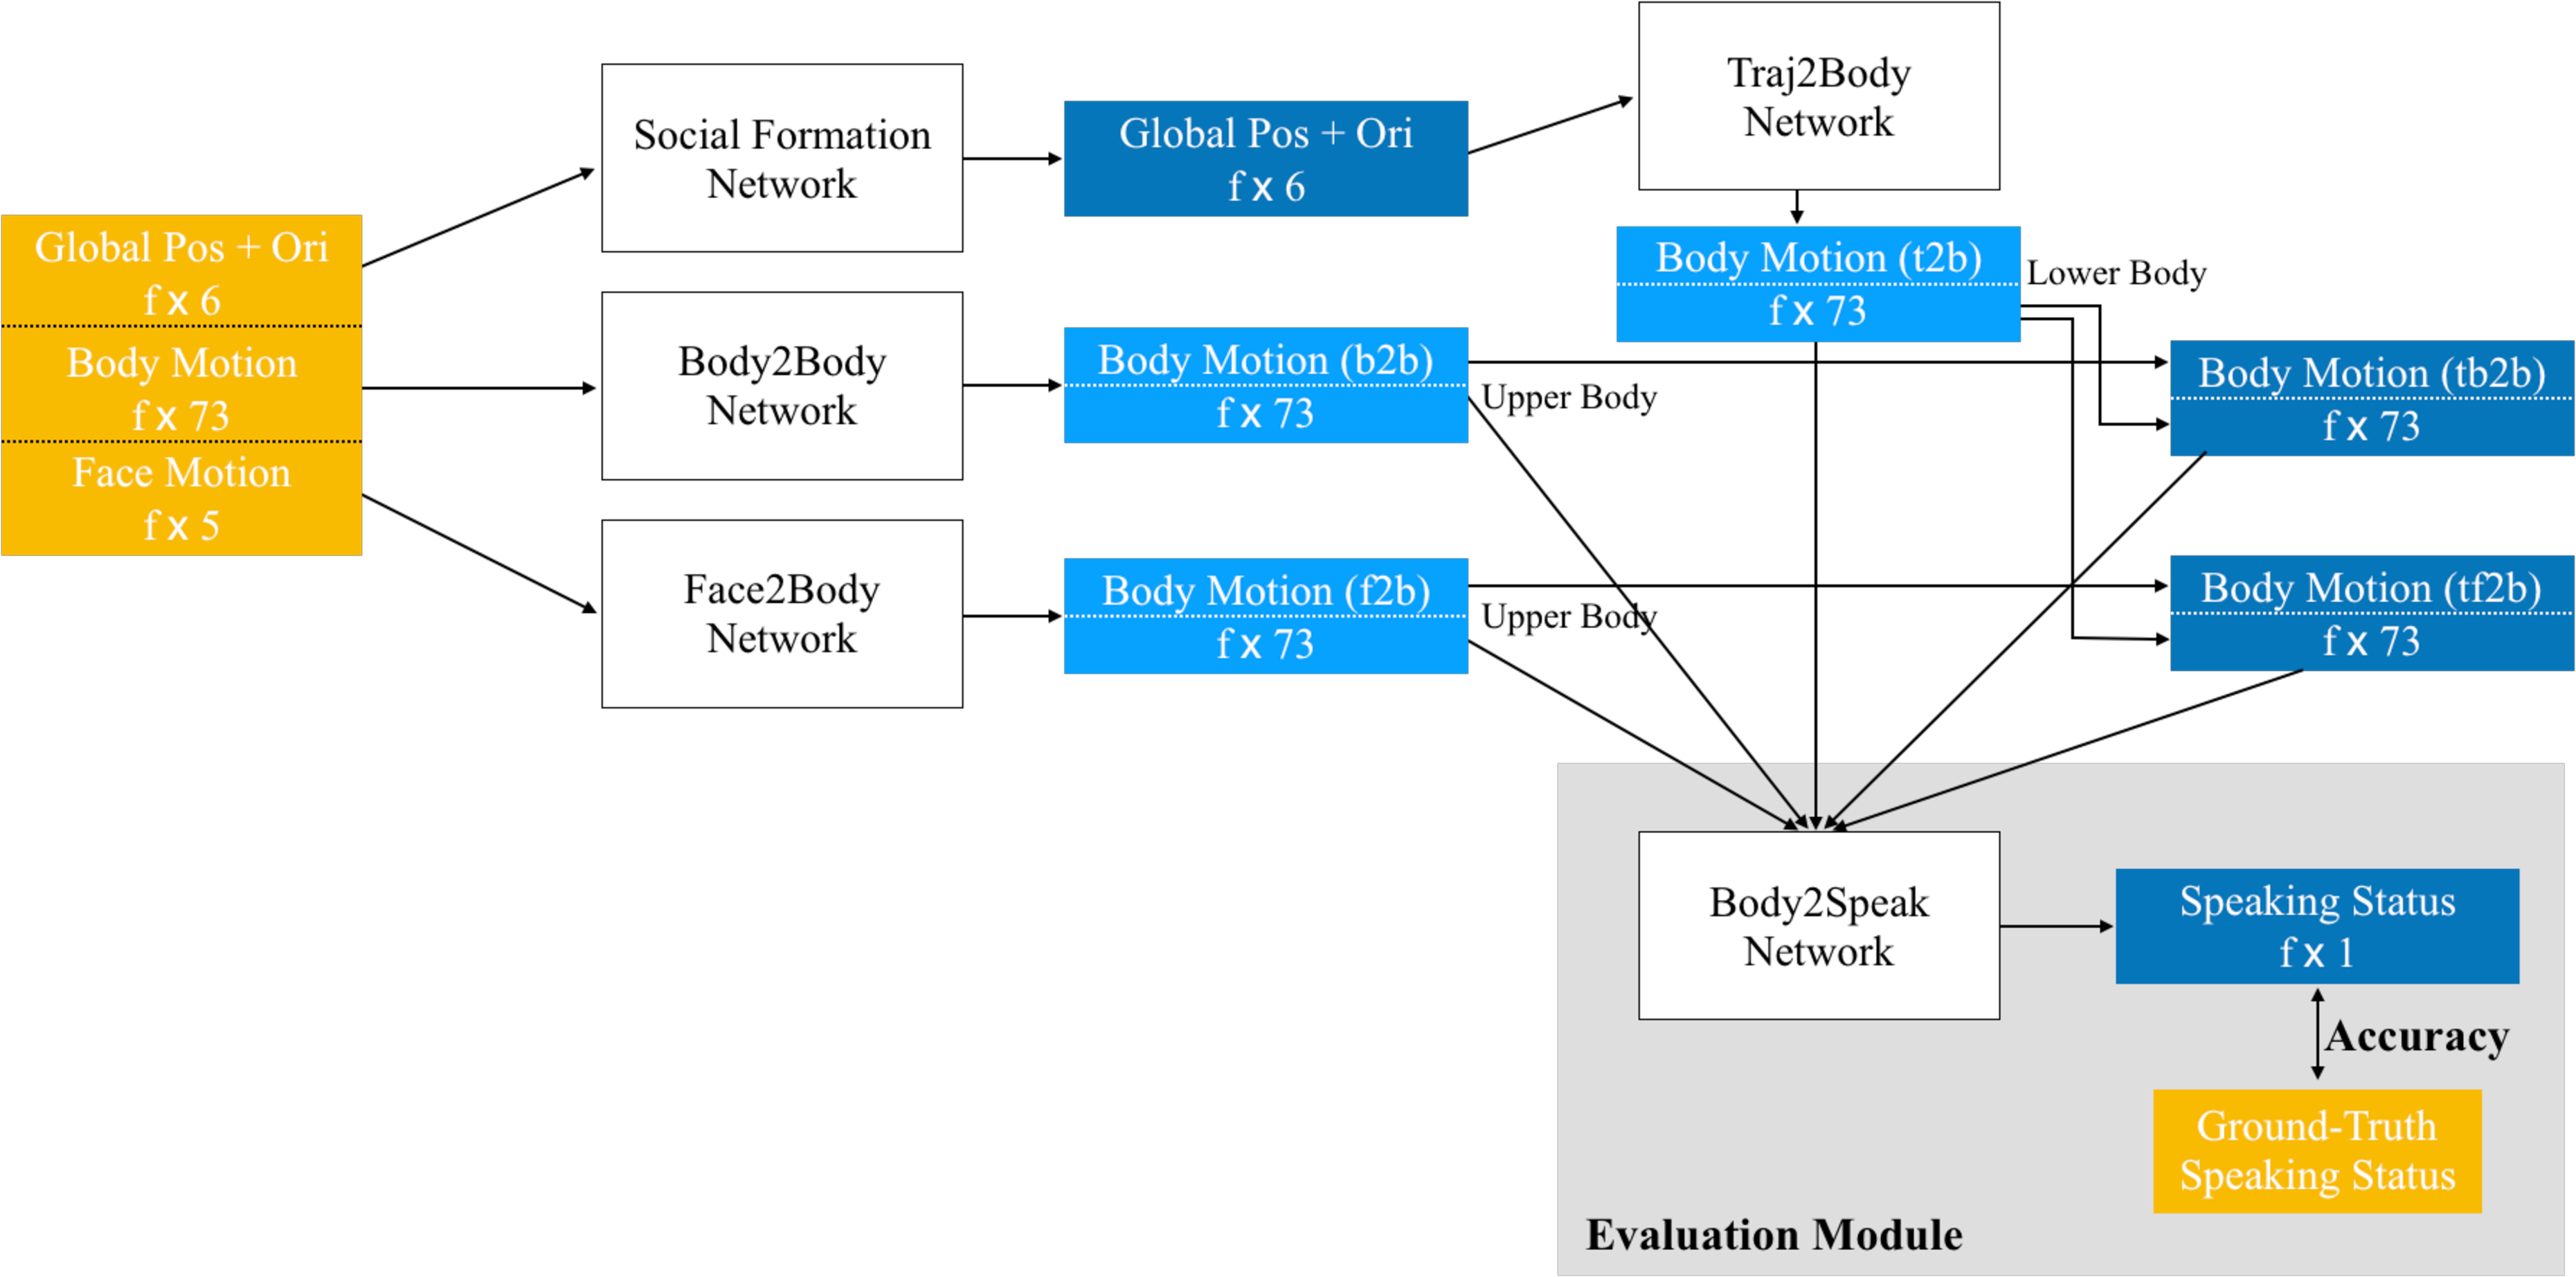
\includegraphics[ width=0.8\linewidth]{ssp_fig/evaluation_pipeline.pdf}
	\caption{Evaluating body motion prediction by speaking classification} 
	\label{fig:evaluation_bySpeakclass}
\end{figure}


\section{Results}
In this section, we show various experimental results by modeling the dynamics among social signals. The core direction in performing this experiments is to explore and compare the correlations of diverse behavioral channels observed in genuine social communications. We leverage the wide spectrum social signal measurements of the Haggling dataset, and build neural network models to predict speaking status, social formations (positions and orientations), and body gestures of the target person, by using different input sources. 

\subsection{Pre-processing Haggling Data}
Given the motion data of the Haggling games, we first annotate the start and end time of the game, where start time is decided when the social formation is built and the end time is defined when the social formation is broken. We crop out the motion dataset based on this start and end time, so that we ignore the time while subjects enter and exit the capture space. For each haggling game scene we also annotate the roles in the game, buyer, left-seller, and right-seller, where the left and right are determined in the buyer's view point. In our experiment we specify that the left seller is our target person and predict the social behavior of these subjects. Following the work of~\cite{holden2016deep}, we re-target the motion data to a standardized skeleton size to remove size variation from the body skeletons. We also synthesize footstep signals and decouple the body motion from global translation and orientation using the method of ~\cite{holden2016deep}. Finally we divide the dataset into 140 training sets and 40 test sets. However, since there exist sequences where the reconstruction errors are severe for some frames, we select only 79 training sets and 28 testing sets which are manually verified to be error free. Although our dataset captures face and body signals, we do not include these data in our current experiments. 


\subsection{Verification of Proxemics}
An interesting experiment is to consider the well-know theories in psychology again using the new data we collected in our sensor system. Our dataset has the measurement of fully voluntary motions (including the position and orientation of groups) of interacting people, and enables us to revisit the well-known proxemics theory~\cite{Hall66}. We first compute the average distance between a pair of subjects: (1) buyer and right sellers (B-RS), (2) buyer and left seller (B-LS), and (3) left seller and right seller (LS-RS). The results are shown in Table~\ref{table:proxemics_comp}. We found that the result approximately follows the social distance categories defined in the Hall's categorization~\cite{Hall66}. The distances among sellers are within the close phase of social distance ranges (from 120-210 $cm$) and the average distance among sellers and buyers are within the far phase of social distance (from 210 to 370 $cm$) in \cite{Hall66}. To analyze the shape of the social formation, we plot the average formation of games in a person-centric coordinate by a buyer. The results are shown in the Figure~\ref{fig:socialgeo_distribution}, showing that the formation is often similar to isosceles triangles with relatively far distances between a buyer and two sellers than the distance between sellers. 


\begin{table}[t]
	\centering
%	\footnotesize
	\caption{Average distances (cm) between subjects. B, RS, and LS denote buyer, right seller, and left seller respectively.}
	\label{table:proxemics_comp}
	\begin{tabular}{c| c| c| c| c}
		\hline
		%Types & Avg. dist. (cm) & Std.(cm) & Min dist. (cm)  & Max dist. (cm)\\
		& Avg. dist. & Std. & Min & Max \\
		\hline
		B-RS & 148.11 & 27.26 & 99.03 & 265.52 \\
		\hline
		B-LS & 151.45 & 29.62 & 104.24  & 284.85 \\
		\hline
		LS-RS & 124.13 & 24.05  & 77.70  & 206.26 \\
		\hline
	\end{tabular}
\end{table}

\begin{figure}
	\centering       
	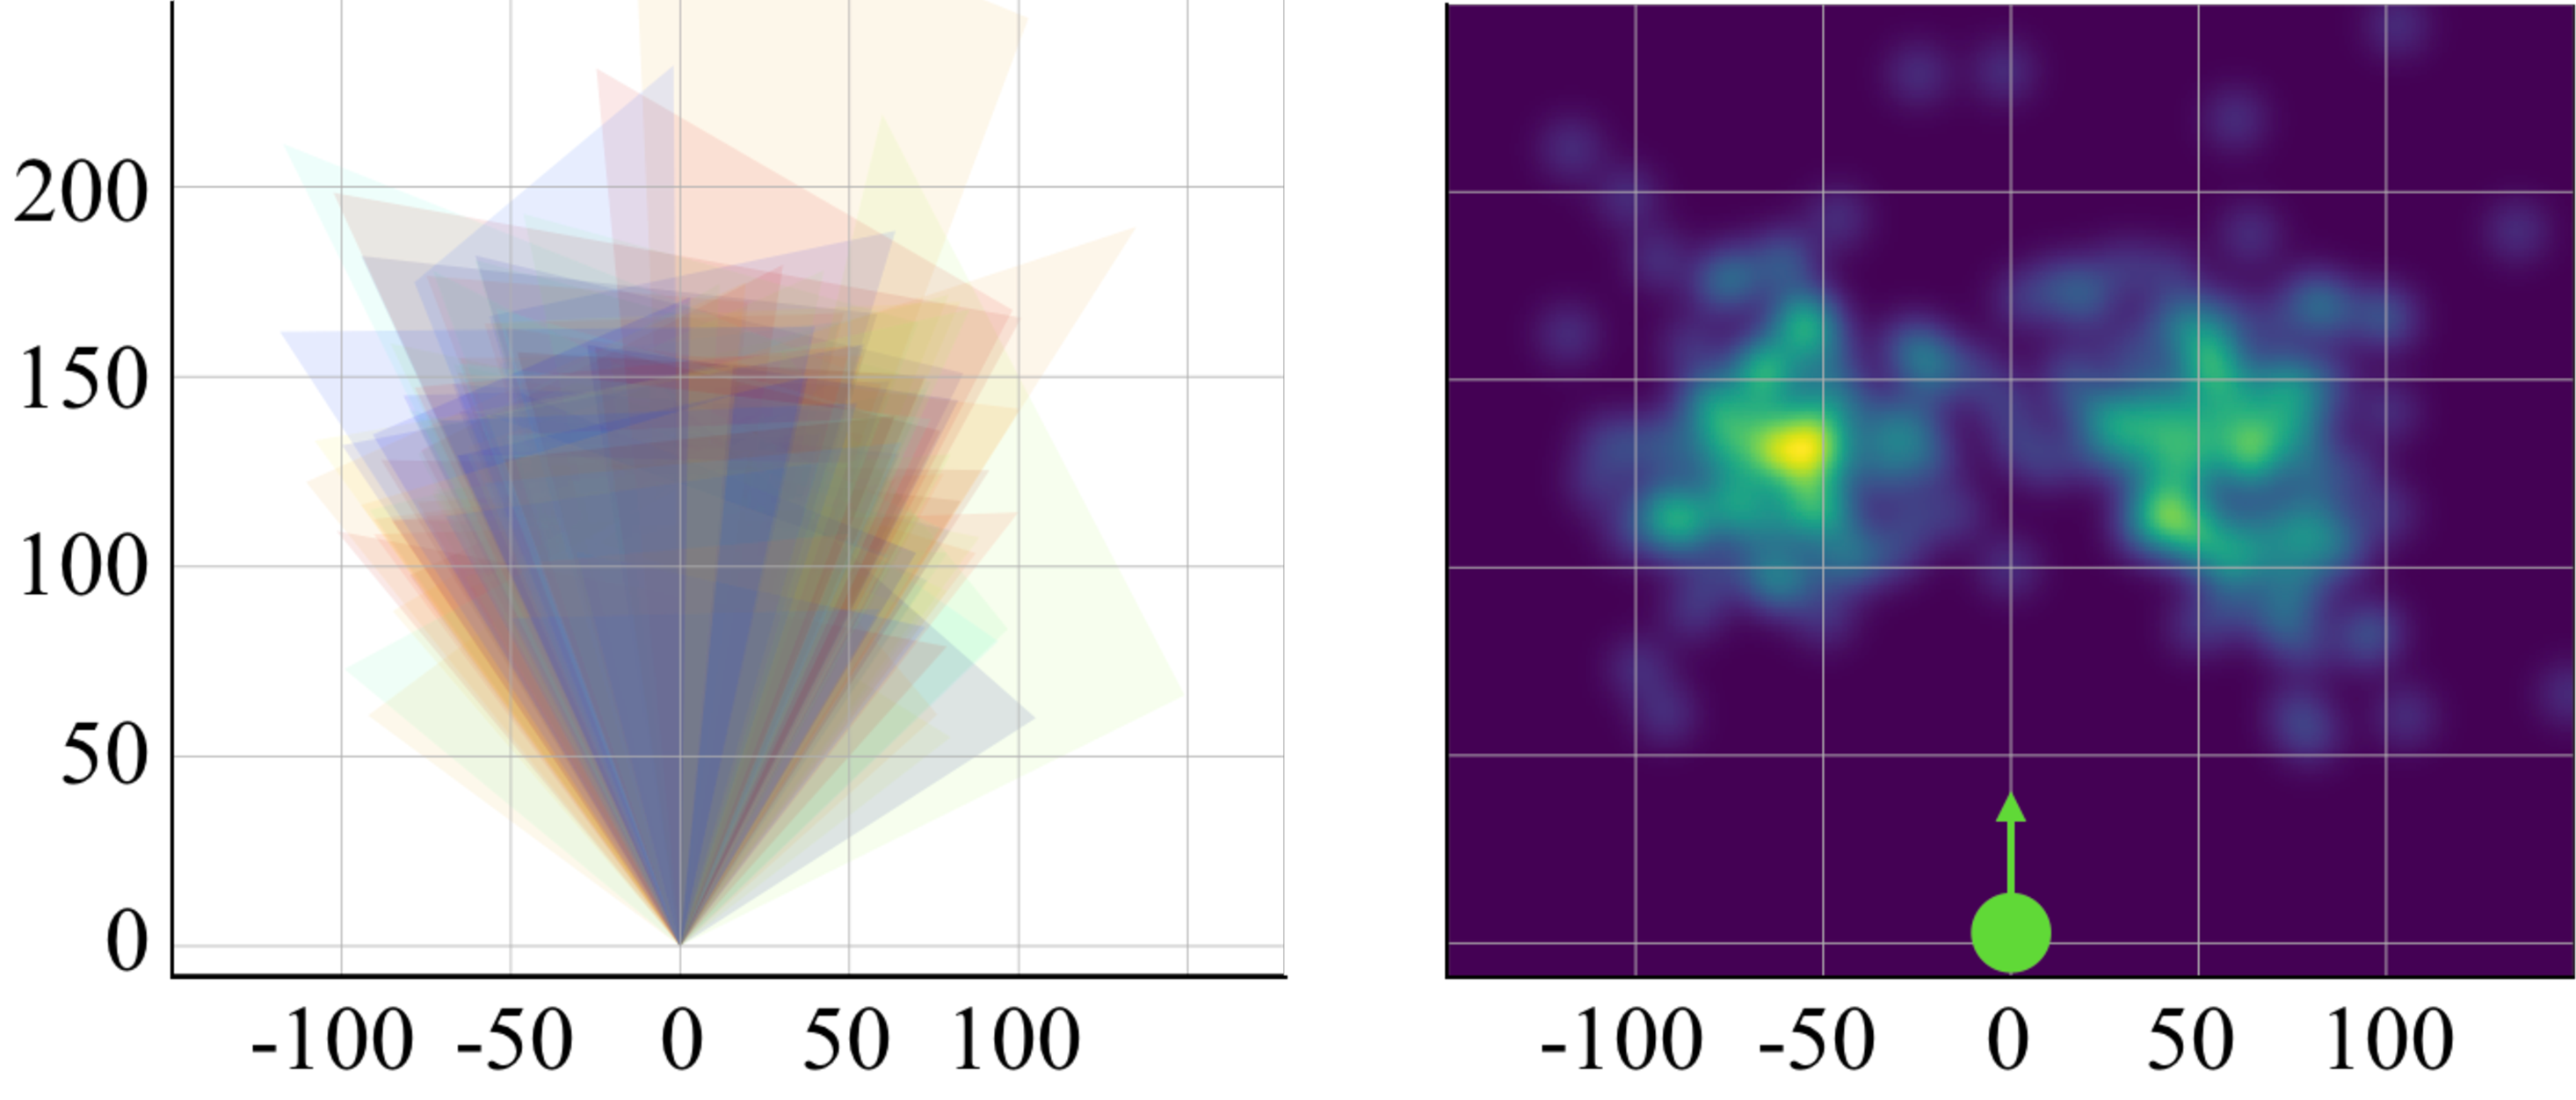
\includegraphics[ width=0.8\linewidth]{ssp_fig/haggling_proxemics_stat.pdf}
	% 	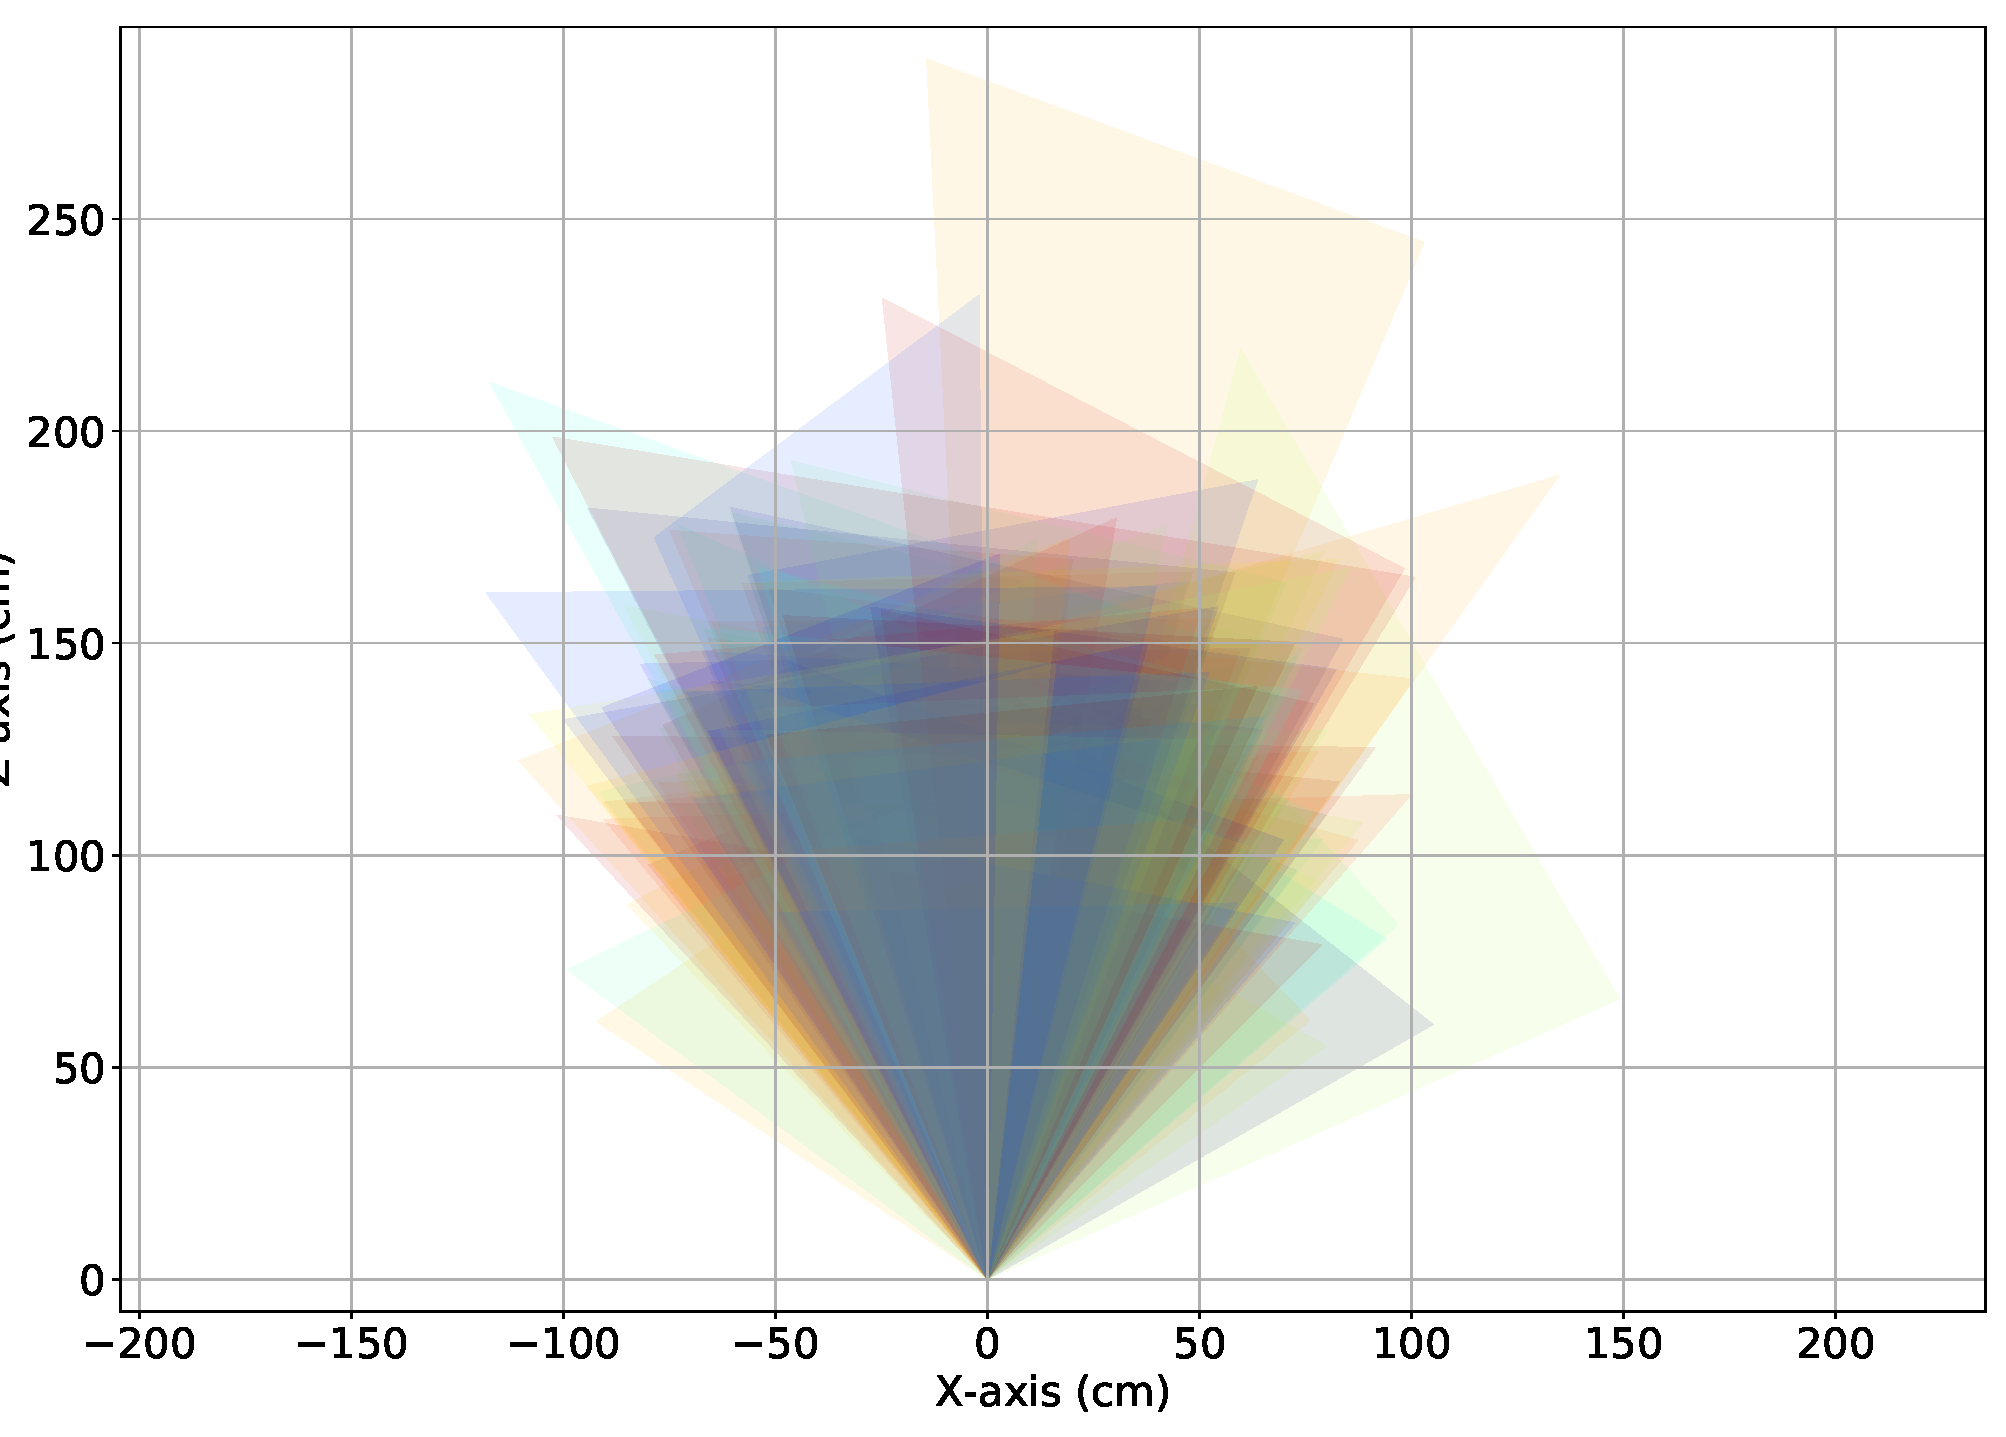
\includegraphics[trim=120 0 120 0,clip, width=0.45\linewidth]{plot/haggling_proxemics_polygon.pdf}
	% 	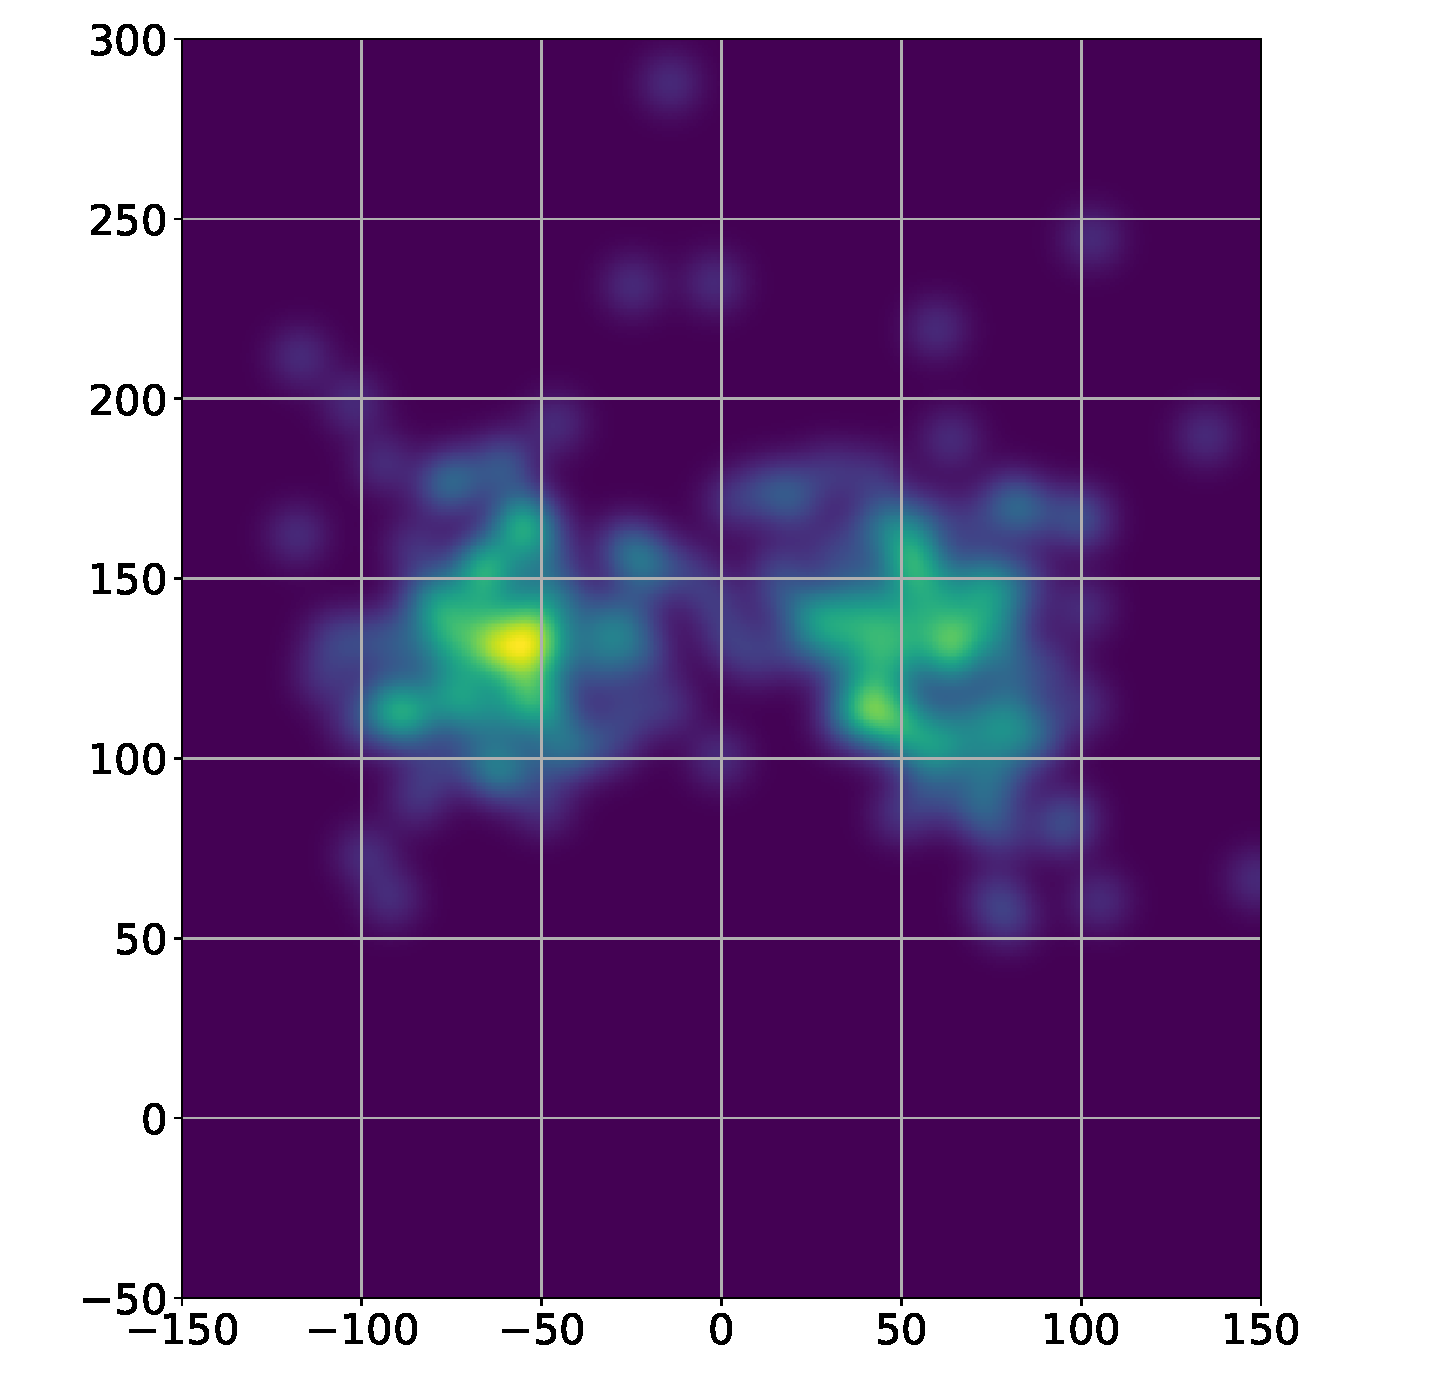
\includegraphics[width=0.45\linewidth]{plot/haggling_proxemics_heatmap.pdf} 
	%	\subfigure[TrajCompares]{\label{Fig:asso_traj}\includegraphics[width=0.5\textwidth]{img/trajCompare}}   
	\caption{Visualizing social formations in the haggling sequences as triangles (left) and a heat map (right). The formation is normalized w.r.t the buyer's location, and the green circle on the right shows the buyer location (origin) and orientation ($z$-axis).} 
	\label{fig:socialgeo_distribution}
\end{figure}

% \begin{figure}
% 	\centering       
% 	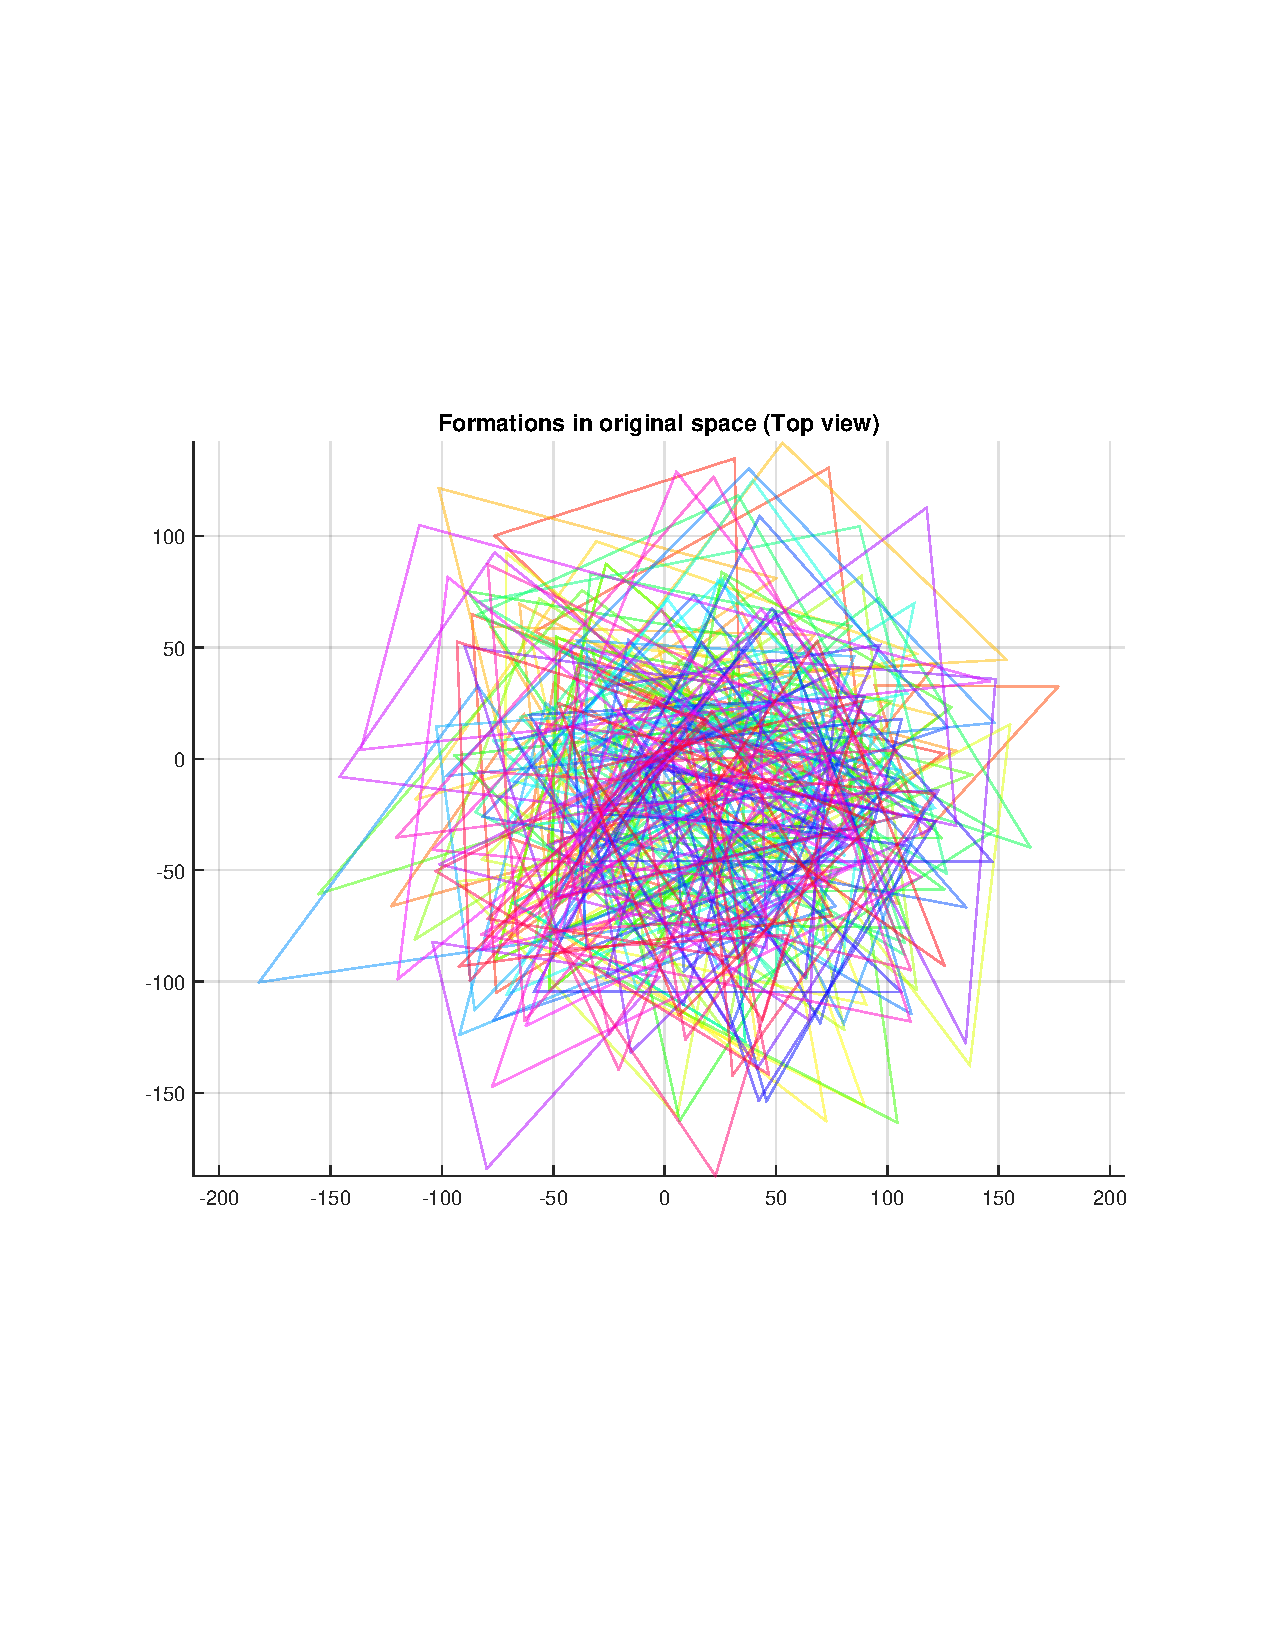
\includegraphics[trim=60 200 60 150,clip,width=0.32\linewidth]{fig/originalTri}
% 	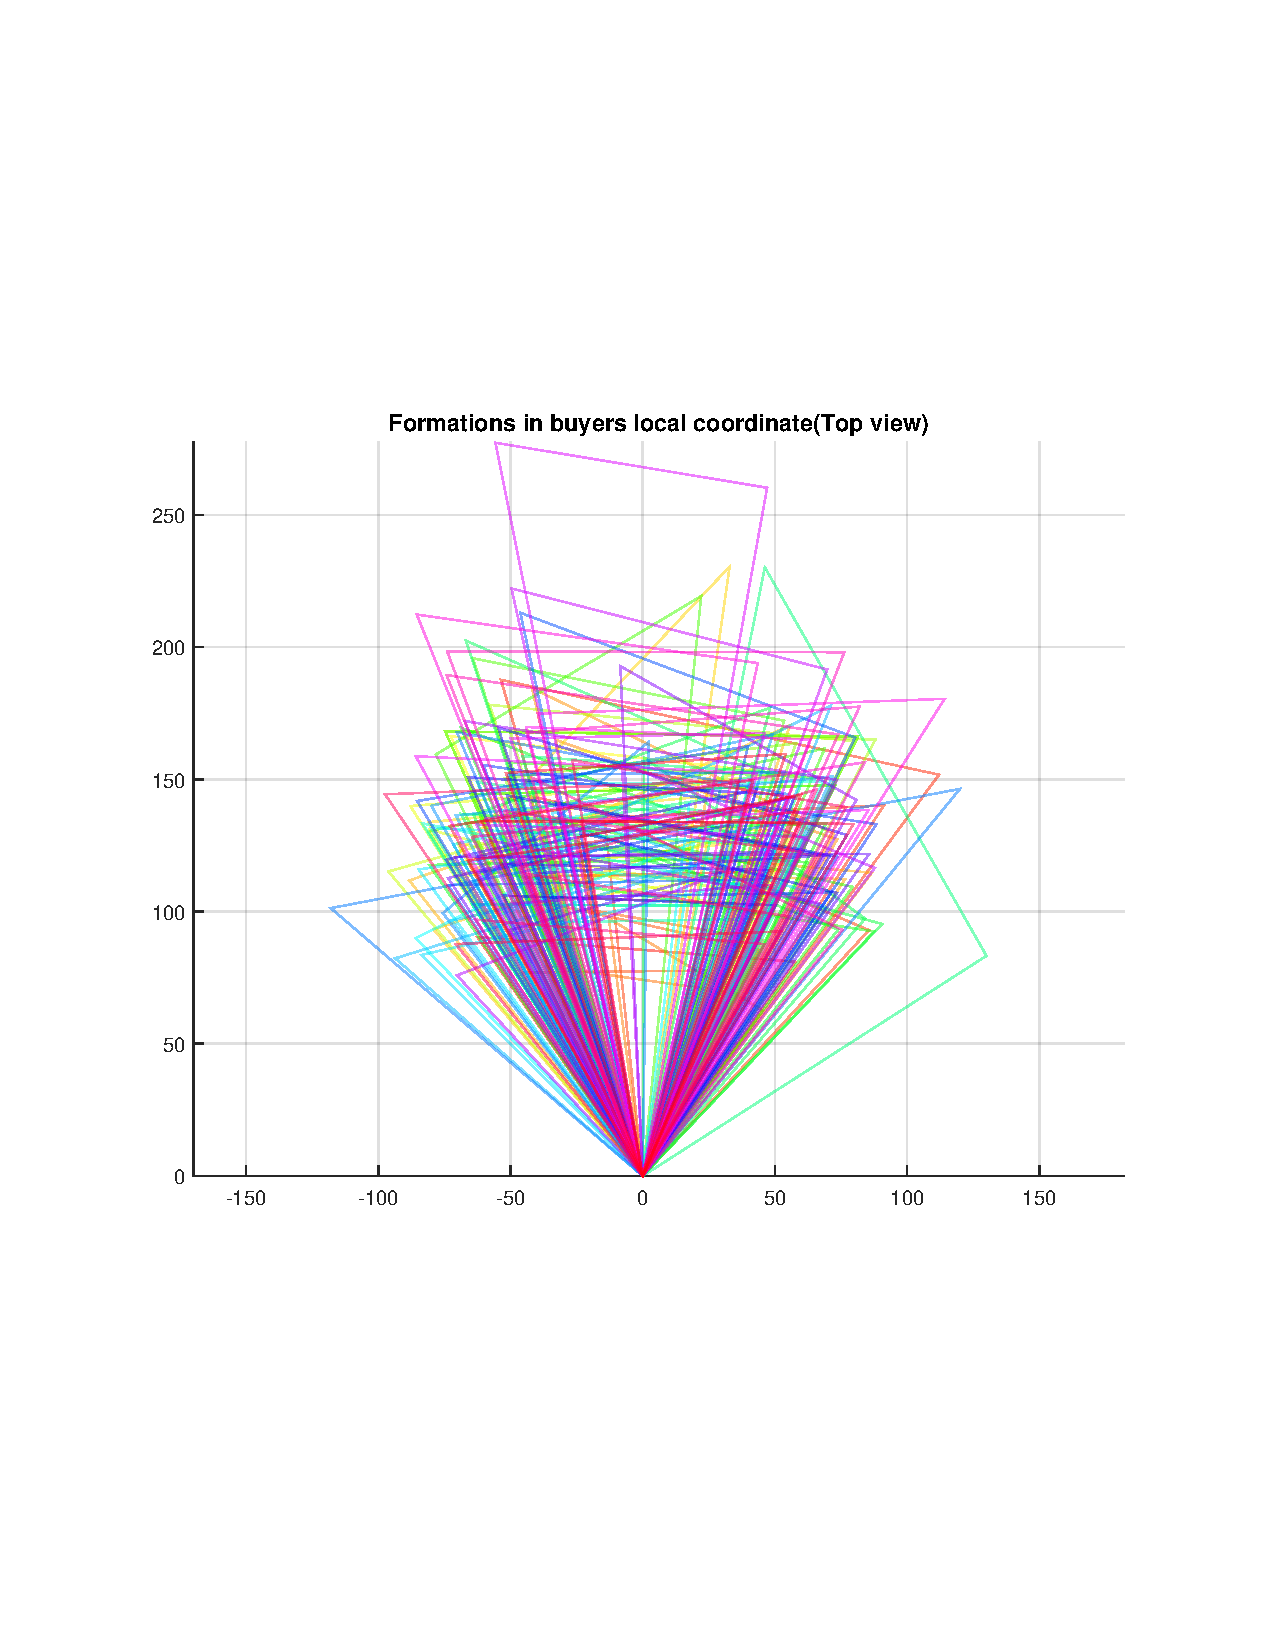
\includegraphics[trim=60 200 60 150,clip,width=0.32\linewidth]{fig/buyersTri} 
% 	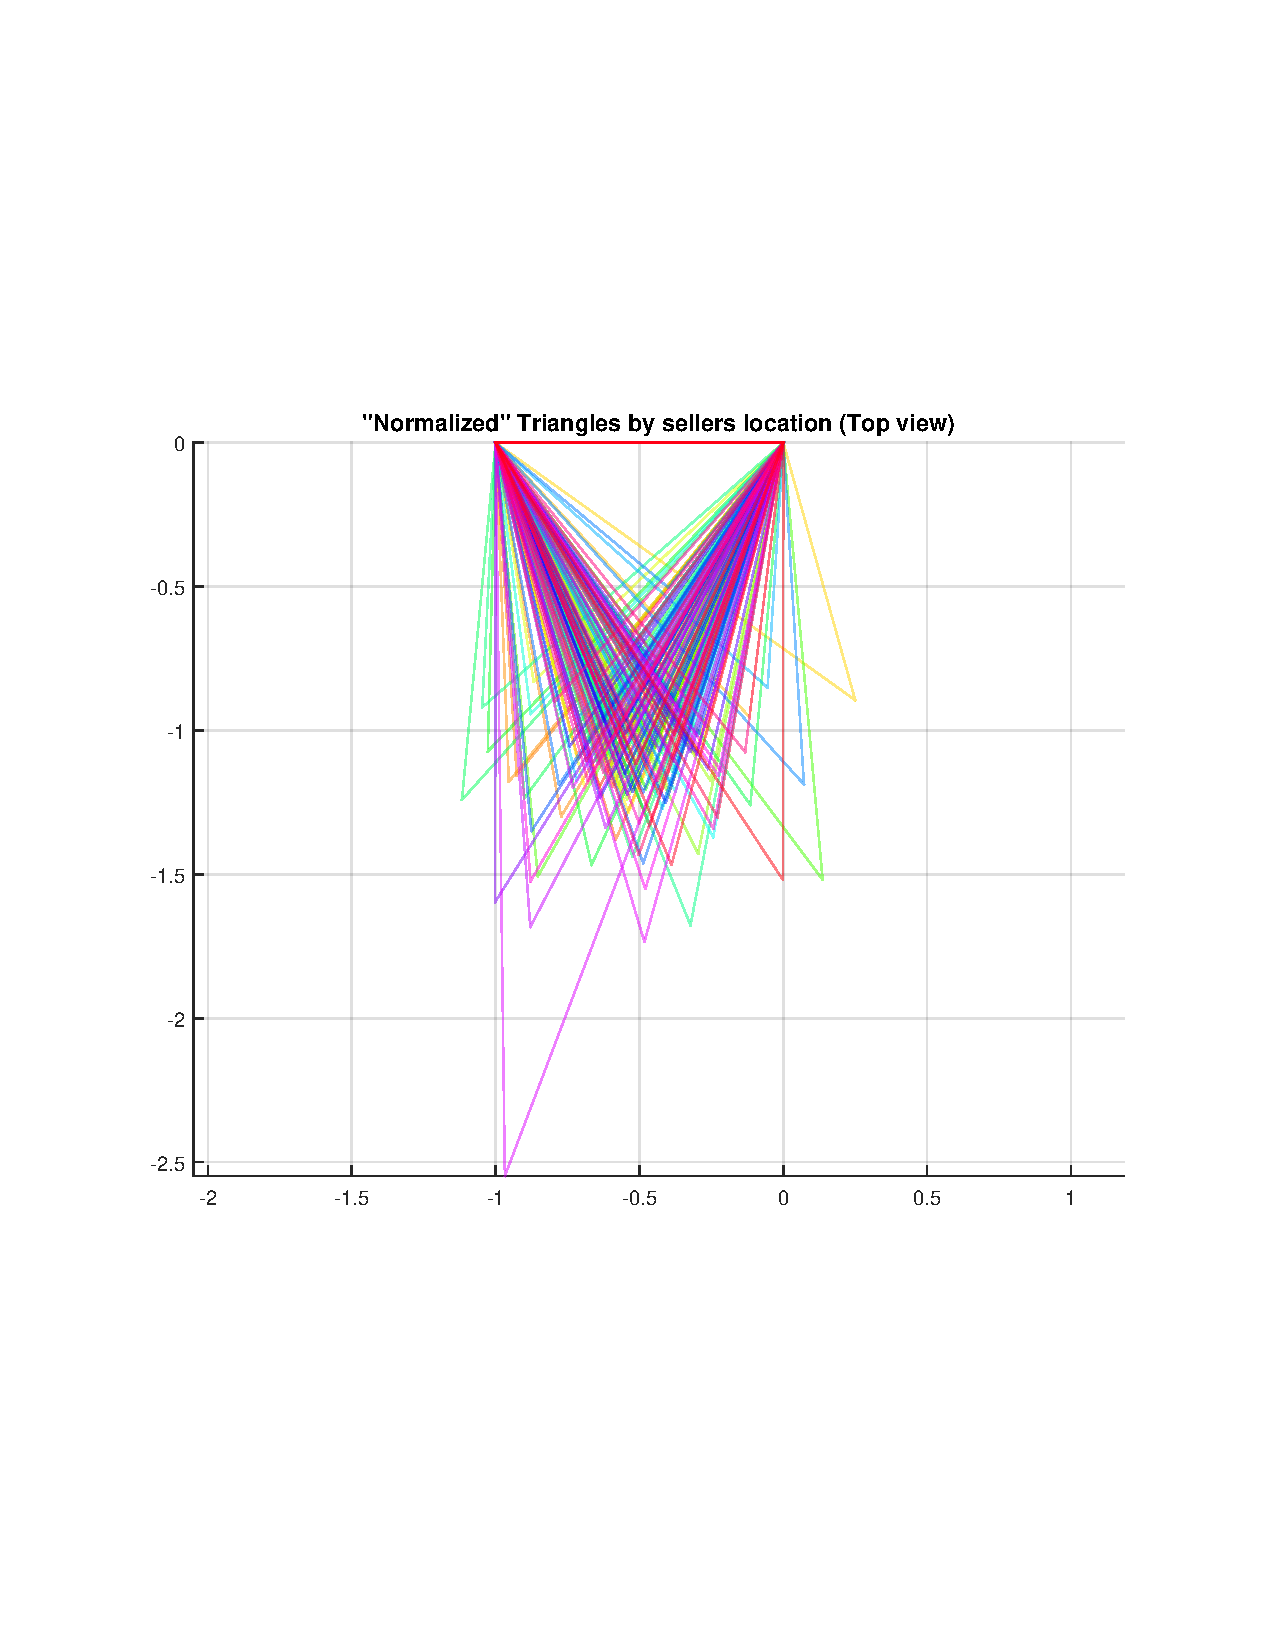
\includegraphics[trim=60 200 60 150,clip,width=0.32\linewidth]{fig/normTri} 
% 	%	\subfigure[TrajCompares]{\label{Fig:asso_traj}\includegraphics[width=0.5\textwidth]{img/trajCompare}}   
% 	\caption{Social formations in three different representations. (a) Global coordinate; (2) Person-centric coordinate defined by buyers; (3) Normalized-by-a-pair coordinate system define by two sellers} 
% 	\label{fig:socialgeo_distribution}
% \end{figure}

\subsection{Speaking Status Prediction}
We predict whether the target person is currently speaking or not by observing various other social signals in the scene. First, we consider the target individual's own social signals as input. Three different types, facial expressions, body gestures, and both of them, are used to train neural network models separately. We use the same neural network architecture for these models to fairly compare the performance, and mask out if some input signals are used. More specifically, we use the``body2speak" model in \ref{section:body2speak}, by modifying the input dimension into the concatenation of face and body signals (with $5+73$ dimensions). For body only test, we mask out the face signal part in the input with their average values, and do the similar thing if we test the model with face signal only.  The prediction accuracies from these own signals of the target person are shown in the first column of Table ~\ref{table:speaking_class}. Facial cues show the strongest correlation with speaking status, presumably due to lip motion. Own body motion also shows a strong correlation. When we use both face and body, it seems like the face signal dominates, showing a similar performance with face only case. 

More interesting experiments is performed by using the other seller's social signals as input to predict the target person's speaking status. Similar three types of social signals are considered. The result clearly shows that there exists a strong link between interpersonal social signals. The other seller's facial motion is a strong predictive cue, which presumably learns the turn-taking property in social communication.% predicting that the target person is speaking if little motion is observed from the other sellers. Other seller's body signals are also very predictive in this task. 

For the sake of comparison, we also test with the social signals of a random person, where the person is randomly selected in the testing set. As expected, the classification performance using a random person's motion as input shows about the chance level (50\%). 

%We compare the binary speaking classification performance . The task is to classify the speaking status of the target person, and we use three different body motion sources: (1) the target person's own body motion, (2) the other seller's body motion, (3) a random person's body motion. As shown in the results, the own body motion has the strongest correlation, but the other seller's body motion is also very predictive, showing that there exists a clear social link during their interaction. As expected, the classification performance using a random person's motion as input shows about the chance level (50\%). For the experiment (3), we use the same network trained for (2), but use the body motion from a subject in some other arbitrary sequence (excluding our current target sequence) as input. Presumably, the classification method using the other person's body signals learns the ``turn-taking" property in the social interaction, and predicts that the target person is speaking if little motion is observed from the other sellers (who would be listening). %This kind of study is important to make machines better understand human social behaviors, and can be facilitated from the data where natural social interactions are captured.  %This kin %shows an interesting insight that the body motions % the strong correlation of social signals can be used as a prior for predicting human behaviors. 
%\begin{table}[t]
%	\centering
%%	\footnotesize
%	\begin{tabular}{l| l| l| l}
%		\hline
%		%Types & Avg. dist. (cm) & Std.(cm) & Min dist. (cm)  & Max dist. (cm)\\
%		Input Signal & Own body & Other seller & Random person\\
%		\hline
%		%Accuracy & 80.34\% & 73.44\% & 53.39\%\\
%		%Accuracy & 76.16\% & 70.33\% & 51.05\%\\       %submitted
%		Accuracy & 80.70\% & 75.30\% & 51.05\%\\       %new
%		\hline
%	\end{tabular}
%	\caption{Speaking Classification Accuracy using different source of body motion signals as input\label{table:speaking_class}}
%\end{table}


\begin{table}[t]
	\centering
%	\footnotesize
	\begin{tabular}{c| c| c| c}
		\hline
		%Types & Avg. dist. (cm) & Std.(cm) & Min dist. (cm)  & Max dist. (cm)\\
		Input Signal Types/Sources & Self signal & Other seller's signal & Random person's signal\\
		\hline
		%Accuracy & 80.34\% & 73.44\% & 53.39\%\\
		%Accuracy & 76.16\% & 70.33\% & 51.05\%\\       %submitted
		Face+Body & 89.13\% & 77.97\% & 49.65\%\\       %new
				\hline
		Face & \underline {\textbf{89.16}}\% & \underline {\textbf{80.21}}\% & 49.64\%\\       %new
				\hline
		Body & 76.69\% & 71.29\% & 50.22\%\\       %new
		\hline
	\end{tabular}
	\caption{Speaking Classification Accuracy using different source of signals as input\label{table:speaking_class}}
\end{table}

\begin{table}[t]
	\centering
	%	\small
	%\caption{Social Formation Prediction Errors (cm) }
	\begin{tabular}{c| c| c| c}
		\hline
		%Types & Avg. dist. (cm) & Std.(cm) & Min dist. (cm)  & Max dist. (cm)\\
		Types & Position & Body Orientation & Face Orientation\\
		\hline
		PosOnly & 29.83 (13.38) & 0.26 (0.12) & 0.33 (0.13) \\
		\hline
		Pos+face & 25.23 (9.74) & 0.23 (0.09) & 0.30 (0.12) \\
		\hline
		Pos+body & 26.57 (10.24) & 0.22 (0.08) & 0.30 (0.10) \\
		\hline
		Pose+face+body & \underline {\textbf{24.59}} (10.23) &  \underline {\textbf{0.21}} (0.06) &  \underline {\textbf{0.29}} (0.09) \\
		\hline
		\hline
		Mirroring (baseline) &  50.03 (20.84) & 0.40 (0.17) & 0.52 (0.14) \\
	\end{tabular}
	\caption{Social Formation Prediction Errors (cm). Average position error between our estimation and ground-truth are reported in centimeters. The body orientation and face orientation are computed between the distance of estimated facial/body normal direction and GTs.\label{table:predForm_errors}}
\end{table}

\subsection{Social Formation Prediction (Position and Orientation)}
We predict the position and orientations of the target person, the ``left seller", by using the signals of communication partners. In this test, we explore the prediction accuracy by considering difference sources using body position, body orientation, and face orientations. Table~\ref{table:predForm_errors} shows the results. By using the all signals, we obtain the best performance. Intuitively, we can imagine that the target person's location can be estimated by triangulating the face normal direction of the other two subjects, which presumably learnt from our network. The prediction performance using only position cues shows the worst performance among them. 

For the sake of comparison, we also introduce a baseline. The baseline method (denoted as ``Mirroring" in Table~\ref{table:predForm_errors}) predicts the location of the target seller to mirror that of the other seller w.r.t the buyer's body orientation, and estimate body orientation as the average between the two input subjects. The face orientation is chosen to always face the buyer. This baseline has large errors, with poor prediction results when the buyer is directly facing the other sellers. 

%Our method shows a 25 cm error in the prediction, which is better than a baseline. As the baseline, we predict the location of the target seller to mirror that of the other seller w.r.t the buyer's body orientation, and estimate body orientation as the average between the two input subjects. The face orientation is chosen to always face the buyer (denoted as ``Mirroring" in Table~\ref{table:predForm_errors}). We also perform an ablation study to see what information is important to get better accuracy. To do this, we change the channel of the input, as in Table~\ref{table:predForm_errors}. We use the same network  but set unused input channels to their mean values in the training set. This experiment demonstrates that social formation estimation can take advantages from the body and face orientation signals. Intuitively, we can imagine that the target person's location can be estimated by triangulating the face normal direction of the other two subjects. To compute errors of orientations, we compute the 2D distance between the unit vectors representing the orientation estimation and the ground truth normal directions of face or body.% In Fig.~\ref{fig:predForm_errors}, the average position errors of each sequences are shown. 

%\begin{figure}
%	\centering
%	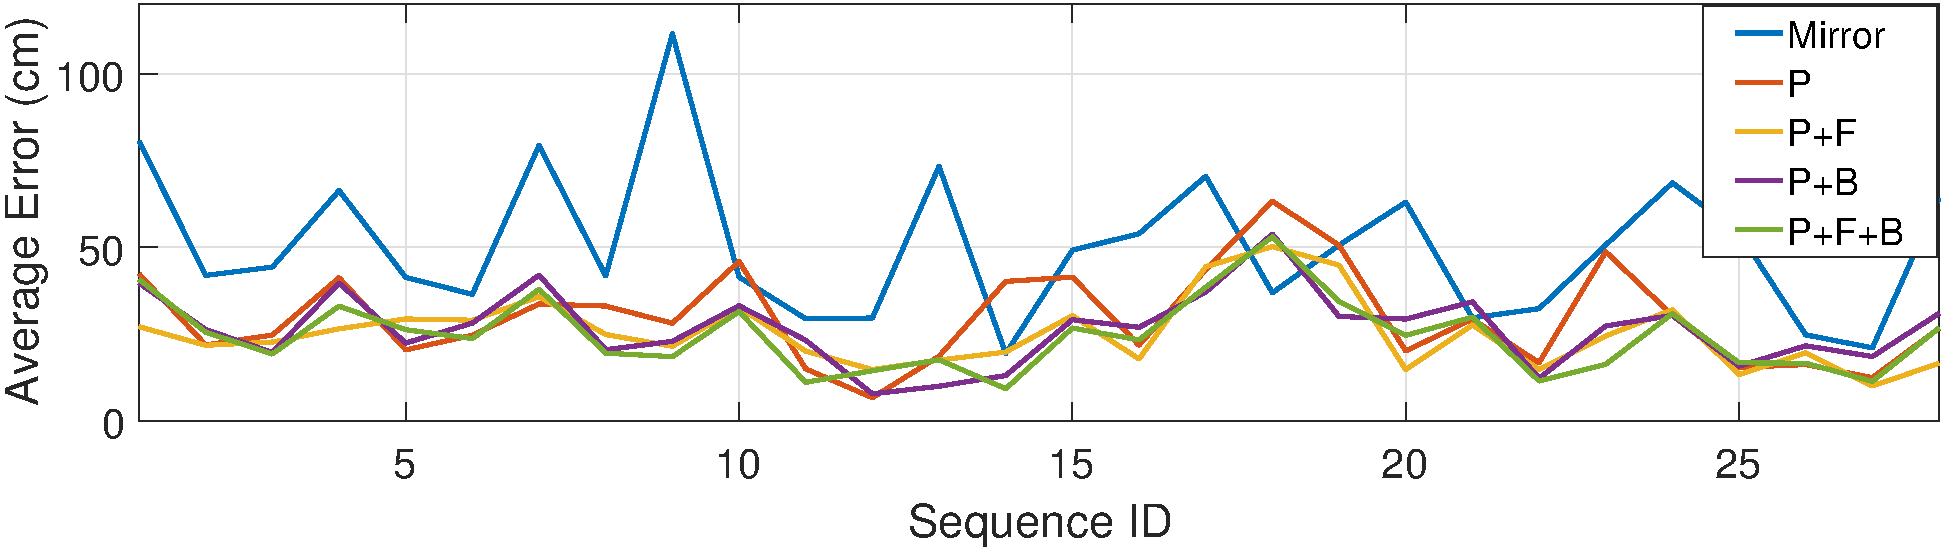
\includegraphics[width=\linewidth]{ssp_fig/cvpr19_predForm}\\
%	\includegraphics[width=\linewidth]{ssp_fig/cvpr19_predBody}
%	\caption{Average error of social formation prediction (top) and body gesture prediction (bottom). $y$-axis for the position errors in centimeters, and $x$-axis is sequence IDs.} %``Mirror" represents the baseline method, and P, F, and B denote Position, Face orientation, and Body orientation, as the input for the prediction.} 
%	\label{fig:predForm_errors}
%\end{figure}



% %Body only
% total_avg_posErr: 29.8286890398, std 13.3812589645
% total_avg_bodyOriErr: 0.263378293988, std 0.124290071428
% total_avg_faceOriErr: 0.327747834313, std 0.129691809416

% %Body + face
% total_avg_posErr: 25.2330815723, std 9.74251270294
% total_avg_bodyOriErr: 0.228412316901, std 0.0890485420823
% total_avg_faceOriErr: 0.303724261948, std 0.116639345884

% %Body + bodyOri
% total_avg_posErr: 26.57, std 10.24
% total_avg_bodyOriErr: 0.22, std 0.08
% total_avg_faceOriErr: 0.30, std 0.10

%While lower error may mean a better result, we may still see whether the prediction behave as human. 
% {\color{red} What happen when the turns are changing }

% {\color{red} Failure cases?}

% Position only, and orientation. 

% W/Wo speaking

% W/Wo body signal

% PCK curves

% Baseline: Trianglular estimation
% Orientation: See always the buyer.

% \begin{figure}
% 	\centering
% 	\includegraphics[width=\linewidth]{plot/cvpr19_predBody}
% 	\caption{Average error of body prediction. $y$-axis for the errors in centimeter, and $x$-axis for the sequences.} 
% 	\label{fig:predBody_errors}
% \end{figure}

\begin{figure*}
	\centering       
	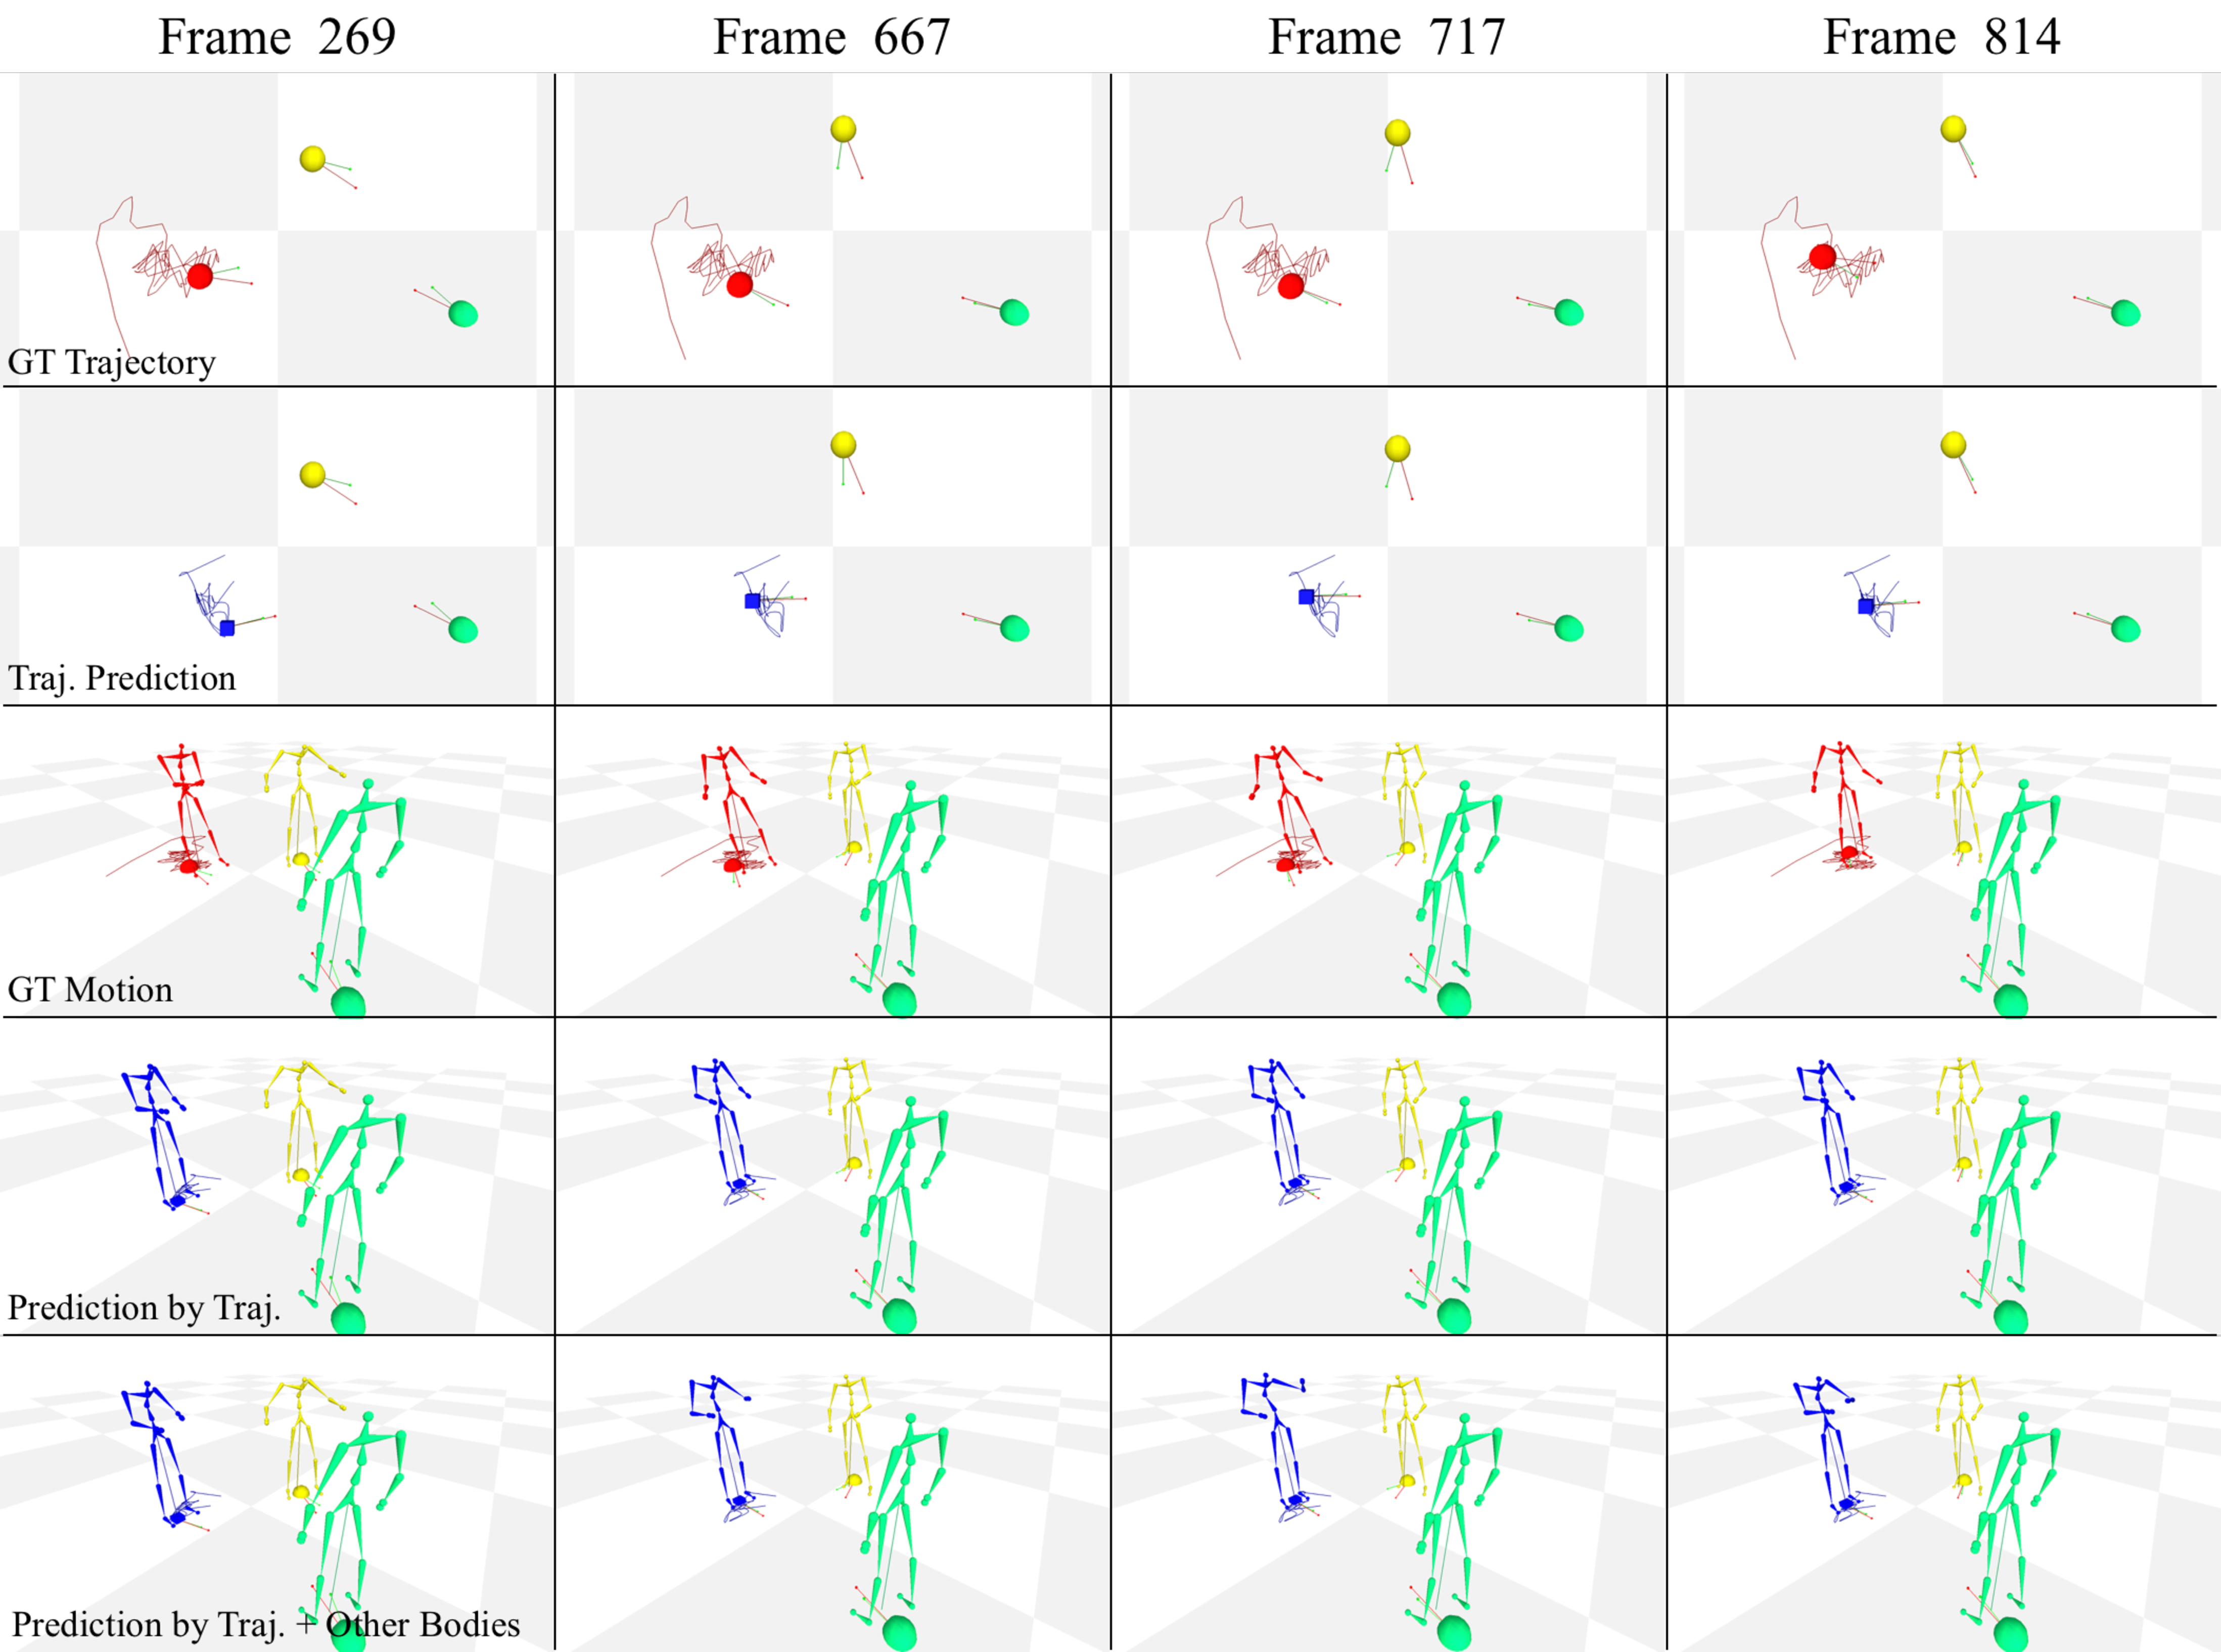
\includegraphics[width=\linewidth]{ssp_fig/qual_170221_b2_group4}
	%	\subfigure[TrajCompares]{\label{Fig:asso_traj}\includegraphics[width=0.5\textwidth]{img/trajCompare}}   
	\caption{An example result of \textit{Social Signal Prediction}. Each column shows scenes at a particular frame. The social signals drawn in green or yellow color are used as the inputs to our method, and blue signals are our social signal prediction results. The signals drawn in red are the ground truth. (First row) The ground truth social formations are shown from a top view, where the target person is shown as red spheres along with trajectories (red curves), face orientation (green arrows pointing from the spheres), and body orientations (red arrows from the spheres). (Second Row) The predicted locations (blue cubes), trajectories (blue curves), face orientations (green arrows), and body orientations (red arrows) are shown. (Third row) The ground-truth 3D body poses of the target person are shown. (Fourth row) We predict the 3D motion from the estimated 2D trajectory of the target person. (Fifth row) We use the body motion of other subjects to predict the upper body motion of the target person, which are combined to the leg body motions estimated from the trajectories.} 
	\label{fig:qualitative}
\end{figure*}

\begin{table}[t]
	\centering
%	\footnotesize
	%\caption{Social Body Gesture Prediction Errors}
	\begin{tabular}{c| c| c}
		
		\hline
		%Types & Avg. dist. (cm) & Std.(cm) & Min dist. (cm)  & Max dist. (cm)\\
		Types & Avg. Joint Errors (cm) & Std.\\
		\hline
		%Mirroring buyer & 11.60 &2.70\\
		%\hline
%		Mirroring input seller & 10.86 &2.49\\
%		\hline
		Mean Pose \underline {\textbf{7.83}} & 2.33\\
		\hline
		Traj2Body & 8.31 & 2.26\\
		\hline
		% 		body2Body & 8.19 (2.01)\\
		Body2Body & 8.72 & 2.00\\
		\hline
		% 		body2Body & 8.19 (2.01)\\
		Traj2Body (lower body) + Body2Body (upper body) & 8.61  & 1.84\\
		\hline
	\end{tabular}
	\caption{Social Body Gesture Prediction Errors (cm). Body orientation and face orientation are computed between estimated and GT unit vectors (need to be fixed) \label{table:predBody_errors}}
\end{table}



\begin{table}[t]
	\centering
	%	\footnotesize
	\begin{tabular}{l| l}
		\hline
		%Types & Avg. dist. (cm) & Std.(cm) & Min dist. (cm)  & Max dist. (cm)\\
		Input Signal & Accuracy\\
		\hline
		\hline
		Ground-truth Own Body & 79.94 \% \\       %new
				\hline
		Ground-truth Other Seller's Body & 75.28 \% \\       %new
		\hline
		\hline
		Mean Pose & 51.03\% \\       %new
				\hline
		Traj2Body & 51.42\% \\       %new
				\hline
		Body2Body & 52.97\% \\       %new
				\hline
		Body2Body+Traj2Body & 52.78\% \\       %new
				\hline
		Face2Body & \underline {\textbf{67.68}}\% \\       %new
				\hline
		Face2Body+Traj2Body & 66.60\% \\       %new
		\hline
	\end{tabular}
	\caption{We evaluate the speaking status of predicted models to quantitatively measure the quality of them. This table shows speaking status prediction accuracies, where the speaking status is predicted from the synthesized body motions from the specified sources.}
\end{table}



\subsection{Body Gestures Prediction}

We predict body motion of the target person by three methods: traj2body, body2body, and face2body. In the ``traj2body" method, the body motion is directly regressed from the estimated social formation (location and orientation) of the target person. This method shows leg motions following the trajectory movements, but has minimum upper body motion. Examples are shown in the fourth row of Fig.~\ref{fig:qualitative}. In ``body2body" method, we predict the target person's body motion by using other subjects' body motion as input. This motion does not take into account the global formation cues, but shows more dynamic body motions by responding to other subjects' motion. We can combine both methods, by merging the formation and leg motion from the first method to the upper body motion from the second method. Examples are shown in the fifth row of Fig.~\ref{fig:qualitative}. In the ``face2body" method, we use other seller's face motion as a source to predict the body motion of the target person. Similarly, we can combine this output with the leg motion of ``traj2body" method. The final prediction results show human-like social behaviors including location, body and face orientation, leg motion, and hand gestures. 

We evaluate the prediction performance of body gesture using the common L2 distance and our proposed speaking status based metric. We consider a baseline method, ``Mean Pose", by computing the average posture of all training data and constantly use it as prediction output. As shown in Table~\ref{table:predBody_errors}, the L2 error of this baseline shows the best performance, although this motion is not realistic and not suitable for the social scene.

In our new metric, we first predict the speaking status from the synthesized motion. We use the pre-trained classifier that takes own body signals as input. And then compute the accuracy by comparing the current speaking status with ground truth. This metric mainly checks the turn-taking property, penalizing the output if the synthetic motion does not follow this social rules. As described in section~\ref{section:evaluation}, the mean pose shows almost a chance level accuracy, since the motion looks not speaking at all. The prediction by ``body2body" method shows a better performance, but we found the timing of the output motion is not accurate. ``face2face" method shows the best performance, since the face cues provide a strong clue to determine the speaking timing, as demonstrated in Table~\ref{table:speaking_class}. As shown in this result, our social signal prediction method shows a reasonable performance in modeling the dynamics of social signals, and our evaluation method can be used to quantify the output.


%The final outputs predict more natural social behaviors than other baselines, satisfying most of the noticeable social rules in the scenes (distance, orientation, leg and root movement, and natural hand motions). Our results are best seen in the supplementary videos. However, the quantitative errors tend to be higher, as shown in Table~\ref{table:predBody_errors} and Figure~\ref{chapter:predBody_errors}. Notably, the average pose computed from the training set shows the best performance. This is because the error metric computing the 3D errors from the ground-truth cannot fully evaluate how natural the motion appears. %Given the similar social signal inputs, there are diverse possible suitable human motions, and a better evaluation method is required to consider this.%  the quality of social signal prediction.% and it should be related to a 

% {\color{red} Qualitative example where turn taking is captured?}

% \noindent \textbf{Direct Regression from Social Formations:}
% We can directly regress from the predicted 2D formation output.  

% PCK curves 
% Per joint


% \textbf{Regression from Richer Input:}
% We use other skeletons and input and see any improvement. 

% Compared to the direct regression. 
% {\color{red} Any semantic improvement which is not captured by numbers?}

% Any good way to evaluate realistic human motion???


% \subsection{Quantifying Social Signal Importance}



% \subsection{Correlation between Body, Face, and Hands}

% We use all body parts for communication where each part plays a role to send some specific signals. Unfortunately, these roles are also poorly understood. In this section, we investigate whether there exists patterns or strong correlations among parts. We study this by predicting a missing part given other body parts. 

% Body2face, face2body

% \subsection{Face and Hands signals}

\subsection{Discussion}
We introduce a social signal prediction task, to ultimately endow machines with the ability to socially interact with humans. For this objective, we present a large-scale social interaction dataset where the full-spectrum of multi-modal social signals are measured on a carefully designed negotiation scenario. Our dataset can play an important role to understand the correlation and causality of diverse channels of social signals by applying computational methods. Our baseline results show a potential to exploit our dataset to mimic human behaviors. As a core open question, a better evaluation metric is required to quantify natural social behaviors. Collecting social interaction dataset in-the-wild should be another important future direction to study social interactions at scale. %In our work, we mainly focus on triadic interactions, but more general social scenarios also need to be considered.

% Additional cues, face and body orientation, is helpful to better estimate the location. But the improvement is not so big. And no obvious qualitative evidence is found. I guess this is due to the limited representation way for the angles.

% Easy work can be done and easily noticeable. Hard one is hard since is is less noticeble. What is the missing piece?

% \section{Using social cues to predict other people's signal}
% The use of social cues are important to guess the target person's signal, assuming body signals are used for sicial interaction. For example, if we know that a person is speaking, this can be a cue that other people are listening (e.g., high probabity of nodding). In this section, we see that other people's cues (social geometry, face, body, speaking) can be helpful to predict target subject's social signal



% \subsection{Social Formation 2 Body}

% Trajectory and orientation prediction --- Body motion inference (legs)

% Speaking signal --- Body motion inference



% \section{Higher level social signal understanding}


% \subsection{Winner Classifcation: What makes motion more persuasive?)}


% \subsection{Quantitying Social Signal: What part is more influential}
% Attention model? Just simple weighting?
% LInear model to get some scalar value for each feature... Softmax (to make sum as one) ... weighting....

% \subsection{Real vs Fake social interaction?}



%
%
%\subsection{By Using Body and Face Orientation}
%
%
%Input: Two people location + orientation of face
%output: location and orientation of the target person
%
% 
%Baseline: given two people, regress another person. 
%Absolute location with embedding?
%Relative location
%
%Comparison to Hall's model. F-formation
%
%GAN loss: add gan loss
%
%
%
%\section{Body based Speaking/Silence Classification}
%
%\section{Face based Speaking/Silence Classification}
%
%
%\section{Speaking Signal to Face generation}
%
%
%\section{Speaking Signal to Other people's Speaking Signal Generation}
%
%
%\section{Speaking Signal}



%
%
%{\small
%\bibliographystyle{ieee}
%\bibliography{socialSignal,thesis}
%}

